%Set the document class and font size
\documentclass[fleqn, bachelor,subf,12pt,notitlepage]{article}
\usepackage[utf8]{inputenc}
\usepackage{enumerate}
\usepackage{amsmath}
\usepackage{mathtools} 
\usepackage{amssymb}
\usepackage{systeme}
\usepackage[english]{babel}
\usepackage{xparse}
\usepackage{xfrac}
\usepackage{setspace}
\usepackage{multicol}
\usepackage{array}
\usepackage{tabularx}
\usepackage{bigints}
\usepackage{fontspec}
\usepackage{chngcntr}
\usepackage{caption}

%This package allows to change figure insertion mode (H, etc.)
\usepackage{float}

%This package is used for big sum symbol
\usepackage{relsize}


%This command puts section number after section name
%\usepackage[explicit]{titlesec}
%\titleformat{\section}{\normalfont\Large\bfseries}{}{0em}{#1\ \thesection}

%This command allows to add section number in figure caption
%\counterwithin{figure}{section}

%This command help to keep counting but allows not to print the number of the section, etc.
%\renewcommand\thesection{}
%\renewcommand\thesubsection{}

%Change command to armenian
%\addto\captionsenglish{\renewcommand{\figurename}{Նկար}}

%This is a command for creating new command for reducing the size of the given math equation
\newcommand\scalemath[2]{\scalebox{#1}{\mbox{\ensuremath{\displaystyle #2}}}}

\usepackage
[
 	a4paper,
 	left=30mm,
	right = 10mm,
 	top=20mm,
	bottom=25mm
 ]
{geometry}

%This command sets the font
\setmainfont{GHEA Grapalat}

%These commands change line spacing
%\onehalfspacing
\linespread{1.5}

\title{Դիպլոմային աշխատանք}
\author{Կամո Սևոյան}

%This command allows to change page counter.
\setcounter{page}{4}

\begin{document}

%This command allows to correctly
\sloppy

%This command builds content automatically
%	\tableofcontents

\section*{\centering Գլուխ 1\\ Միաչափ ինտերպոլյացիա}
\subsection*{1.1 Էրմիթյան ինտերպոլյացիա}
\hspace{\parindent}Նախքան անդրադառնալը բազմաչամ ինտերպոլյացիայի խնդրին, քննարկենք մեկ փոփոխականի ֆունկցիայի ինտերպոլյացիայի որոշ դետալներ։

Ենթադրենք տրված են $f:\Omega \mapsto \Theta, \Omega, \Theta \subset \mathbb{R}$ ֆունկցիան,  $\left\{x_{i}\right\}_{i=0}^{N}$ կետերը և դրանց համապատասխան $\left\{y_{i}=f\left(x_{i}\right)\right\}_{i=0}^{N}$ արժեքները։ Յուրաքանչյուր $\left[x_{i}, x_{i+1}\right]$ հատվածում  ինտերպոլացնող ֆունկցիան իրենից ներկայացնում է գխային ֆունկցիա, որը կարելի է ներկայացնել հետևյալ տեսքով.
\begin{equation}
p_{1}^{(i)}\left(x\right)=\dfrac{x_{i+1}-x}{x_{i+1}-x_{i}}y_{i}+\dfrac{x-x_{i+1}}{x_{i+1}-x_{i}}y_{i+1}, i=\overline{0, N-1}
\end{equation}
Այսպիսով $\left[x_{0}, x_{N}\right]$ հատվածում կտոր առ կտոր մոտարկող ֆունկցիան տրվում է հետևյալ կերպ.
\begin{equation}
p_{1}\left(x\right)=\sum_{i=0}^{N}\varphi_{i} \left(x\right)y_{i}
\end{equation}
Որտեղ 
\begin{equation}
\begin{aligned}
\varphi_{0}\left(x\right)&=\begin{cases}
\dfrac{x_{1}-x}{x_{1}-x_{0}}, x\in \left[x_{0}, x_{1}\right]\\
0, x\in \left[x_{1}, x_{N}\right]\\
\end{cases}\\
\varphi_{i}\left(x\right)&=\begin{cases}
0, x\in \left[x_{0}, x_{i-1}\right]\\
\dfrac{x-x_{i-1}}{x_{i}-x_{i-1}}, x\in \left[x_{i-1}, x_{i}\right]\\
\dfrac{x_{i+1}-x}{x_{i+1}-x_{i}}, x\in \left[x_{i}, x_{i+1}\right]\\
0, x\in \left[x_{i+1}, x_{N}\right]\\
\end{cases}\\
\varphi_{N}\left(x\right)&=\begin{cases}
0, x\in \left[x_{0}, x_{N-1}\right]\\
\dfrac{x-x_{N-1}}{x_{N}-x_{N-1}}, x\in \left[x_{N-1}, x_{N}\right]\\
\end{cases}
\end{aligned}
\end{equation}
$\varphi_{i}\left(x\right)$ ֆունկցիաները կոչվում են բազիսային ֆունկցիաներ, որոնք ունեն այսպես կոչված լոկալ կրողներ, քանի որ դրանք ոչ զրոյական են որևէ տիրույթում և զրոյական որոշման տիրույթի մնացած մասերում։
Նմանատիպ բազիսային ֆունկցիաների հիմնական հատկությունն այն է, որ դրանք հավասար են մեկի որևէ կոնկրետ հանգույցում և հավասար են զրոյի մնացած բոլոր հանգույցներում։ Նշենք սակայն, որ այս տիպի ինտերպոլյացիան $C^{0}$ դասի է, այսինք միայն անընդհատ է, և հետևաբար կիրառելի չէ այն խնդիրներում, որտեղ պահանջվում է ավելի բարձր կարգի ողորկություն։
\begin{figure}[H]
\centering
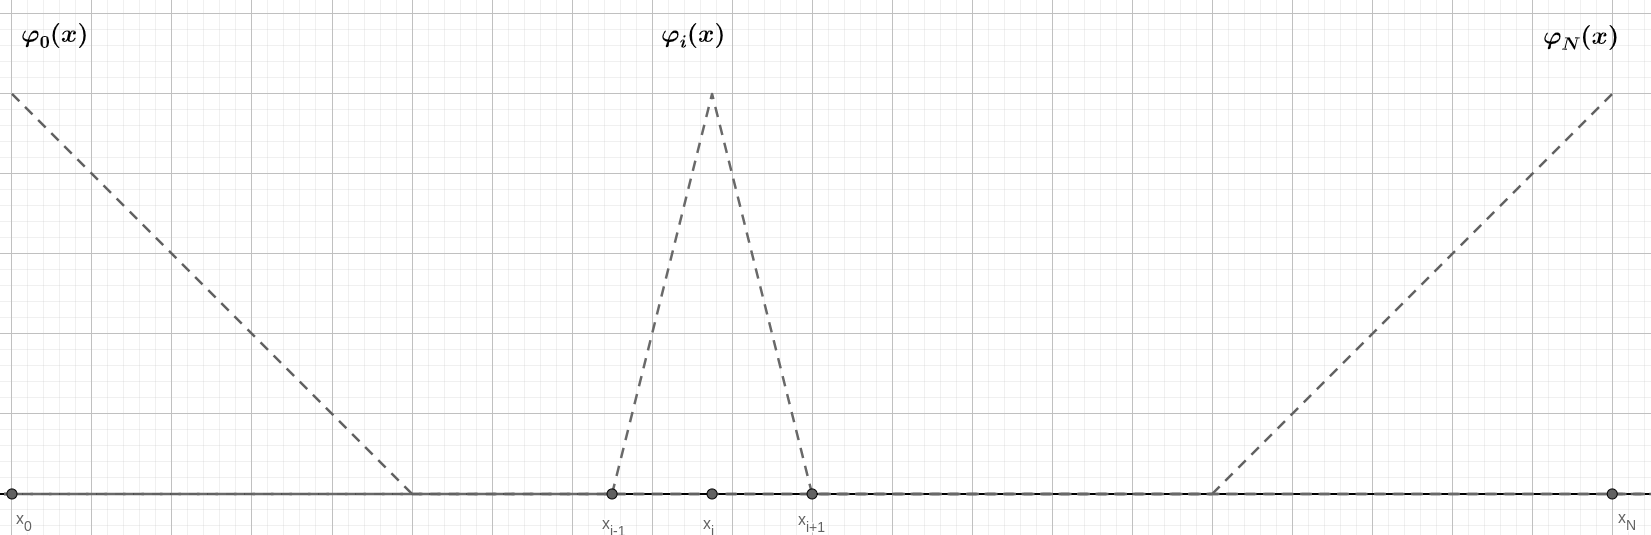
\includegraphics[width=1.0\textwidth]{images/one_var_linear}
\captionsetup{labelformat=empty}
\caption{Նկար 1.1. Գծային ինտերպոլյացիայի բազիսային ֆունկցիաներ։}
\end{figure}
Այժմ դիտարկենք հետևյալ խնդիրը. անհրաժեշտ է կառուցել  կտոր առ կտոր մոտարկող ֆունկցիա, որը ֆունկցիայի արժեքի հետ մեկտեղ կհամըկնի նաև ֆունկցիայի առաջին կարգի ածանցյալի արժեքի հետ ինտերպոլյացիոն հանգույցներում։ Այսինքն.
\begin{equation}
\dfrac{d^{j}}{dx^j}f(x_{i})=\dfrac{d^{j}}{dx^j}p_{3}(x_{i}),   \; j=0, 1;  \; i=\overline{0, N-1}
\end{equation}
Յուրաքանչյուր $\left[x_{i}, x_{i+1}\right]$ հատվածում ինտերպոլյացիոն ֆունկցիան իրենից ներկայացնում է խորանարդային ֆունկցիա, որը կարելի է ներկայացնել հետևյալ տեսքով։
\begin{equation}
p_{3}^{\left(i\right)} = \alpha_{i}(x)f(x_{i})+\beta_{i+1}(x)f(x_{i+1})+\gamma_{i}(x)f^{'}(x_{i})+\delta_{i+1}(x)f^{'}(x_{i+1})
\end{equation}
որտեղ 
\begin{equation}
\begin{aligned}
&\alpha_{i}(x)=\dfrac{\left(x_{i+1}-x\right)^{2}\left[\left(x_{i+1}-x_{i}\right)+2\left(x-x_{i}\right)\right]}{\left(x_{i+1}-x_{i}\right)^{3}}\\
&\beta_{i+1}(x)=\dfrac{\left(x-x_{i}\right)^{2}\left[\left(x_{i+1}-x_{i}\right)+2\left(x_{i+1}-x\right)\right]}{\left(x_{i+1}-x_{i}\right)^{3}}\\
&\gamma_{i}(x)=\dfrac{\left(x-x_{i}\right)\left(x_{i+1}-x\right)^{2}}{\left(x_{i+1}-x_{i}\right)^{2}}, \; \delta_{i+1}(x)=\dfrac{\left(x-x_{i}\right)^2\left(x-x_{i+1}\right)}{\left(x_{i+1}-x_{i}\right)^{2}}
\end{aligned}
\end{equation}
Այսպիսով $\left[x_{0}, x_{N}\right]$ հատվածում կտոր առ կտոր մոտարկող ֆունկցիան ներկայացվում է բազիսային ֆունկցիաների գծային կոմբինացիայի տեսքով.
\begin{equation}
p_{3}(x)=\sum_{i=0}^{N}\left[\varphi_{i}^{(0)}f(x_{i})+\varphi_{i}^{(1)}f^{'}(x_{i})\right]
\end{equation}
որտեղ 

\begin{equation}
\begin{aligned}
\varphi^{(0)}_{0}\left(x\right)&=\begin{cases}
\dfrac{\left(x_{1}-x\right)^{2}\left[\left(x_{1}-x_{0}\right)+2\left(x-x_{0}\right)\right]}{\left(x_{1}-x_{0}\right)^{3}},  x\in \left[x_{0}, x_{1}\right]\\
0, x\in \left[x_{1}, x_{N}\right]\\
\end{cases}\\
\varphi^{(0)}_{i}\left(x\right)&=\begin{cases}
0, x\in \left[x_{0}, x_{i-1}\right]\\
\dfrac{\left(x-x_{i-1}\right)^{2}\left[\left(x_{i}-x_{i-1}\right)+2\left(x_{i}-x\right)\right]}{\left(x_{i}-x_{i-1}\right)^{3}}, x\in \left[x_{i-1}, x_{i}\right]\\
\dfrac{\left(x_{i+1}-x\right)^{2}\left[\left(x_{i+1}-x_{i}\right)+2\left(x-x_{i}\right)\right]}{\left(x_{i+1}-x_{i}\right)^{3}}, x\in \left[x_{i}, x_{i+1}\right]\\
0, x\in \left[x_{i+1}, x_{N}\right]\\
\end{cases}\\
\varphi^{(0)}_{N}\left(x\right)&=\begin{cases}
0, x\in \left[x_{0}, x_{N-1}\right]\\
\dfrac{\left(x-x_{N-1}\right)^{2}\left[\left(x_{N}-x_{N-1}\right)+2\left(x_{N}-x\right)\right]}{\left(x_{N}-x_{N-1}\right)^{3}}, x\in \left[x_{N-1}, x_{N}\right]\\
\end{cases}
\end{aligned}
\end{equation}

\begin{equation}
\begin{aligned}
\varphi^{(1)}_{0}\left(x\right)&=\begin{cases}
\dfrac{\left(x-x_{0}\right)\left(x_{1}-x\right)^{2}}{\left(x_{1}-x_{0}\right)^{2}}, x\in \left[x_{0}, x_{1}\right]\\
0, x\in \left[x_{1}, x_{N}\right]\\
\end{cases}\\
\varphi^{(1)}_{i}\left(x\right)&=\begin{cases}
0, x\in \left[x_{0}, x_{i-1}\right]\\
\dfrac{\left(x-x_{i-1}\right)^2\left(x-x_{i}\right)}{\left(x_{i}-x_{i-1}\right)^{2}}, x\in \left[x_{i-1}, x_{i}\right]\\
\dfrac{\left(x-x_{i}\right)\left(x_{i+1}-x\right)^{2}}{\left(x_{i+1}-x_{i}\right)^{2}}, x\in \left[x_{i}, x_{i+1}\right]\\
0, x\in \left[x_{i+1}, x_{N}\right]\\
\end{cases}\\
\varphi^{(1)}_{N}\left(x\right)&=\begin{cases}
0, x\in \left[x_{0}, x_{N-1}\right]\\
\dfrac{\left(x-x_{N-1}\right)^{2}\left(x-x_{N}\right)}{\left(x_{N}-x_{N-1}\right)^{2}}, x\in \left[x_{N-1}, x_{N}\right]\\
\end{cases}
\end{aligned}
\end{equation}

\begin{figure}[h]
\centering
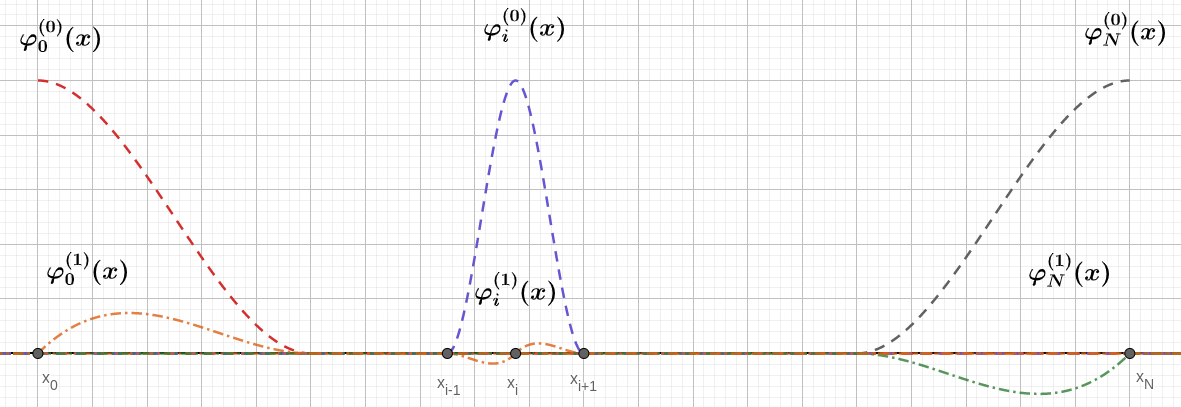
\includegraphics[width=0.9\textwidth]{images/one_var_quadratic}
\captionsetup{labelformat=empty}
\caption{Նկար 1.2. երկրորդ կարգի էրմիթյան ինտերպոլյացիայի բազիսային ֆունկցիաներ։}
\end{figure}
Վերը ներկայացված ինտերպոլյացիաների օրինակները էրմիթյան ինտերպոլյացիայի մասնովոր դեպքեր են համապատասխանաբար 1 և 2 կարգերի դեպքում։
Ընդհանուր դեպքում m֊րդ կարգի էրմիթյան ինտերպոլյացիայի պայմանը կարելի է գրել հետևյալ կերպ.
\begin{equation}
\dfrac{d^{k}}{dx^{k}}f\left(x_{i}\right)=\dfrac{d^{k}}{dx^{k}}p_{2m-1}\left(x_{i}\right), \;  i=\overline{0, N}, \;  k=\overline{0, m-1}
\end{equation}
\newpage

\subsection*{1.2 Քառակուսային և խորանարդային ինտերպոլյացիա}
Խնդիրներում, որտեղ անհրաժեշտ է որոշել միայն տրված ֆունկիցիան, ֆունկցիայի ածանցյալներն ինտերպոլացնելու փոխարեն դրվում է դրանց անընդհատության պայման հանգուցային կետերում,  բավականին հեշտացնելով դրված խնդիրը և դրա լուծումը։
Նման տիպի ինտերպոլյացիայի կառուցման պարզագույն օրինակը հետևյալն է.
Յուրաքանչյուր $\left[x_{i}, x_{i+1}\right]$ ինտերվալում կառուցվում է այպիսի պարաբոլ, որ բոլոր $x_{i}$ հանգուցային կետերում առանջին կարգի ածանցյալները լինեն անընդհատ։
\begin{equation}
S_{2}^{(i)}(x)=f(x_{i})+\dfrac{f(x_{i+1})-f(x_{i})}{x_{i+1}-x_{i}}\left(x-x_{i}\right)+c_{i}\left(x-x_{i}\right)\left(x-x_{i+1}\right)
\end{equation}
Ածանցյալների անընդհատության պայմանից կհետևի, որ
\begin{equation}
c_{i}+c_{i-1}=\dfrac{1}{h^{2}}\left(f(x_{i+1})-2f(x_{i})+f(x_{i-1})\right) \; i=\overline{1, N-1}
\end{equation}
Քանի որ համակարը պարունակում է $N-1$ հավասարում, ապա մնում է մեկ ազատ գործակից, որը կարելի գտնել, որևէ $x_{j}$ հանգուցային կետում որոշելով $S_{2}^{(j)''}$֊ն։

Առավել կիրառելի են խորանարդային սփլայնները։ Այս դեպքում յուրաքանչյուր $\left[x_{i}, x_{i+1}\right]$ ինտերվալում կառուցվում են երրորդ աստիճանի բազմանդամներ այնպես, որ հանգույցներում առաջին և երկրորդ կարգի ածանցյալները լինեն անընդհատ։ 
Բազմանդամը դիտարկելու փոխարեն դիտարկենք նրա երկրորդ կարգի ածանցյալը: Այն գծային ֆունկցիա է, հետևաբար այն կարելի է ներկայացնել հետևյալ տեսքով.
\begin{equation}
S^{(i)''}_3(x)=c_{i}\dfrac{x_{i+1}-x}{x-x_{i}}+c_{i+1}\dfrac{x-x_{i}}{x_{i+1}-x_{i}}
\end{equation}
\noindent որտեղ $c_{i}$ և $c_{i+1}$֊ը $x_{i}$ և $x_{i+1}$ կետերում երկրորդ կարգի ածանցյալների արժենքներն են։ 
\noindent Հաշվի առնելով ինտերպոլյացիոն և անընդհատության պայմանները.

\begin{equation}
\begin{cases}
				S_{3}^{(i)}(x_{i}) &=f_{i}\\
				S_{3}^{(i)}(x_{i+1}) &= f_{i+1}\\
				S_{3}^{(i-1)'}(x_{i}) &= S_{3}^{(i)'}(x_{i})

\end{cases}
\end{equation}
կստանանք հետևյալ տեսքի խորանարդային սփլայն.
\begin{equation}
	S_{3}^{(i)}(x) = \dfrac{c_{i}}{6h}\left(x_{i+1}-x\right)^{3}+\dfrac{c_{i+1}}{6h}\left(x-x_{i}\right)^{3}+\left(\dfrac{f_{i}}{h}-\dfrac{hc_{i}}{6}\right)\left(x_{i+1}-x\right)+\left(\dfrac{f_{i+1}}{h}-\dfrac{hc_{i+1}}{6}\right)\left(x-x_{i}\right)
\end{equation}
որտեղից $c_{i}$ գործակիցների համար կստացվի հետևյալ հավասարումների համակարգը.
\begin{equation}
\begin{cases}
c_{i+1}+4c_{i}+c_{i-1} = \dfrac{6}{h^2}\left(f_{i+1}-2f_{i}+f_{i-1}\right) \; i=\overline{1, N-1}\\
c_{0}=A\\
c_{N}=B
\end{cases}
\end{equation}
\begin{figure}[h!]
\centering
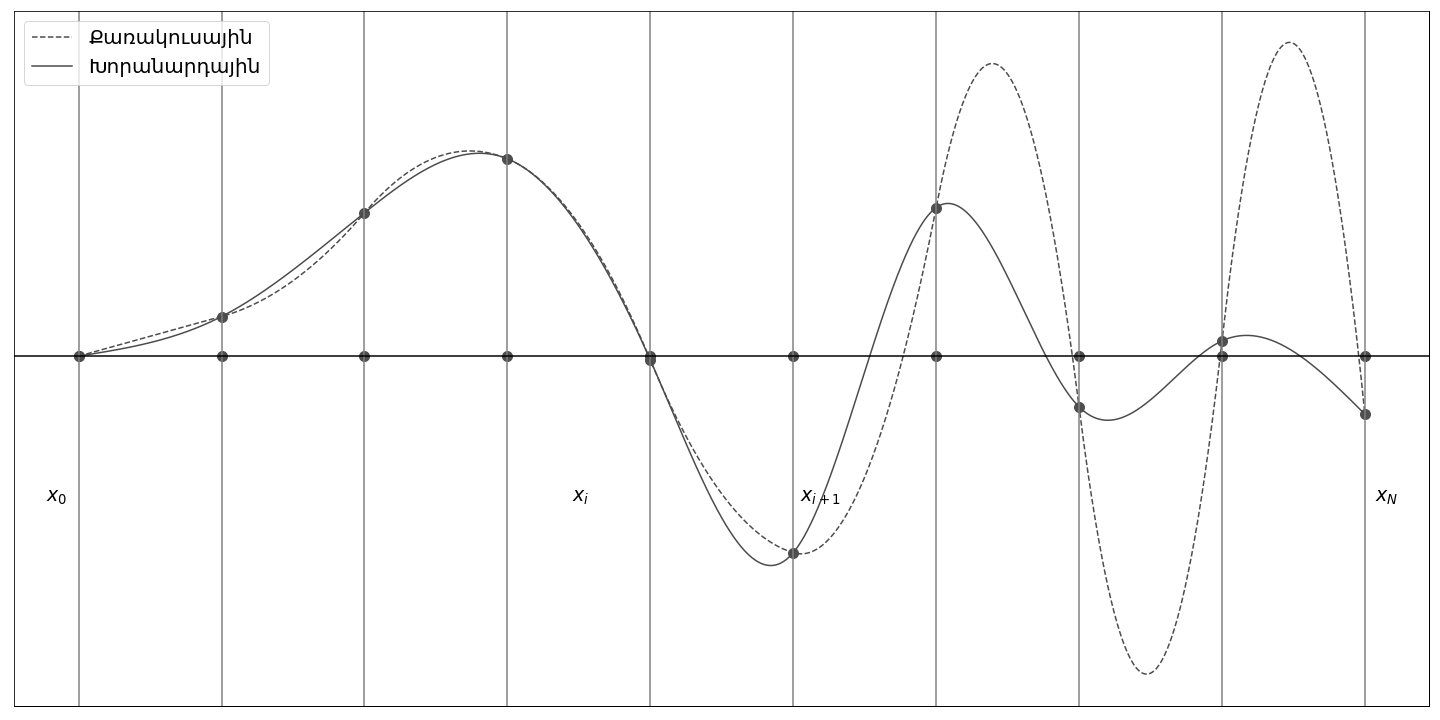
\includegraphics[width=1.0\textwidth]{images/quadratic_and_cubic_interploation}
\captionsetup{labelformat=empty}
\caption{Նկար 1.3. Քառակուսային և խորանարդային ինտերպոլյացիաների համեմատում։}
\end{figure}
\newpage
Այժմ դիտարկենք լոկալ կրող ունեցող խորանարդային սփլայները։ Այդպիսի սփլայններ առաջարկել է ավստրիացի մաթեմատիկոս Առնոլդ Շնեբերգը։
Դիտարկենք հետևյալ ֆունկցիան.
\begin{equation}
\gamma(x)=\dfrac{1}{4}\left[\left(x+2\right)^{3}_{+} - 4\left(x+1\right)^{3}_{+}+ 6\left(x\right)^{3}_{+} -4\left(x-1\right)^{3}_{+} + \left(x-2\right)^{3}_{+}\right]
\end{equation}
որտեղ
\begin{equation}
\left(x\right)_{+}=
\begin{dcases}
x, x > 0 \\
0, x \leq 0	
\end{dcases}
\end{equation}
\begin{figure}[H]
\centering
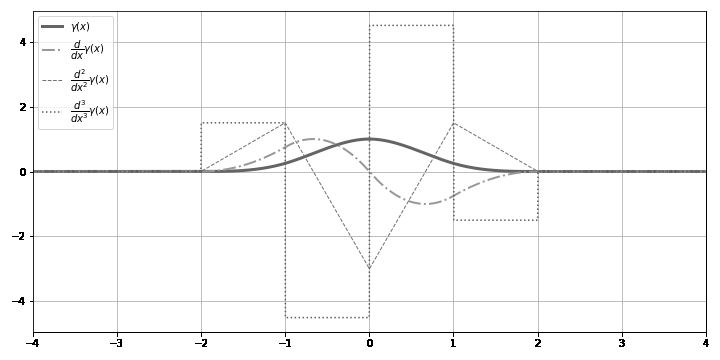
\includegraphics[width=1.0\textwidth]{images/cubic_compact_support_basis}
\captionsetup{labelformat=empty}
\caption{Նկար 1.4. $\gamma$(x) ֆունկցիան և նրա մինչև երրորդ կարգի ածանցյալները.}
\end{figure}
Ենթադրենք տրված է $\left[x_{0}, x_{N}\right]$ ինտերվալը տրոհված $N$ հավասար մասերի h քայլով։ Յուրաքանչյուր $x_{i}$ հանգույցի $(i=\overline{2, N-2})$ համար բազիսային ֆունկցիան տրվում է հետևյալ բանաձևով.
\begin{equation}
B_{i}\left(\dfrac{x}{h}\right)=\gamma \left(\frac{x-x_{0}}{h}-i\right)
\end{equation}
Այս ֆունկցիաները և նրանց մինչև երկրորդ կարգի ածանցյալները հավասար են զրոյի $\mathbb{R} \textbackslash \left(x_{i-2}, x_{i+2}\right)$ տիրույթում։
Մնացած բազիսային ֆունկիաները պետք է կառուցել այլ կերպ, քանի որ դրանց մի մասը դուրս է ըկած  $\left[x_{0}, x_{N}\right]$ ինտերվալից։
\begin{equation}
\begin{aligned}
&B_{0}\left(\frac{x}{h}\right) = \gamma \left(\frac{x}{h}\right) + \left(\dfrac{h - x}{4h}\right)^{3}_{+} , \; x \in \left[x_{0}, x_{2}\right] \\
&B_{1}\left(\frac{x}{h}\right) = \gamma \left(\frac{x}{h}\right), \; x \in \left[x_{0}, x_{3}\right]\\
&B_{N-1}\left(\frac{x}{h}\right) = \gamma \left(\frac{x}{h}\right), \; x \in \left[x_{N-3}, x_{N}\right] \\
&B_{N}\left(\frac{x}{h}\right) = \gamma \left(\frac{x}{h}\right) + \left(\dfrac{x - (N-1)h}{4h}\right)^{3}_{+} , \; x \in \left[x_{N-2}, x_{N}\right]
\end{aligned}
\end{equation}
\begin{figure}[h!]
\centering
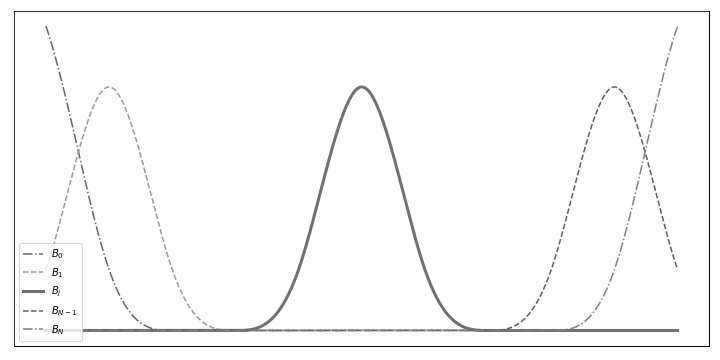
\includegraphics[width=1.0\textwidth]{images/all_cubic_compact_support_basis}
\captionsetup{labelformat=empty}
\caption{Նկար 1.5. $B_{j}$ բազիսային ֆունկցիաների գրաֆիկական ներկայացում։}
\end{figure}
Տրված $\left\{\left(x_{j}, f_{j}\right)\right\}_{j=0}^{N}$ ինտերպոլյացիոն տվյալնեով կառուցենք սփլայն.
\begin{equation}
F(x) = \sum_{i=0}^{N} \alpha_{i}B_{i}\left(\frac{x}{h}\right)$$
\end{equation}
Հաշվի առնելով ինտերպոլյացիոն պայմանները կստանանք հետևյալ հավասարումերի համակարգը.
\begin{equation}
\begin{dcases}
\frac{5}{4}\alpha_{0} + \frac{1}{4}\alpha_{0} &= f_{0}\\
\frac{1}{4}\alpha_{j-1} + \alpha_{j} + \frac{1}{4}\alpha_{j+1} &= f_{j}, \; j=\overline{1, N-1}\\
\frac{5}{4}\alpha_{N-1} + \frac{1}{4}\alpha_{N} &= f_{N}\\
\end{dcases}
\end{equation}
\newpage
\section*{\centering Գլուխ 2 \\ Երկչափ մոտարկում}
%This command resets the equation's counter 	
\setcounter{equation}{0}
Այժմ դիտարկենք երկու փոփոխականի ֆունկցիայի մոտարկման խնդիրը: Ի տարբերություն մեկ փոփոխականի ֆունկիցայի ինտերպոլյացիայի, այս դեպքում տիրույթի տրոհումը կարելի է իրականացնել կամայական ձևով։ Կախված տրված տիրույթի և տրոհման ձևից, առանձնացվում են հետևյալ մոտակման ձևերը.
\subsection*{2.1 Ուղղանկյուն տիրույթ}
Դիցուք տրված են $f:\Omega\mapsto \Theta$,  $\Theta \subset \mathbb{R}$, $\Omega \subset \mathbb{R}^{2} = \left[x_{0}, x_{M}\right] \times \left[y_{0}, y_{N}\right]$  ուղղանկյուն տիրույթը, որը տրոհված է $\left[x_{i}, x_{i+1}\right] \times \left[y_{j}, y_{j+1}\right]$, ուղղանկյուն էլեմենտների:
$$x_{i+1}-x_{i}=h_{1}, \; y_{j+1}-y_{j}=h_{2}, \; i=\overline{0, M-1}, j=\overline{0, N-1}$$
\begin{figure}[h!]
\centering
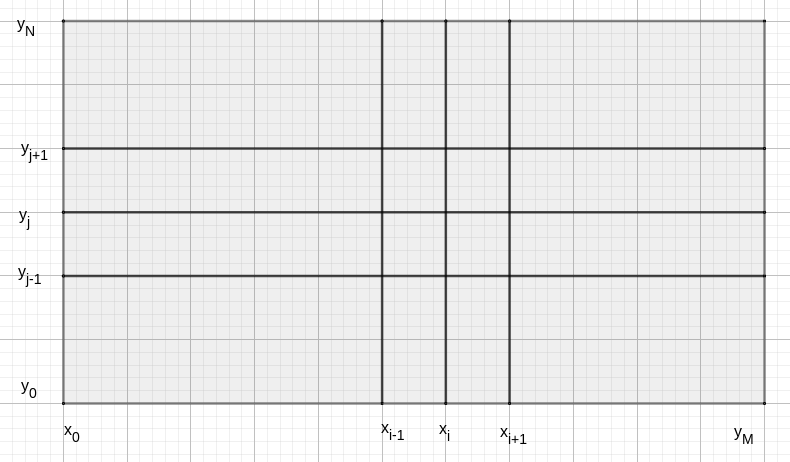
\includegraphics[width=0.6\textwidth]{images/two_var_linear}
\captionsetup{labelformat=empty}
\caption{Նկար 2.1. Ուղղանկյունաձև տիրույթի տրոհում ուղղանկյուն էլեմենտների։}
\end{figure}
\newpage
\subsubsection*{2.1.Էրմիթյան ինտերպոլյացիա}
Երկգծային ինտերպոլյացիա։

Յուրաքանչյուր  $\left[x_{i}, x_{i+1}\right] \times \left[y_{j}, y_{j+1}\right]$ էլեմենտի վրա $f$ ֆունկցիան մոտարկվում է հետևյալ քառակուսային ֆունկցիայով։
\begin{equation}
\scalemath{0.9}{p_{1}^{(i, j)}(x, y)=\alpha_{i,j}(x,y)f(x_{i},y_{j})+\beta_{i+1,j}(x,y)f(x_{i+1},y_{j})\scalemath{0.2}+\gamma_{i,j+1}(x,y) f(x_{i},y_{j+1})+\delta_{i+1, j+1}(x,y)f(x_{i+1},y_{j+1})}
\end{equation}
որտեղ 
\begin{equation}
\begin{aligned}
&\alpha_{i,j}(x,y)=\dfrac{1}{h_{1}h_{2}}\left(x_{i+1}-x\right)\left(y_{j+1}-y\right) \\
&\beta_{i+1,j}(x,y)=\dfrac{1}{h_{1}h_{2}}\left(x-x_{i}\right)\left(y_{j+1}-y\right) \\
&\gamma_{i,j+1}(x,y)=\dfrac{1}{h_{1}h_{2}}\left(x_{i+1}-x\right)\left(y-y_{j}\right) \\
&\delta_{i+,j+1}(x,y)=\dfrac{1}{h_{1}h_{2}}\left(x-x_{i}\right)\left(y-y_{j}\right)
\end{aligned}
\end{equation}
Այսպիսով $\left[x_{0}, x_{M}\right] \times \left[y_{0}, y_{M}\right]$ տիրույթում կտոր առ կտոր մոտարկող ֆունկցիան տրվում է հետևյալ բանաձևով.
\begin{equation}
p_{1}(x,y)=\sum_{i=0}^{M}\sum_{j=0}^{N}\varphi_{i,j}(x,y)f(x_{i},y_{j})
\end{equation}
որտեղ
\begin{equation}
\varphi_{i,j}\left(x, y\right)=\begin{dcases}
\dfrac{1}{h_{1}h_{2}}\left(x-x_{i-1}\right)\left(y-y_{j-1}\right), (x,y)\in \left[x_{i-1}, x_{i}\right]\times\left[y_{j-1}, y_{j}\right]\\
\dfrac{1}{h_{1}h_{2}}\left(x-x_{i-1}\right)\left(y_{j+1}-y\right), (x,y)\in \left[x_{i-1}, x_{i}\right]\times\left[y_{j}, y_{j+1}\right]\\
\dfrac{1}{h_{1}h_{2}}\left(x_{i+1}-x\right)\left(y-y_{j-1}\right), (x,y)\in \left[x_{i}, x_{i+1}\right]\times\left[y_{j-1}, y_{j}\right]\\
\dfrac{1}{h_{1}h_{2}}\left(x_{i+1}-x\right)\left(y_{j+1}-y\right), (x,y)\in \left[x_{i}, x_{i+1}\right]\times\left[y_{j}, y_{j+1}\right]\\
0, \text{մնացած դեպքերում}
\end{dcases}
\end{equation}

\newpage 

Երկխորանարդային ինտերպոլյացիա։

Միավոր քառակուսու վրա կառուցենք մոտարկող ֆունկցիա, որը լրիվ խորանարդային բազմանդամ է ըստ երկու փոփոխականի.

\begin{equation}
			p_{3}^{(i, j)}(x, y)=\sum_{i, j=0}^{3}\alpha_{ij}x^{i}y^{j}
\end{equation}

որտեղ $\alpha_{ij}$ գործակիցները միարժեքորեն որոշվում են $f, \dfrac{\partial f}{\partial x}, \dfrac{\partial f}{\partial y}, \dfrac{\partial^{2} f}{\partial x \partial y}$ ֆունկցիաների արժեքներով գագաթների վրա։ Դրանք որոշելով $\left(5\right)$ գումարը կարող ենք ներկայացնել հետևյալ տեսքով.

\begin{equation}
			p_{3}^{(i, j)}(x, y)= \mathlarger{\sum_{0 \leq i, j, k, l \leq 1}} \dfrac{\partial^{k+l}}{\partial x^{k} \partial y^{l}}  \psi_{i}^{(k)}(x)\psi_{j}^{(l)}(y)
\end{equation}
որտեղ
\begin{equation*}
\begin{aligned}
&\psi_{0}^{(0)}(t) = \left(1-t\right)^{2}\left(1+2t\right) \\
&\psi_{0}^{(1)}(t) = \left(1-t\right)^{2}t \\
&\psi_{1}^{(0)}(t) = t^{2}\left(3-2t\right) \\
&\psi_{1}^{(1)}(t) = t^{2}\left(t-1\right) \\
\end{aligned}
\end{equation*}
Այժմ օգտվելով $\left(5\right)$ բանաձևից և ունենալով տրված տիրույթի տրոհման $h_{1}$ և $h_{2}$ քայլերը, յուրաքանչյուր գագաթի համար կարող ենք կազմել բազիսային ֆունկցիա, և ամբող տիրույթում ինտերպոլացնող ֆունկցիան կունենա հետևյալ տեսքը.
\begin{equation}
\scalemath{0.70}{
p_{3}(x)=\sum_{i=0}^{M}\sum_{j=0}^{N}\left[f_{ij}\varphi^{(0)}\left(\frac{x}{h_{1}}\right)\varphi^{(0)}\left(\frac{y}{h_{2}}\right)+\dfrac{\partial f_{ij}}{\partial x}\varphi^{(1)}\left(\frac{x}{h_{1}}\right)\varphi^{(0)}\left(\frac{y}{h_{2}}\right) +\dfrac{\partial f_{ij}}{\partial y}\varphi^{(0)}\left(\frac{x}{h_{1}}\right)\varphi^{(1)}\left(\frac{y}{h_{2}}\right) +\dfrac{\partial^{2} f_{ij}}{\partial x\partial y}\varphi^{(1)}\left(\frac{x}{h_{1}}\right)\varphi^{(1)}\left(\frac{y}{h_{2}}\right)\right]}
\end{equation}

որտեղ

\begin{equation}
\begin{aligned}
&\varphi^{(0)}=\begin{dcases}
\left(1+t\right)^{2}\left(1-2t\right), \; -1\leq x \leq 0 \\
\left(1-t\right)^{2}\left(1+2t\right), \; 0\leq  x \leq  1 \\
\end{dcases}
\\
&\varphi^{(1)}=\begin{dcases}
\left(1+t\right)^{2}t, \; -1\leq  x \leq 0 \\
\left(1-t\right)^{2}t, \; 0\leq  x \leq 1 \\
\end{dcases}
\end{aligned}
\end{equation}

\begin{figure}[H]
  \centering
  \begin{minipage}[b]{0.45\textwidth}
    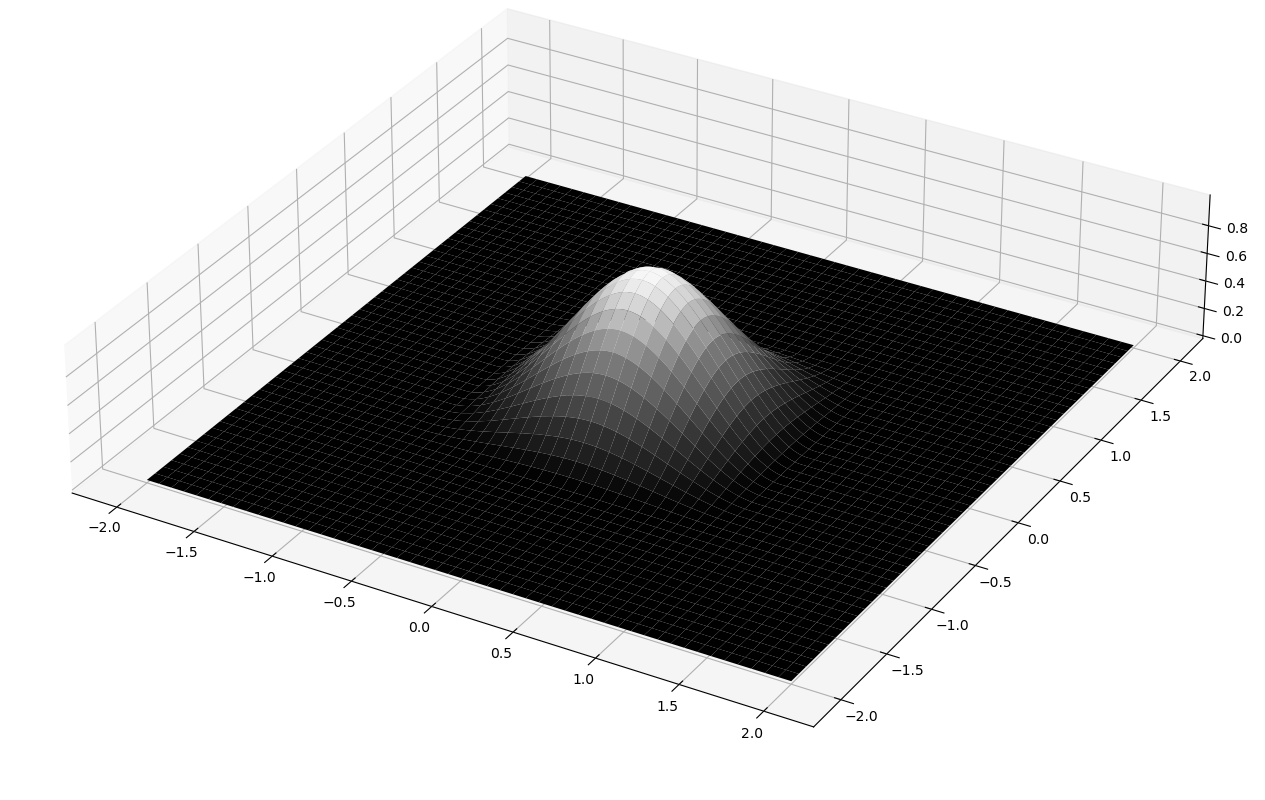
\includegraphics[width=\textwidth]{images/two_dimensional_ermite_1}
    %\captionsetup{labelformat=empty}
  \end{minipage}
  \hfill
  \begin{minipage}[b]{0.45\textwidth}
    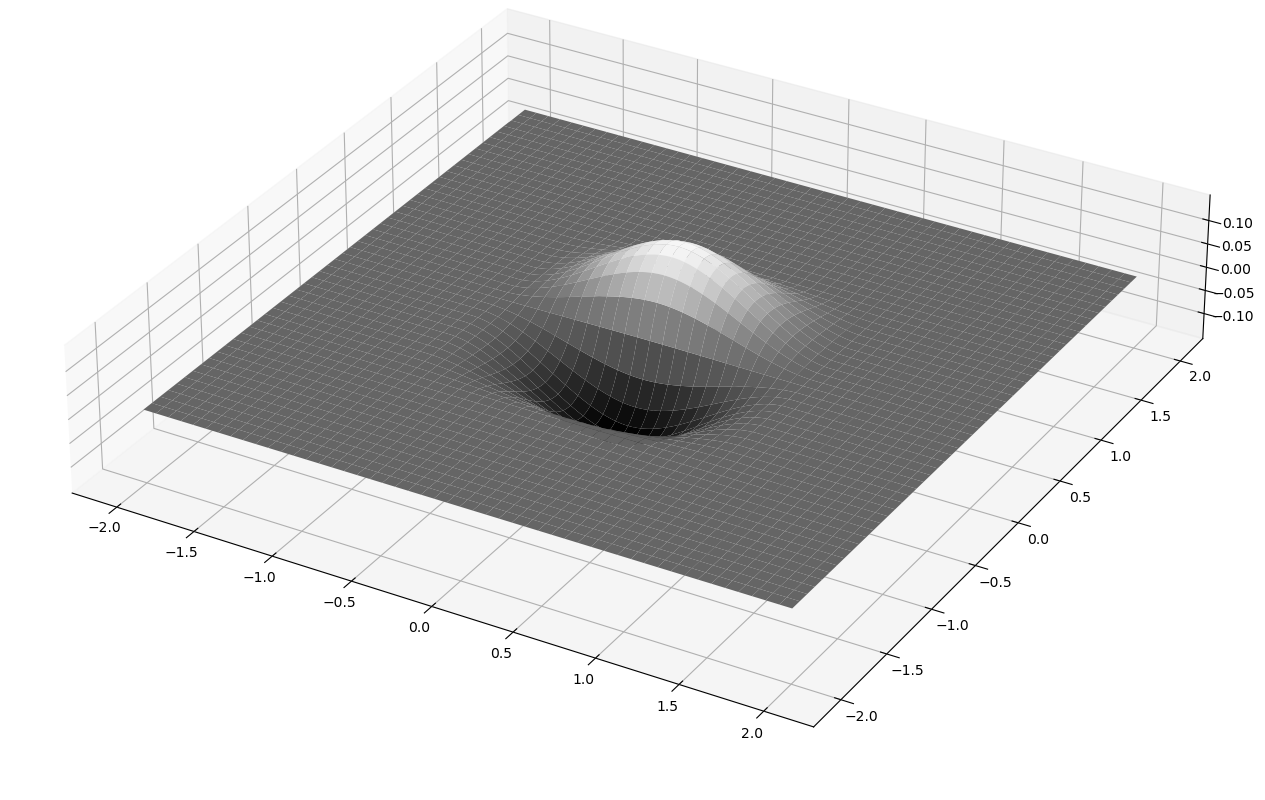
\includegraphics[width=\textwidth]{images/two_dimensional_ermite_2}
    %\captionsetup{labelformat=empty}
  \end{minipage}
\\
  \begin{minipage}[b]{0.45\textwidth}
    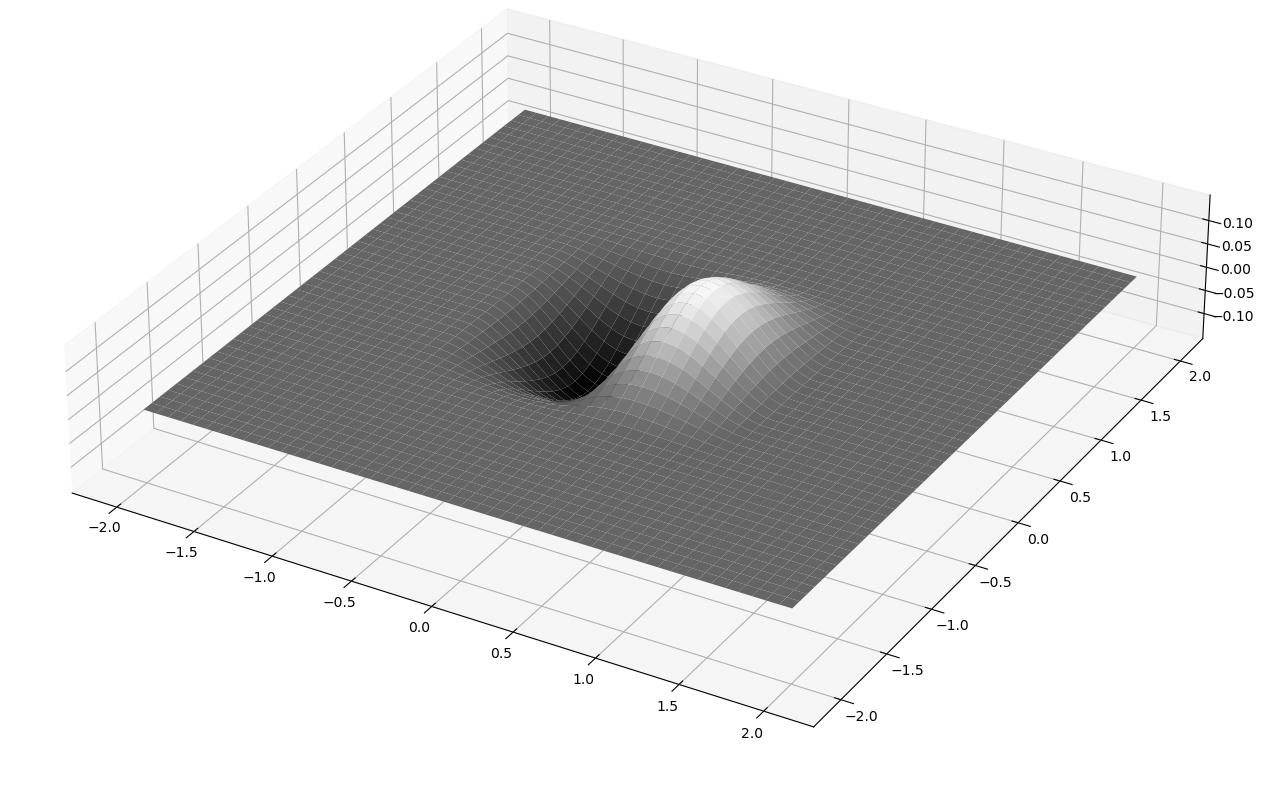
\includegraphics[width=\textwidth]{images/two_dimensional_ermite_3}
    %\captionsetup{labelformat=empty}
  \end{minipage}
\hfill
  \begin{minipage}[b]{0.45\textwidth}
    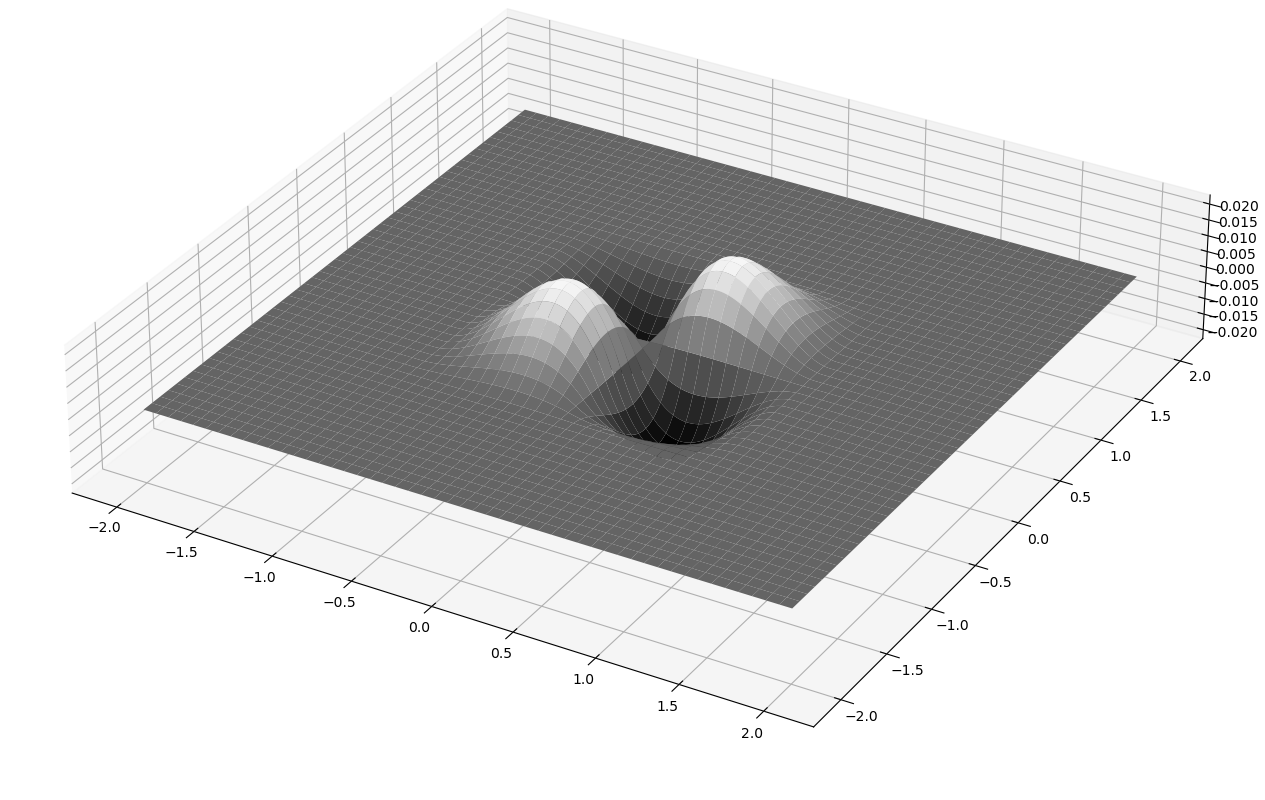
\includegraphics[width=\textwidth]{images/two_dimensional_ermite_4}
    %\captionsetup{labelformat=empty}
  \end{minipage}
\captionsetup{labelformat=empty}
\caption{Նկար 2.2 Երկխորանարդային ինտերպոլյացիայի բազիսային ֆունկցիաների գծապատկեր։}
\end{figure}

Վերը ներկայացված երկու ինտերպոլյացիաները էրմիթյան ինտերպոլյացիայի մասնովոր դեպքեր են։
Ընդհանուր դեպքում ցանկացած $k$ բնական թվի և տրված ուղղանկյունաձև տրոհման յուրաքանչյուր էլեմենտի վրա կարելի է կառուցել $C^{\left(k-1, k-1\right)}$ ինտերպոլացնող ֆունկցիա, որը ըստ յուրաքանչյուր փոփոխականի $\left(2k-1\right)$֊րդ կարգի բազմանդամ է և բավարարում է հետևյալ պայմաններին.
\begin{equation}
\dfrac{\partial^{p+q}}{\partial x^{p} \partial x^{q}}f\left(x_{i}, y_{j}\right)=\dfrac{\partial^{p+q}}{\partial x^{p} \partial x^{q}}p_{2k-1}\left(x_{i}, y_{j}\right), \; p,q=\overline{0, k-1}, \;  i=\overline{0, M}, \; j=\overline{0, N}
\end{equation}

\noindent Գծային ինտերպոլյացիա։

Այժմ դիտարկենք ուղղանկյուն տիրույթի տրոհման և բազիսային ֆունկցիաների կառուցման այլ տարբերակ։ Այս դեպքում տիրույթը տրոհենք ինչպես նախորդ դեպքում, ի հավելումն յուրաքանչյուր ուղղանկյուն էլեմենտ տրոհելով երկու ուղղանկյուն եռանկյունների, ինչպես ցույց է տրված Նկար 2.2-ում։
Դիտարկենք հետևյալ ֆունկցիան.
\begin{equation}
$$\varphi \left(x,y\right)=\begin{cases}
1-y, &(x,y) \in S_{1} \\
1+x-y, &(x,y) \in S_{2} \\
1+x, &(x,y) \in S_{3} \\
1+y, &(x,y) \in S_{4} \\
1-x+y, &(x,y) \in S_{5} \\
1-x, &(x,y) \in S_{6}\\
0, \text{մնացած դեպքերում}\\
\end{cases}
\end{equation}
\begin{figure}[H]
  \centering
  \begin{minipage}[b]{0.4\textwidth}
    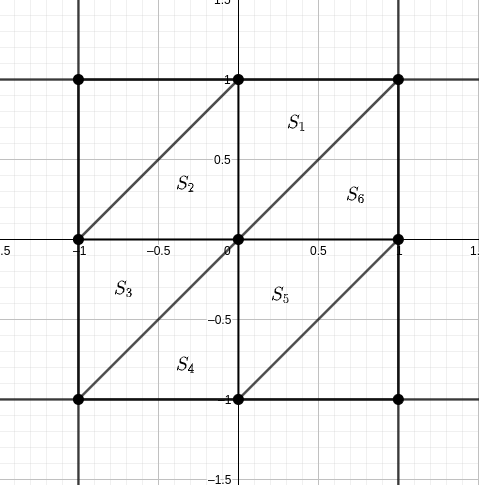
\includegraphics[width=\textwidth]{images/two_var_courant_1}
    \captionsetup{labelformat=empty}
    \caption{Նկար 2.3. Ուղղանկյուն էլեմենտի տրոհումը եռանկյունների։}
  \end{minipage}
  \hfill
  \begin{minipage}[b]{0.4\textwidth}
    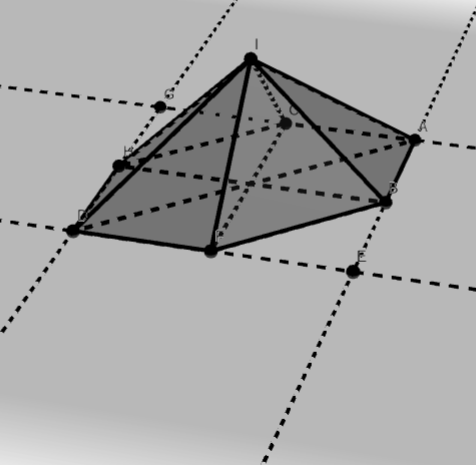
\includegraphics[width=\textwidth]{images/two_var_courant_2}
    \captionsetup{labelformat=empty}
    \caption{Նկար 2.4. Բազիսային ֆունկցիայի տեսքը}
  \end{minipage}
\end{figure}
Պարզ է, որ այն $\left[-1, 1\right] \times \left[-1	, 1\right]$ տիրույթում $C^{(0, 0)}$ ֆունկցիա է: Այն հայտնի է որպես Կուրանտի բազիսային ֆունկցիա, ի պատիվ գերմանացի մաթեմատիկոս Ռիխարդ Կուրանտի։
Այժմ յուրաքանչյուր $\left(x_{i}, y_{j}\right)$ հանգուցային կետի համար կառուցենք բազիսային ֆունկցիա օգտվելով $\left(6\right)$-ից.
\begin{equation}
\varphi^{(ij)}(x,y)=\varphi \left(\dfrac{x-x_{i}}{h_{1}}, \dfrac{y-y_{j}}{h_{2}}\right)
\end{equation}
Յուրաքանչյուր կետի համար ունենալով բազիսային ֆունկցիա, $f$ ֆունկցիայի մոտարկման բանաձևը կտվրի հետևյալ կերպ.
\begin{equation}
p_{1}(x,y)=\sum_{i=0}^{N}\sum_{j=0}^{M}\varphi^{(ij)}(x,y)f(x_{i}, y_{j})
\end{equation}
\begin{figure}[H]
\centering
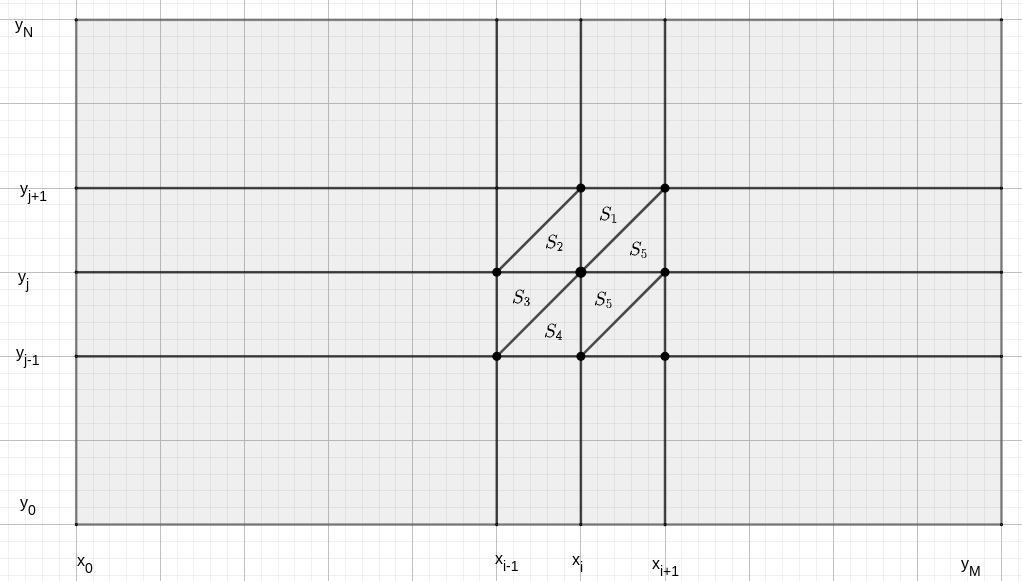
\includegraphics[width=0.6\textwidth]{images/two_var_courant_3}
\captionsetup{labelformat=empty}
\caption{Նկար 2.5. Տիրույթի տրոհումը ուղղանկյուն եռանկյունների}
\end{figure}
\newpage
\subsubsection*{2.2. Խորանարդային մոտարկում}

Երկխորանարդային սփլայն։

Մեկ փոփոխականի մոտարկան խնդրը դիտարկելից քննարկեցինք Շներբերգի կողմից առաջարկված խորանարդային բազիսային սփլայնները։ Այս սփլայնները կարող ենք  օգտագործել երկչափ մոտարկման համար։
Յուրաքանչյուր $\left(x_{i}, y_{j}\right)$ հանգույցի վրա կառուցենք բազիսային ֆունկցիա կազմելով $B_{i}\left(\dfrac{x}{h_{1}}\right)$ և $B_{j}\left(\dfrac{x}{h_{2}}\right)$ ֆունկցիաների թենզորական  արտադրյալը։
\begin{equation}
\varphi^{(ij)}\left(x, y\right) = B_{i}\left(\dfrac{x}{h_{1}}\right) B_{j}\left(\dfrac{x}{h_{2}}\right)$$
\end{equation}
\noindent Տրված $\left\{\left(x_{ij}, y_{ij}, f_{ij}\right)\right\}$ ինտերպոլյացիոն տվյալնեով կառուցենք սփլայն.
\begin{equation}
F(x,y) = \sum_{i=0}^{N} \alpha_{ij}\varphi^{(ij)}\left(x, y\right)$$
\end{equation}
Հաշվի առնելով ինտերպոլյացիոն պայմանները կստանանք հետևյալ հավասարումերի համակարգը.
\begin{equation}
\begin{dcases}
\alpha_{00}+\frac{5}{16}(\alpha_{01} + \alpha_{10}) +\frac{1}{16}\alpha_{11} &= f_{00}\\
\alpha_{M0}+\frac{5}{16}(\alpha_{M1} + \alpha_{M-1,0}) +\frac{1}{16}\alpha_{M-1, 1} &= f_{M0}\\
\alpha_{0N}+\frac{5}{16}(\alpha_{1N} + \alpha_{0,N-1}) +\frac{1}{16}\alpha_{N-1, 1} &= f_{0N}\\
\alpha_{MN}+\frac{5}{16}(\alpha_{M-1,N} + \alpha_{M,N-1}) +\frac{1}{16}\alpha_{M-1,N-1} &= f_{MN}\\
\frac{5}{4}\alpha_{i,1}+\frac{5}{16}(\alpha_{i-1,0} + \alpha_{i+1,0}) +\frac{1}{4}\alpha_{i,1} + \frac{1}{16}(\alpha_{i-1,1}+\alpha_{i+1,1}) &= f_{i0}\\
\frac{5}{4}\alpha_{i,N-1}+\frac{5}{16}(\alpha_{i-1,N} + \alpha_{i+1,N}) +\frac{1}{4}\alpha_{i,N-1} + \frac{1}{16}(\alpha_{i-1,N-1}+\alpha_{i+1,N-1}) &= f_{iN}\\
\frac{5}{4}\alpha_{1,j}+\frac{5}{16}(\alpha_{0,j-1} + \alpha_{0,j+1}) +\frac{1}{4}\alpha_{1,j} + \frac{1}{16}(\alpha_{1,j-1}+\alpha_{1,j+1}) &= f_{0j}\\
\frac{5}{4}\alpha_{M-1,j}+\frac{5}{16}(\alpha_{M,j-1} + \alpha_{M,j+1}) +\frac{1}{4}\alpha_{M-1,j} + \frac{1}{16}(\alpha_{M-1,j-1}+\alpha_{M-1,j+1})& = f_{Mj}\\
\alpha_{ij} + \frac{1}{4}(\alpha_{i,j-1} + \alpha_{i,j+1} + \alpha_{i-1,j} + \alpha_{i+1,j}) + \frac{1}{16}(\alpha_{i-1,j-1} + \alpha_{i-1,j+1} + \alpha_{i+1,j-1} +\alpha_{i+1,j+1}) &= f_{ij}
\end{dcases}
\end{equation}
\newpage
\begin{figure}[h!]
\centering
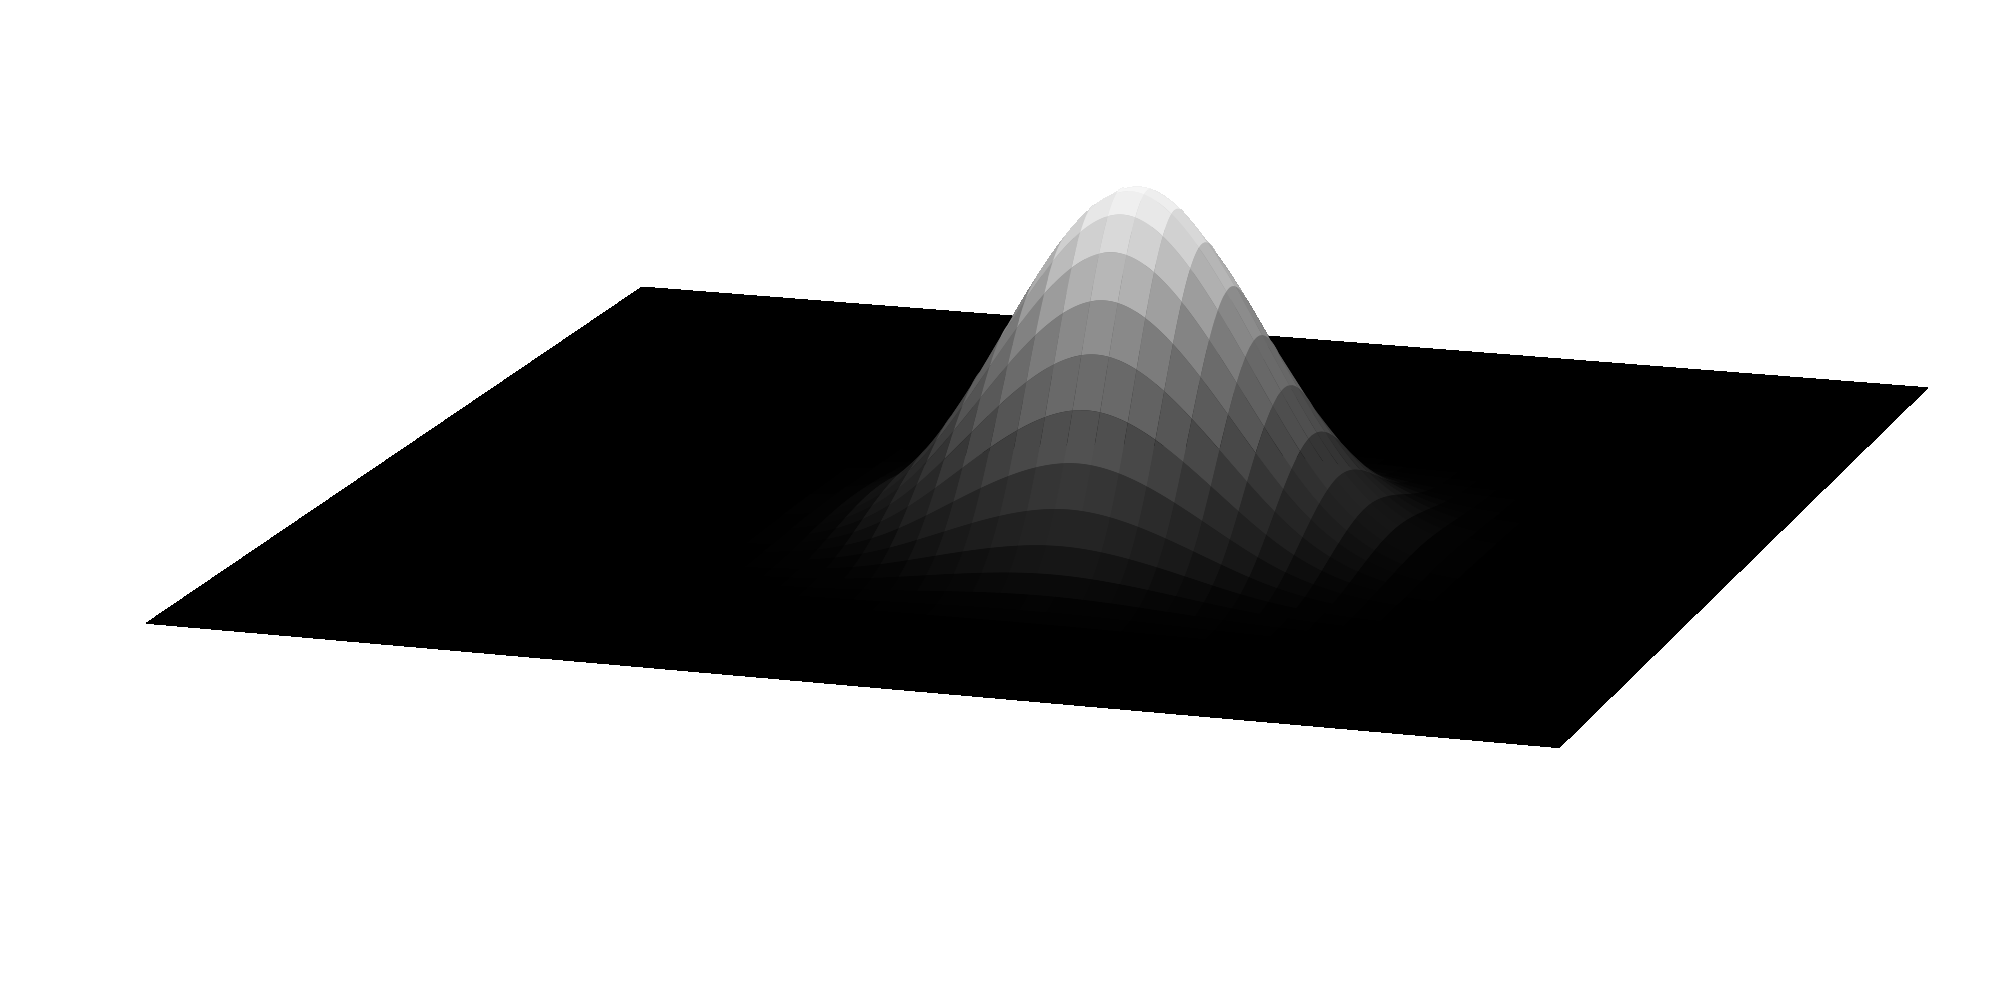
\includegraphics[width=1.0\textwidth]{images/two_dimensional_basis}
\captionsetup{labelformat=empty}
\caption{Նկար 2.6. $\varphi^{ij}$ բազիսային ֆունկցիաների պատկեր։}
\end{figure}
\begin{figure}[h!]
\centering
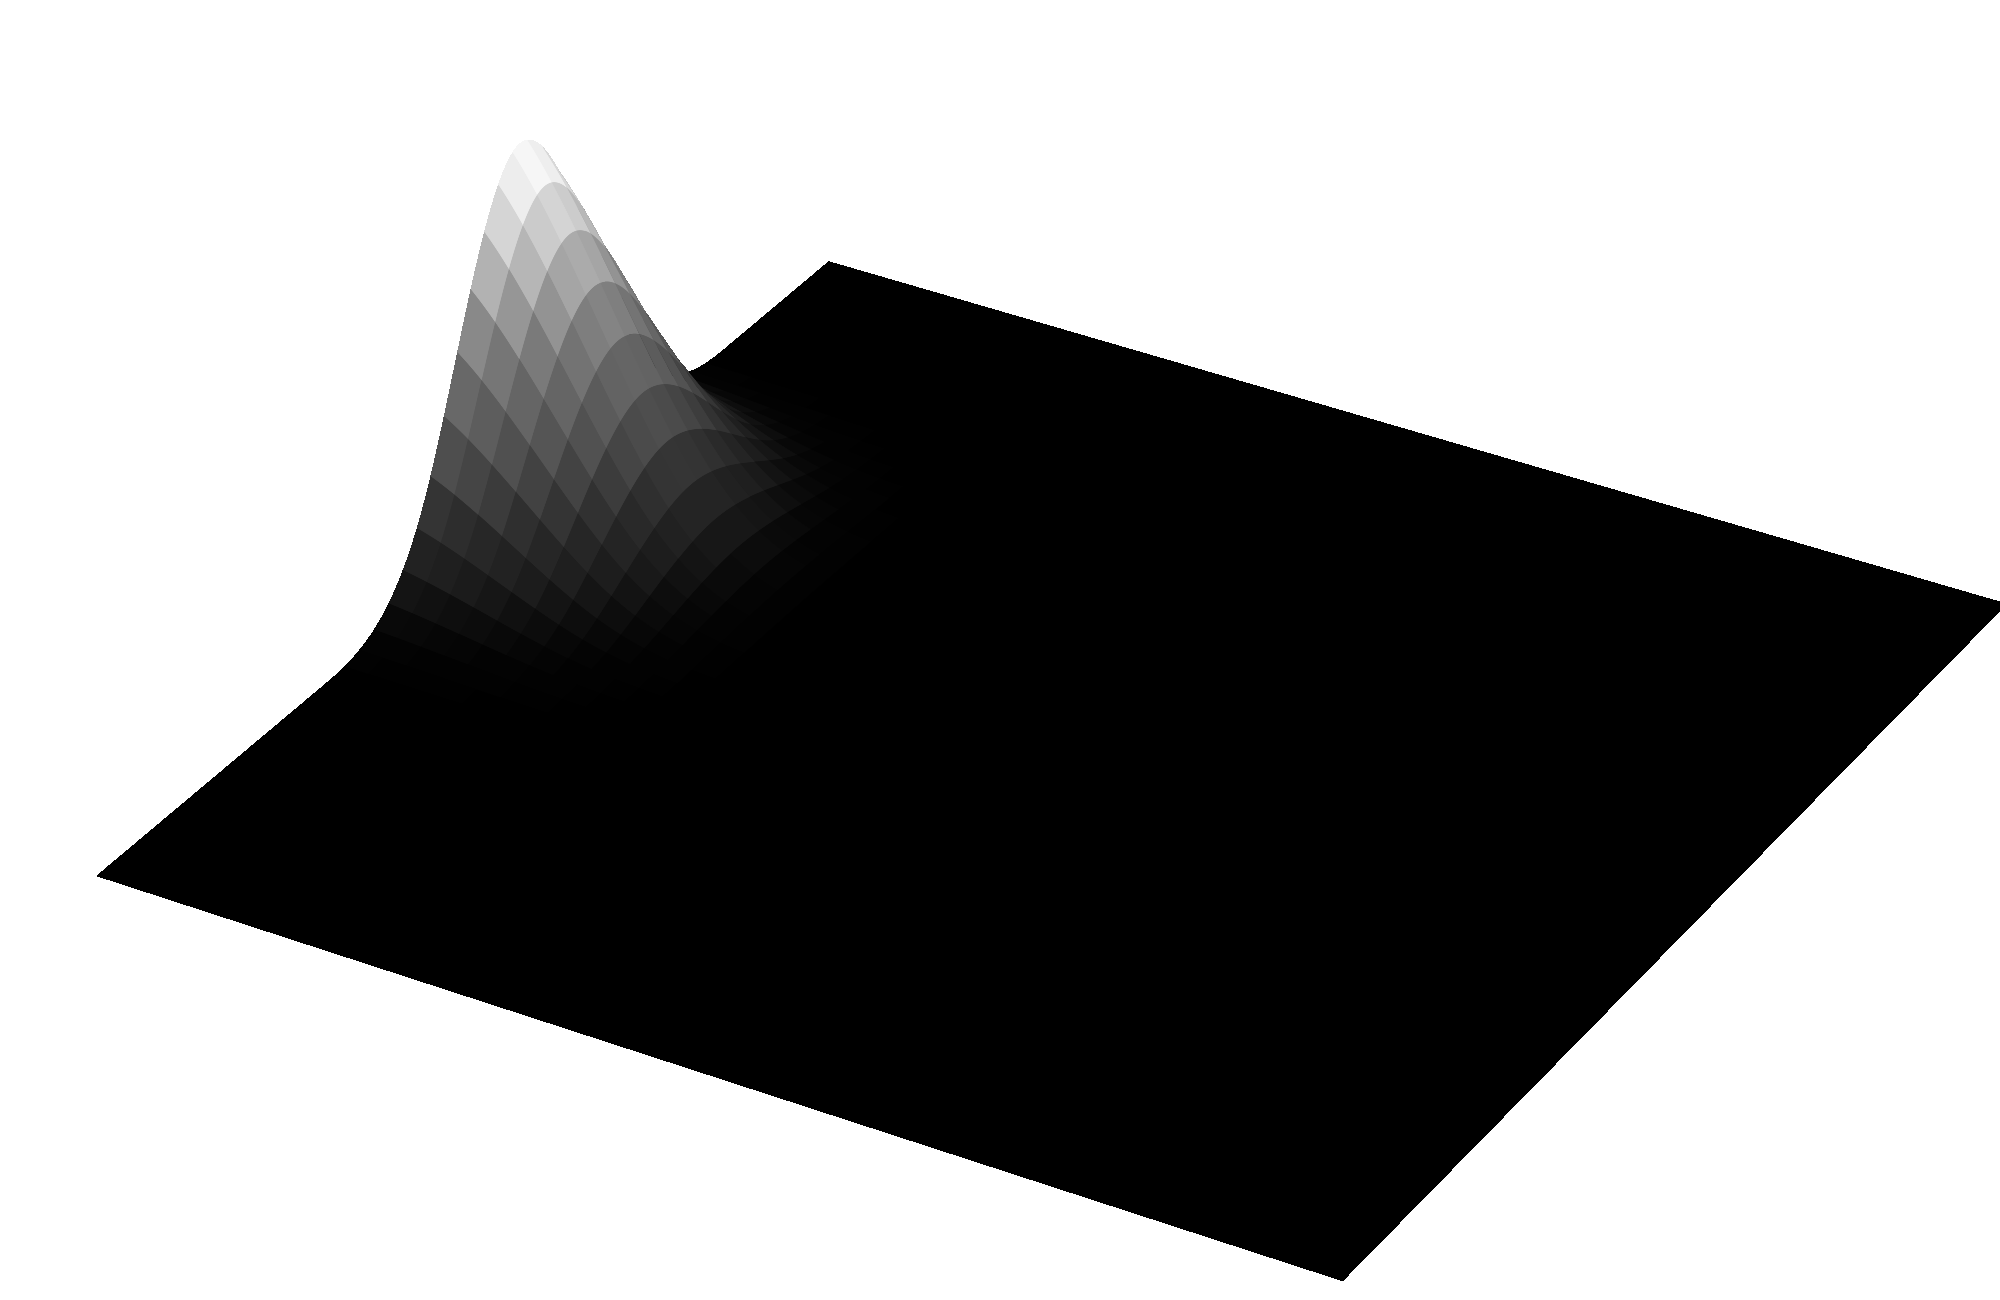
\includegraphics[width=1.0\textwidth]{images/two_dimensional_basis_1}
\captionsetup{labelformat=empty}
\caption{Նկար 2.7 Տիրույթի եզրի վրա գտնվող բազիսային ֆունկցիա։}
\end{figure}
\newpage
\subsection*{Բազմանկյուն տիրույթ}
Բազմանկյուն տիրույթ ասելով կհասկանանք կամ հենց բազմանկյունաձև տիրույթը, կամ դրա բազմանկյուններով մոտարկումը։
Դիցուք տրված են $f:\Omega\mapsto \Theta, \Theta \subset \mathbb{R}, \Omega \subset \mathbb{R}^{2} $ բազմանկյուն տիրույթը, որը կամայական ձևով տրոհված է եռանկյուն էլեմենտների։
\begin{figure}[H]
\centering
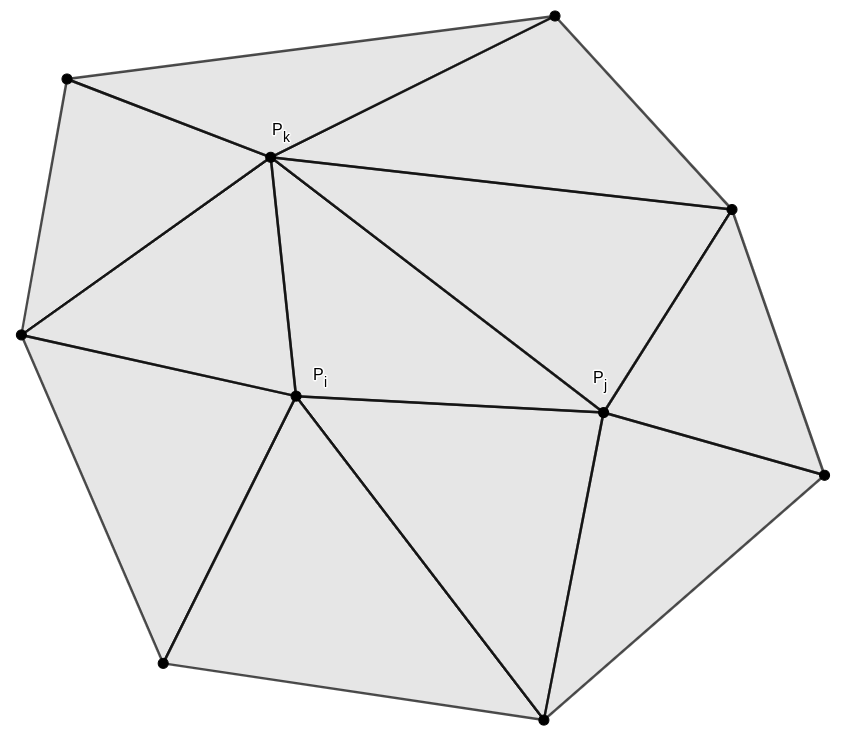
\includegraphics[width=0.4\textwidth]{images/two_var_triangular}
\captionsetup{labelformat=empty}
\caption{Նկար 2.8. Տիրույթի եռանկյունաձև տրոհման օրինակ։}
\end{figure}
\subsubsection*{2.2 Լագրանժի ինտերպոլյացիա}
Յուրաքանչուր եռանկյուն էլեմենտի վրա դիտարկենք $m$֊րդ կարգի լրիվ բազմանդամ
\begin{equation}
				F_{m}\left(x,y\right)=\sum_{k+l=0}^{m}\alpha_{kl}x^{k}y^{l}
\end{equation}
որը կարող է օգտագործվել որպես ինտերպոլյացիոն ֆունկցիա $\dfrac{1}{2}\left(m+1\right)\left(m+2\right)$ սիմետրիկ դասավորված կետերի վրա։
Դիտարկենք հետևյալ մասնավոր դեպքերը.
\begin{enumerate}
\item{Գծային ինտերպոլյացիա (m=1)}

Յուրաքանչյուր $P_{1}, P_{2}, P_{3}$ գագաթներով եռանկյուն էլեմենտի համար դիտարկենք հետևյալ մոտարկող ֆունկցիան.
\begin{equation}
F_{1}(x, y) = \dfrac{1}{S}\sum_{i=1}^{3} p^{(1)}_{i}(x,y)f(x_{i}, y_{i})
\end{equation}
որտեղ $S$֊ը $P_{1}, P_{2}, P_{3}$ կետերով կազմված եռանկյան մակերեսի կրկնապատիկն է, իսկ $p^{(1)}_{i}$ ֆունկցիաները սահմանվում են հետևյալ կերպ.


$$S = \begin{vmatrix}
     1 & x_1 & y_1\\ 
     1 & x_2 & y_2\\
     1 & x_3 & y_3 
\end{vmatrix}$$
\begin{equation}
p^{(1)}_{i}(x,y) = x_{j}y_{k}-x_{k}y_{j}+x(y_{j}-y_{k})-y(x_{j}-x_{k})
\end{equation}
որտեղ $(x_{i}, y_{i}), \; i=1, 2, 3$ տրված եռանկյուն էլեմենտի գագաթներն են (հերթականությունը ժամսլաքին հակառակ ուղղությամբ)։
\item{Քառակուսային ինտերպոլյացիա (m=2)}

Յուրաքանչյուր եռանկյուն էլեմենտի վրա գագաթներից բացի դիտարկենք նաև միջնակետերը։ Ինտերպոլացնող բազմանդամը ունի հետևյալ տեսքը.
\begin{equation}
F_{2}(x, y) = \dfrac{1}{S^{2}}\sum_{i=1}^{6} p^{(2)}_{i}(x,y)f(x_{i}, y_{i})
\end{equation}
որտեղ 
\begin{equation}
\begin{aligned}
&p^{(2)}_{i}(x,y) = p^{(1)}_{i}(x,y)\left(2 p^{(1)}_{i}(x,y)-1\right), \; i = 1, 2, 3 \\
&p^{(2)}_{4}(x,y) =  4p^{(1)}_{1}(x,y)p^{(1)}_{2}(x,y) \\
&p^{(2)}_{5}(x,y) =  4p^{(1)}_{2}(x,y)p^{(1)}_{3}(x,y) \\
&p^{(2)}_{6}(x,y) =  4p^{(1)}_{1}(x,y)p^{(1)}_{3}(x,y)
\end{aligned}
\end{equation}
\begin{figure}[H]
\centering
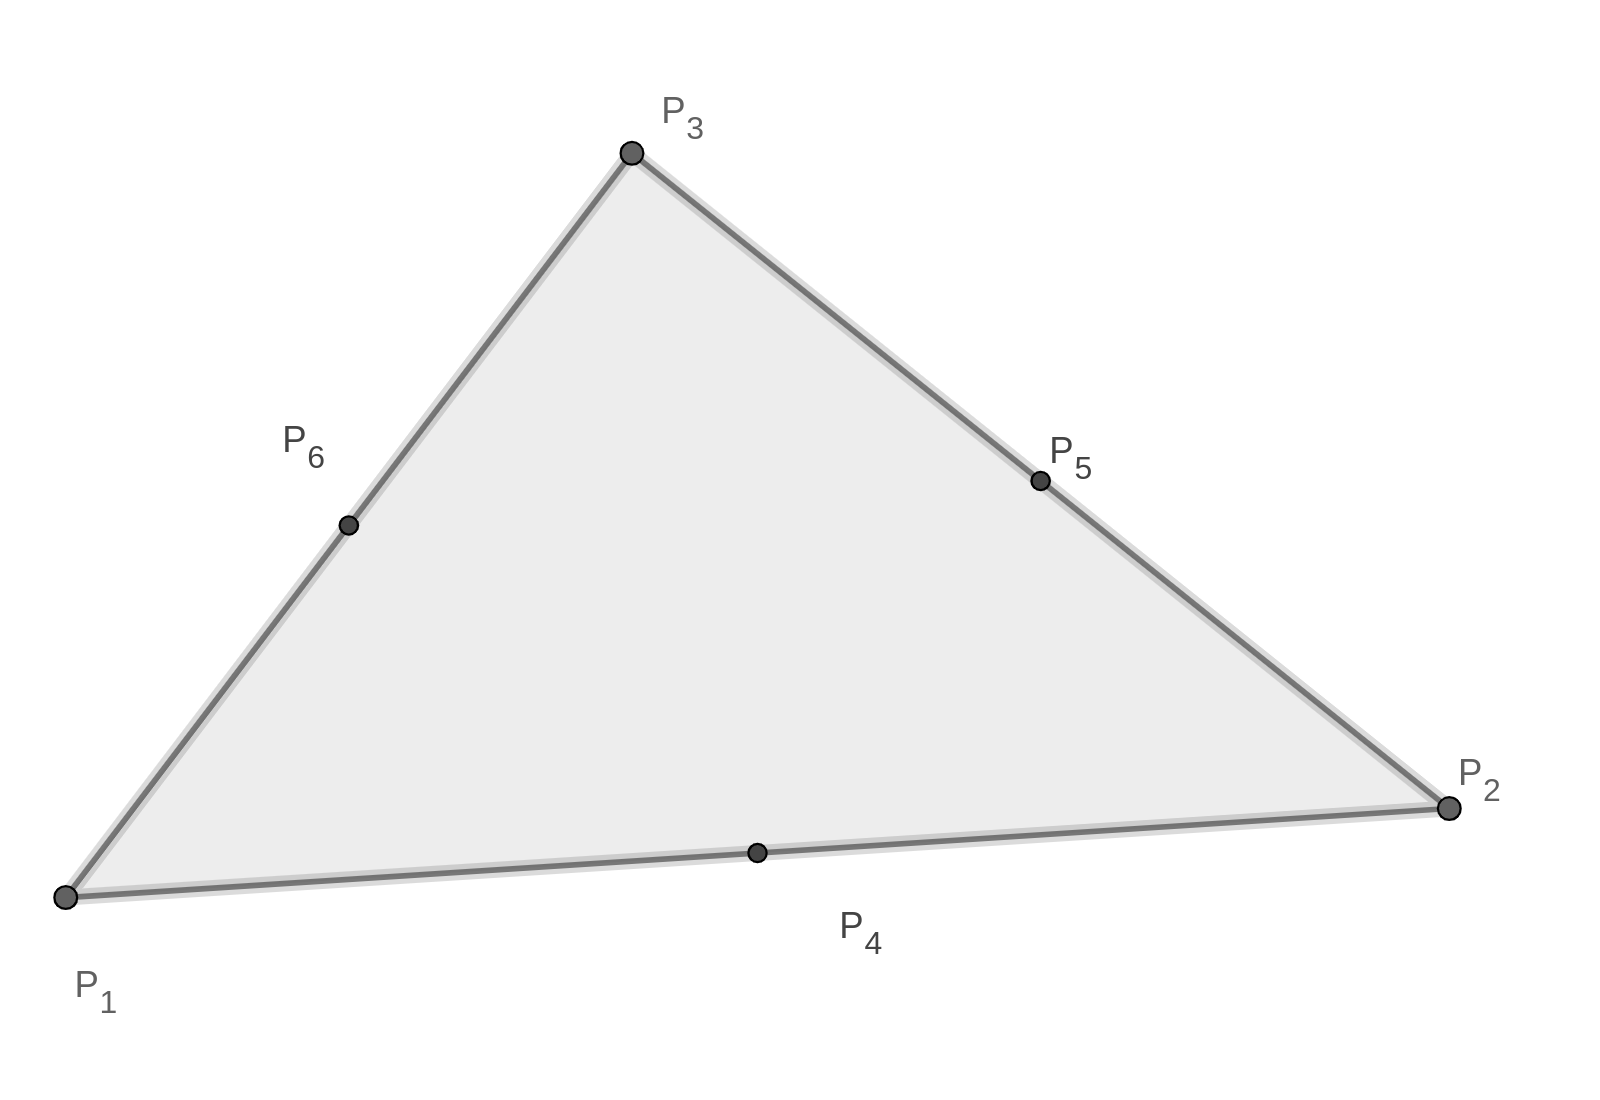
\includegraphics[width=0.4\textwidth]{images/quadratic_on_triangular}
\captionsetup{labelformat=empty}
\caption{Նկար 2.8. Կետերի դասավորվածությունը կամայական եռանկյան վրա։}
\end{figure}
\item{Խորանարդային ինտերպոլյացիա (m=3)}

Այս տեպքում յուրականչյուր կողի վրա ավելացնենք ևս երկու կետ այն տրոհելով երեք հավասար մասի  և դրանց ավելացնելով եռանկյան կենտրոնը։ Ինտերպոլացնող բազմանդամը ունի հետևյալ տեսքը.
\begin{equation}
F_{3}(x, y) = \dfrac{1}{S^{3}}\sum_{i=1}^{10} p^{(3)}_{i}(x,y)f(x_{i}, y_{i})
\end{equation}
որտեղ 
\begin{equation}
\begin{aligned}
&p^{(3)}_{i}(x,y) =  \dfrac{1}{2}p^{(1)}_{i}(x,y)\left(3 p^{(1)}_{i}(x,y)-1\right)\left(3 p^{(1)}_{i}(x,y)-2\right), \; i = 1, 2, 3 \\
&p^{(3)}_{4}(x,y) =  \dfrac{9}{2}p^{(1)}_{1}(x,y) p^{(1)}_{2}(x,y)\left(3 p^{(1)}_{1}(x,y)-1\right)\\
&p^{(3)}_{5}(x,y) =  \dfrac{9}{2}p^{(1)}_{1}(x,y) p^{(1)}_{2}(x,y)\left(3 p^{(1)}_{2}(x,y)-1\right)\\
&p^{(3)}_{6}(x,y) =  \dfrac{9}{2}p^{(1)}_{2}(x,y) p^{(1)}_{3}(x,y)\left(3 p^{(1)}_{3}(x,y)-1\right)\\
&p^{(3)}_{7}(x,y) =  \dfrac{9}{2}p^{(1)}_{2}(x,y) p^{(1)}_{3}(x,y)\left(3 p^{(1)}_{3}(x,y)-1\right) \\
&p^{(3)}_{8}(x,y) =  \dfrac{9}{2}p^{(1)}_{3}(x,y) p^{(1)}_{1}(x,y)\left(3 p^{(1)}_{3}(x,y)-1\right)\\
&p^{(3)}_{9}(x,y) =  \dfrac{9}{2}p^{(1)}_{3}(x,y) p^{(1)}_{1}(x,y)\left(3 p^{(1)}_{1}(x,y)-1\right) \\
&p^{(3)}_{10}(x,y) = 27p^{(1)}_{1}(x,y)p^{(1)}_{2}(x,y)p^{(1)}_{3}(x,y)
\end{aligned}
\end{equation}

\begin{figure}[H]
\centering
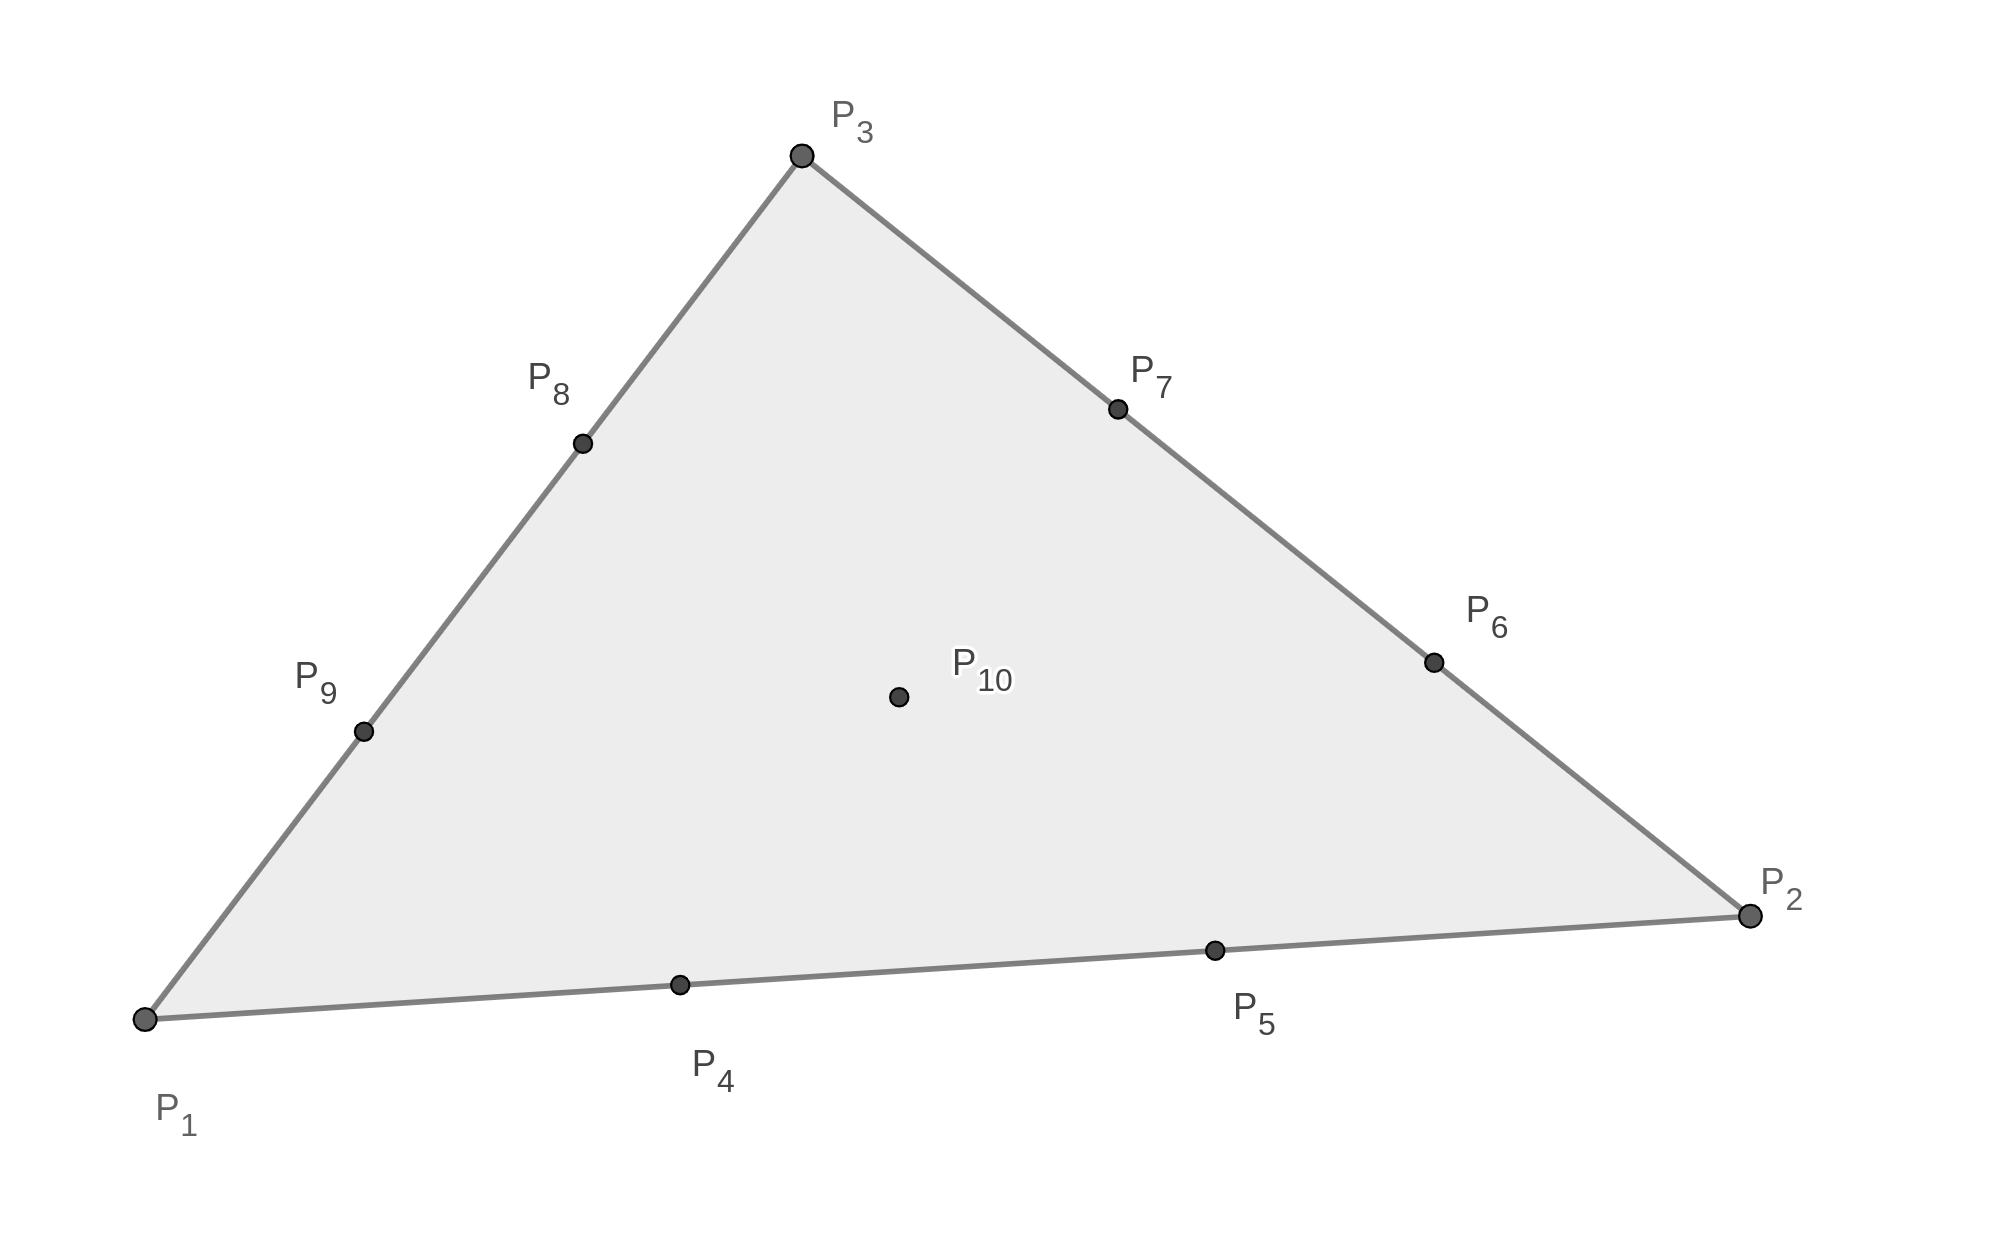
\includegraphics[width=0.4\textwidth]{images/cubic_on_triangular}
\captionsetup{labelformat=empty}
\caption{Նկար 2.9. Կետերի դասավորվածությունը կամայական եռանկյան վրա։}
\end{figure}

\end{enumerate}
Բնական է, որ որևէ կետի նկատմամբ լրիվ բազիսային ֆունկցիայի կառուցելու համար անհրաժեշտ է իրար գումարել այն բոլոր եռանկյուն էլեմենտների այդ կետին համապատասխան ֆունկցիաները, որոնց համար տվյալ կետը գագաթ է։
\newpage
\subsubsection*{2.2 Էրմիթյան ինտերպոլյացիա}
To be continued
\newpage
\section*{\centering Գլուխ 3 \\ Վարիացիոն մեթոդ}
\setcounter{equation}{0}
Վարիացիոն մեթոդները հանդիպում են բազմաթիվ ֆիզիկական խնդիրներում, և այդ խնդիրների մոտավոր լուծումը հիմնված է համապատասխան վարիացիոն մեթոդների վրա։
\subsection*{Սահմանումներ}
$f : \Omega \mapsto \Theta, \; \Omega \subset \mathbb{R}^{n}, \; \Theta \subset \mathbb{R}$ ֆունկցիայի $\epsilon$ շրջակայք ասելով կհասկանանք այն բոլոր $g$ ֆունկցիաների բազմությունը, որոնց համար տեղի ունի
\setcounter{equation}{0}
$$\left|f-g\right| < \epsilon$$պայմանը։
\subsection*{Խնդրի դրվածքը}
\hspace{\parindent}Վարիացիոն մեթոդի սկզբունքն այն է, որ դիտարկվող ֆունկցիայի ինտեգրալը տրված տիրույթում ընդունում է մեծագույն (փոքրագույն) արժեք տվյալ համակարգի իրական վիճակի համար, համեմատած բոլոր հնարավոր վիճակների բազմության հետ։  Ենթաինտեգրալային ֆունկցիան կախված է տրված կոորդինատներից, ֆունկցիայի արժեքից, նրա ածանցյալներից, իսկ ինտեգրումը կատարվում է տրված կոորդինատական համակարգում, որը կարող է ներառել նաև ժամանակը։ Մինիմումի որոշման խնդիրը հաճախ բերվում է մի քանի դիֆերենցիալ հավասարումների, համապատասխան եզրային պայմաններով։  Այն իրական փոփոխականի ֆունկցիայի էքստրեմումի որոնման խնդրի ընդհանրացումն է, որտեղ տրված ֆունկցիայի համար կոմպակտ տիրույթում անհրաժեշտ է գտնել այպիսի կետեր, որոնք մինիմում (մաքսիմում) են իրենց որևէ շրջակայքում։
Վարիացիոն մեթոդում ֆունկցիոնալը ինտեգրալ է, որը կախված է ֆուկցիայից, որի որոշման տիրույթը թույլատրելի ֆունկցիաների  տարածությունն է։
Այս  մեթոդի հիմնական դժվարությունը կայանում է նրանում, որ խնդիրները, որոնք կարող են ձևակերպվել որպես վարիացիոն, հնարավոր է, որ լուծում չունենան այն պատճառով, որ ֆունկցիոնալ տարածություները  կոմպակտ չեն։
Սակայն վարիացիոն մեթոդի հիմնական առավելությունն այն է, որ դրա կիրառման համար դրվող պահանջները ավելի թույլ են:
\newpage
\subsection*{Օրինակներ}
\hspace{\parindent}Որպես օրինակ դիտարկենք հետևյալ կրկնակի ինտեգրալը.
\begin{equation}
I\left(f\right)=\iint \limits_{\Omega} F\left(x, y, f, f_{x}, f_{y}\right)dxdy
\end{equation}
որտեղ $f \in C^{2}(\Omega)$,  $\Omega\subset \mathbb{R}^{2}$ և որի արժեքները որոշված են $\partial \Omega$ ում:
Այս դեպքում, որպեսզի $f$ ֆունկցիան $\left(1\right)$ ֆունկցիոնալի համարա հանդիսանա մինիմում, անհրաժեշտ է, որ $f(x,y)$ ֆունկցիան բավարարի Էյլեր֊Լագրանժի հավասարմանը, հավելելով համապատասխան եզրային պայմանները։
\begin{equation}
\dfrac{\partial}{\partial x}F_{u_{x}} + \dfrac{\partial}{\partial y}F_{u_{y}} - F_{u} = 0
\end{equation}
Օրինակ, $F = \dfrac{1}{2}\left(u_{x}^2+u_{y}^2\right)$ դեպքում խնդիրը բերվում է Լապլասի հավասարմանը.
\begin{equation}
\dfrac{\partial^{2}f}{\partial x^{2}} + \dfrac{\partial^{2}f}{\partial y^{2}} = 0
\end{equation}
Այժմ պարզ է, որ երկրորդ կարգի ածանցյալների անընդհատությունը անհրաժեշտ է Էյլեր֊Լագրանժի հավասարման գոյության համար։ Բայց վարիացիոն մեթոդը պահանջում է միայն $f$ ի անընդհատություն և առաջին կարգի մասնակի ածանցյալների կտոր առ կտոր անընդհատություն։
\subsection*{Ստացիոնար խնդիրներ}
Դիֆերենցիալ հավասարումը, որը կապված է վարիացիոն խնդրի հետ, կոչվում է Էյլեր֊Լագրանժի հավասարում։ Այս միայն անհրաժեշտ պայման է, որին պետք է բավարարի ֆունկցիան, որը մինիմիզացնում (մաքսիմիզացնում) է ֆունկցիոնալը։

\newpage
Ստորև դիտարկվում են խնդիրների մի քանի տարբերակներ.
\begin{enumerate}
\item Մեկ փոփոխականի ֆունկցիա.
$$f \in \Omega \mapsto \Theta, \; \Omega, \Theta \subset \mathbb{R}$$

\noindent Այս դեպքում ֆունկցիոնալն ընդունում է հետևյալ տեսքը.
$$I\left(f\right) = \int\limits_{x_0}^{x_{1}} F\left(x, f, f^{'}\right)dx$$

\noindent որտեղ $f(x_{0})$ և $f(x_{1})$, $x_{0}, x_{1} \in \Theta$ ը տրված են։
\noindent Մինիմիմում գոյության անհրաժեշտ պայման է հետևյալ դիֆերենցիալ հավասարումը.

$$\dfrac{\partial F}{\partial f} - \dfrac{d}{dx}\dfrac{\partial F}{\partial f^{'}}=0$$
Որը համարժեք է.
$$\dfrac{d^{2}f}{dx^{2}}F_{f^{'}f^{'}}+\dfrac{df}{dx}F_{f^{'}f} + F_{f^{'}x}-F_{f}=0$$

\item Մի քանի անհայտ ֆունկցիաներ.
$$f,g \in \Omega \mapsto \Theta, \; \Omega, \Theta \subset \mathbb{R}$$

\noindent Այս դեպքում ֆունկցիոնալն ընդունում է հետևյալ տեսքը.
$$I\left(f\right) = \int\limits_{x_0}^{x_{1}} F\left(x, f, g, f^{'}, g^{'}\right)dx$$

\noindent որտեղ $f(x_{0}), \; f(x_{1}), \; g(x_{0}), \; g(x_{1})$, $x_{0}, x_{1} \in \Theta$ ը տրված են։
\noindent Մինիմիմում գոյության անհրաժեշտ պայման է հետևյալ դիֆերենցիալ հավասարումների համակարգը.

$$\dfrac{\partial F}{\partial f} - \dfrac{d}{dx}\dfrac{\partial F}{\partial f^{'}}=0$$
$$\dfrac{\partial F}{\partial g} - \dfrac{d}{dx}\dfrac{\partial F}{\partial g^{'}}=0$$

\item Բարձր կարգի ածանցյալներ.
$$f \in \Omega \mapsto \Theta, \; \Omega, \Theta \subset \mathbb{R}$$

\noindent Այս դեպքում ֆունկցիոնալն ընդունում է հետևյալ տեսքը.
$$I\left(f\right) = \int\limits_{x_0}^{x_{1}} F\left(x, f, f^{'}, f^{''}, \dots, f^{(n)}\right)dx$$

\noindent որտեղ $f(x_{0}), \; f(x_{1}), \; f^{'}(x_{0}), \; f^{'}(x_{1})$, $x_{0}, x_{1} \in \Theta$ ը տրված են։
\noindent Մինիմիմում գոյության անհրաժեշտ պայման է հետևյալ դիֆերենցիալ հավասարումը.

$$\dfrac{\partial F}{\partial f} - \dfrac{d}{dx}\dfrac{\partial F}{\partial f^{'}} + \dfrac{d^{2}}{dx^{2}}\dfrac{\partial F}{\partial f^{''}} - \dots (-1)^{n}\dfrac{d^{n}}{dx^{n}}\dfrac{\partial F}{\partial f^{(n)}}=0$$

\item Մի քանի անկախ փոփոխականներ.
$$f \in \Omega \mapsto \Theta, \; \Omega \subset \mathbb{R}^{n}, \Theta \subset \mathbb{R}$$

\noindent Այս դեպքում ֆունկցիոնալն ընդունում է հետևյալ տեսքը.
$$I\left(f\right) = \idotsint \limits_{\Omega} F\left(x, f, f_{x_{1}}, f_{x_{2}}, \dots f_{x_{n} }\right)d\Omega$$
\noindent որտեղ $f$ ֆունկցիայի արժեքները $\partial \Omega$֊ի վրա տրված են։

\noindent Մինիմիմում գոյության անհրաժեշտ պայման է հետևյալ դիֆերենցիալ հավասարումը.

$$\dfrac{\partial F}{\partial f} - \dfrac{d}{dx_{1}}\dfrac{\partial F}{\partial f_{x_{1}}} - \dots -\dfrac{d}{dx_{n}}\dfrac{\partial F}{\partial f_{x_{n}}}=0$$
\end{enumerate}
\newpage
\subsubsection*{Եզրային պայմաններ}
Նախորդիվ դիտարկել էինք այնպիսի խնդիրներ, որտեղ ֆունկցիան արժեքները տրված տիրույթի եզրի տրված են։Սակայն որոշ խնդիրնորում ֆունկցիան տիրույթի եզրում տրված չէ, և տրվում են այլ տիպի եզրային պայմաններ։Նման դեպքերում որպես եզրային պայման դիտարկվում են հետևյալ պայմանները.

\noindent Մեկ փոփոխականի ֆունկցիա
$$\dfrac{\partial F}{\partial f^{'}}=0$$
Երկու անհայտ ֆունկցիա
$$\dfrac{\partial F}{\partial f^{'}}=\dfrac{\partial F}{\partial g^{'}}$$
Երկու փոփոխականի ֆունկցիա
$$F_{u_{x}}\dfrac{dy}{ds}-F_{u_{y}}\dfrac{dx}{ds}=0$$

\noindent որոնք հայտնի են որպես \emph{բնական կամ գլխավոր}  եզրային պայմաններ։

%TODO:  add continuation from Mitchel's book from 39 to 41 pages.
\subsubsection*{Պայմանական էքստրեմում}
Այսպիսի վարիացիոն խնդիրներում անհրաշետ է մինիմիզացնել (մաքսիմիզացնել) տրված ֆունկցիոնալը, պայմանով, որ մեկ այլ ֆունկցիոնալ ընդունում է որևէ ֆիքսված արժեք այդ ֆունկցիայի համար։ Այսինքն, եթե դիտարկենք ֆունկցիանալ, որի արժեքների բազմությունը մեկ փոփոխականի ֆունկցիաներ են, ապա կունենանք.

$$I\left(f\right)=\int \limits_{x_{0}}^{x_{1}} F\left(x, f, f^{'}\right)dx $$
$$\int \limits_{x_{0}}^{x_{1}} G\left(x, f, f^{'}\right)dx = C$$

Այս խնդրի համար Էյլեր֊Լագրանժի հավասարումը հետևյալն է.

$$\dfrac{\partial \left(F+\lambda G\right)}{\partial f} - \dfrac{d}{dx} \dfrac{\partial \left(F+\lambda G\right)}{\partial f^{'}} = 0$$


\newpage

%TODO: add description of finite elements

\section*{\centering Գլուխ 4 \\ Մոտավոր մեթոդներ։ Վերջավոր էլեմենտների մեթոդ}
\setcounter{equation}{0}
Խնդիրների վարիացիոն մեթոդով ձևակերպումը, և վարիացիոն մեթոդների ավելի թույլ պայմանները թույլ են տալիս այդ խնդիրները լուծել մոտավոր մեթոդներով, որոնք հաճախ անվանվում են ուղիղ մեթոդներ։ Ուղիղ մեթոդներից է Ռիտցի մինիմիզացնող հաջորդականության մեթոդը, որը քննության կառնենք։ 

\subsection*{Ռիտցի մեթոդ}
Դիտարկենք որևէ վարիացիոն մեթոդով տրված մինիմիզացիայի խնդիր.
		$$I\left(f\right) \longrightarrow min, \; f \in \Gamma$$
որտեղ $I$ ֆունկցիոնալը տրված տիրույթում որոշյալ ինտեգրալ է։
Մոտավոր լուծում կարելի է ստանալ, եթե ֆունկցիոնալի արժեքների բազմությունը սահմանափակենք որևէ վերջավոր չափանի ենթատարածությունով, որն ունի $\{\varphi_{j}\}_{j=1}^{N}$ բազիս։, 
			  $$\Gamma_{N} \in \Gamma $$
Ենթադրենք, որ $I$ ֆունկցիոնալի արժեքների տիրույթը ունի ճշգրիտ ստորին եզր, նշանակենք այն $\alpha_{0}$ ով։
Այդ դեպքում գոյություն ունի $\{f_{j}\}_{j=1}^{\infty}$ հաջորդականություն այնպիսին, որ
\begin{equation}
\lim_{n \to \infty}I\left(f_{n}\right) = \lim_{n \to \infty}I\left( \sum_{j=1}^{n} \gamma_{j}\varphi_{j} \right) = \alpha_{0}
\end{equation}
և ֆունկցիոնալի որոշման տիրույթի ցանկացած այլ $g$ ֆունկցիայի համար
			$$I\left(g\right) \geq \alpha_{0}$$
լուծումը փնտրենք հետևյալ կերպ.
\begin{equation}
f_{0}=\sum_{j=1}^{N}\gamma_{j}\varphi_{j}, \; \gamma_{j} \in \mathbb{R}
\end{equation}
Այդ դեպքում խնդիրը բերվում է սովորական մինիմումի խնդրի.
\begin{equation}
\dfrac{\partial I}{\partial \gamma_{i}} = \dfrac{\partial}{\partial \gamma_{i}} I \left(\sum_{j=1}^{N}\gamma_{j}\varphi_{j}\right) = 0
\end{equation}
\newpage
\subsection*{4.1 Պուասոնի հավասարման լուծում ուղղանկյուն տիրույթում}

Դիտարկենք հետևյալ դիֆերենցիալ հավասարումը.
\begin{equation}
\begin{cases}
			\Delta u =f \\
			u \Big |_{\partial D} = 0
\end{cases}
\end{equation}
որտեղ $D = \left[x_{0}, x_{N}\right] \times \left[y_{0}, y_{M}\right]$:

Այս դիֆերենցիալ հավասարման  համապատասխան վարիացիոն խնդիրը կլինի.
\begin{equation}
I(u) = \frac{1}{2}\iint \limits_{D} \left[u_x^2 + u_y^2 \right]dxdy + \iint \limits_{D} fudxdy \longrightarrow min
\end{equation}
D տիրույթը տրոհենք ուղղանկյուն եղանկյունների, և որպես բազիսային ֆունկցիաներ վերցնենք Կուրանտի ֆունկցիաները $\left(2.7\right)$։
Որոնելի ֆունկցիան կփնտրենք բազիսային ֆունկցիաների գծային կոմբինացիայի տեսքով.
\begin{equation}
u(x,y) = \sum_{i=0}^{N} \sum_{j=0}^{M} u_{ij}\varphi_{i, j}(x,y)
\end{equation}
Ուստի ինտեգրալային ֆունկցիոնալը կունենա հետևյալ տեսքը.
\begin{equation}
$$\scalemath{0.9}{\frac{1}{2} \iint \limits_{D}\left[\left(\sum_{i=0}^{N} \sum_{j=0}^{M}u_{ij}\varphi_{x}^{ij}(x,y)\right)^2 + \left(\sum_{i=0}^{N} \sum_{j=0}^{M}u_{ij}\varphi_{y}^{ij}(x,y)\right)^2 \right]dxdy + \iint \limits_{D}f(x,y)\left[ \sum_{i=0}^{N} \sum_{j=0}^{M}u_{ij}\varphi_{ij}(x,y)\right]dxdy}
\end{equation}
Համաձայն էքստրեմումի անհրաժեշտ պայմանի.
$$\dfrac{\partial I}{ \partial u_{kl}} = \dfrac{\partial}{\partial u_{kl}} I \left(\sum_{j=0}^{M} u_{ij}\varphi_{i, j}(x,y)\right) = 0 $$

Դիտարկենք առաջին կրկնակի գումարը.

				$$\left(\sum_{i=0}^{N} \sum_{j=0}^{M}u_{ij}\varphi_{x}^{ij}(x,y)\right)^2 = \left[u_{kl}\varphi_{x}^{kl}(x,y)\right]^{2} + 2u_{kl}\varphi_{x}^{kl}(x,y)[\dots] + [\dots]^2$$
որտեղ բազմակետերով արտահայտությունը իր մեջ չի պարունակում $u_{kl}$ ը։
Հանգունորեն, երկրորդ կրկնակի գումարի համար՝
				$$\left(\sum_{i=0}^{N} \sum_{j=0}^{M}u_{ij}\varphi_{y}^{ij}(x,y)\right)^2 = \left[u_{kl}\varphi_{y}^{kl}(x,y)\right]^{2} + 2u_{kl}\varphi_{y}^{kl}(x,y)[\dots] + [\dots]^2$$

Այսպիսով ավելի պարզեցված տեսքով համակարգը ունի հետևյալ տեսքը.
$$\scalemath{0.85}{\frac{\partial}{\partial u_{kl}}I \left(u\right)= \iint \limits_{D} \left[2u_{kl}\left\{\varphi_{x}^{kl}(x,y)\right\}^{2} + 2\varphi_{x}^{kl}(x,y)[\dots] + 2u_{kl}\left\{\varphi_{y}^{kl}(x,y)\right\}^{2} + 2\varphi_{y}^{kl}(x,y)[\dots] + 2f(x,y)\varphi^{kl}(x,y)\right]dxdy}$$
Դիտարկենք $\varphi_{x}^{kl}(x,y) $ և $\varphi_{y}^{kl}(x,y) $ ֆունկցիաները։
\begin{equation}
\varphi_{x}^{kl}(x,y)  = \begin{cases}
\phantom{-}0, &(x,y) \in S_{1} \\
\phantom{-}\dfrac{1}{h_{1}}, &(x,y) \in S_{2} \\
\phantom{-}\dfrac{1}{h_{1}}, &(x,y) \in S_{3} \\
\phantom{-}0, &(x,y) \in S_{4} \\
-\dfrac{1}{h_{1}}, &(x,y) \in S_{5} \\
-\dfrac{1}{h_{1}}, &(x,y) \in S_{6}\\
0, \text{մնացած դեպքերում}
\end{cases}
\end{equation}
\begin{equation}
\varphi_{y}^{kl}(x,y)  = \begin{cases}
-\dfrac{1}{h_{2}}, &(x,y) \in S_{1} \\
-\dfrac{1}{h_{2}}, &(x,y) \in S_{2} \\
\phantom{-}0, &(x,y) \in S_{3} \\
\phantom{-}\dfrac{1}{h_{2}}, &(x,y) \in S_{4} \\
\phantom{-}\dfrac{1}{h_{2}}, &(x,y) \in S_{5} \\
0, &(x,y) \in S_{6}\\
0, \text{մնացած դեպքերում}
\end{cases} \;
\end{equation}

Քանի որ $\varphi_{x}^{kl}(x,y) $ և $\varphi_{y}^{kl}(x,y) $ ֆունկցիաները ոչ զրոյական են $\left[x_{k-1, l}, x_{k+1, l} \right] \times \left[y_{k, l-1}, y_{k, l+1}\right]$ ում, ապա

\begin{equation}
\iint \limits_{D} 2u_{kl}\left\{\varphi_{x}^{kl}(x,y)\right\}^{2}dxdy = 4u_{kl}\dfrac{h_{2}}{h_{1}}
\end{equation}
\begin{equation}
\iint \limits_{D} 2u_{kl}\left\{\varphi_{y}^{kl}(x,y)\right\}^{2}dxdy = 4u_{kl}\dfrac{h_{1}}{h_{2}}
\end{equation}
Քանի որ յուրաքանչյուր $\varphi_{kl}$ բազիսային ֆունկցիա հատվում Է $\varphi_{k-1, l}$, $\varphi_{k+1, l}$, $\varphi_{k, l-1}$, $\varphi_{k, l+1}$ ֆունկցիաների հետ, ապա
\begin{equation}
\begin{gathered}
\iint \limits_{D} 2\varphi_{x}^{kl}(x,y)[\dots]dxdy = \cr
=\scalemath{0.85}{2\iint \limits_{D} \varphi_{x}^{kl}(x,y)[u_{k-1,l}\varphi_{x}^{k-1, l}(x,y)+u_{k+1,l}\varphi_{x}^{k+1, l}(x,y)+u_{k,l-1}\varphi_{x}^{k, l-1}(x,y)+u_{k,l+1}\varphi_{x}^{k, l+1}(x,y)]dxdy =} \cr
= -2u_{k-1, l}\dfrac{h_{2} }{h_{1}} -2u_{k+1, l}\dfrac{ h_{2}}{h_{1}}
\end{gathered}
\end{equation}
Հանգունորեն՝
\begin{equation}
\scalemath{0.85}{2 \iint \limits_{D}\varphi_{y}^{kl}(x,y)[\dots]dxdy =  -2u_{k, l-1}\dfrac{h_{1}} {h_{2}} - 2u_{k, l+1}\dfrac{h_{1}}{ h_{2}}}$$
\end{equation}
Եվ վերջապես
\begin{equation}
2\iint \limits_{D} f(x,y)\varphi_{kl}(x,y)dxdy \approx 2 f_{kl} h_{1} h_{2}
\end{equation}
Դիրիխլեի եզրային պայմանների համար կունենանք։
$$u_{0, l} = u_{N, l} = u_{k, 0} = u_{k, M} = 0$$
Այսպիսով, ստացանք հետևյալ հավասարումների համակարգը.
\begin{equation}
\begin{cases}
			2\left[\dfrac{1}{h^{2}_{1}} + \dfrac{1}{h^{2}_{2}}\right] u_{kl}  -\dfrac{1}{h^{2}_{1}}u_{k-1, l} - \dfrac{1}{h^{2}_{1}}u_{k+1, l} -\dfrac{1}{h^{2}_{2}}u_{k, l-1} - \dfrac{1}{h^{2}_{2}}u_{k, l+1} + f_{kl} = 0\\
			u_{0, l} = u_{N, l} = u_{k, 0} = u_{k, M} = 0
\end{cases}
\end{equation}
\newpage
\subsubsection*{Ծրագրային իրականացում}

Պուասոնի հավասարման մոտավուր լուծումը իրականացնելու համար օգտվենք Python ծրագրավորմալ լեզվից, օգտագործելով Numpy գրադարանը, որը հարմար է բազմաչափ զանգվածների հետ մաթեմատիկական գործողություններ իրականացնալու համար։ Վիզուալիզացիաները կառուցելու համար կօգտվենք Matplotlib գրադարանից։

Ծրագրի սկզբում տրվում է ուղղանկյուն տիրույթի սահմանները և դրա տրոհման $h_{1}$ և $h_{2}$ քայլերը, $f$ ֆունկցիան։ Հաջորդիվ կազմվում է հավասարումների համակարգը, կանչվում այն լուծող ֆունկցիան։ Այսնուհետև բազիսային ֆունկցիաների միջոցով կառուցվում է մոտարկող ֆունկցիան։

Օրինակ


				$$
					\begin{cases}
								\Delta u =2 \\
								u \Big |_{\partial D} = 0
					\end{cases}
				$$

				$$ D = \left[-\dfrac{\pi}{2}, \phantom{-}\dfrac{\pi}{2}\right] \times \left[-\dfrac{\pi}{2}, \phantom{-}\dfrac{\pi}{2}\right], \; h_{1}=h_{2}=\dfrac{\pi}{200}$$
Խնդրի համար ստացված լուծումը.
\begin{figure}[H]
\centering
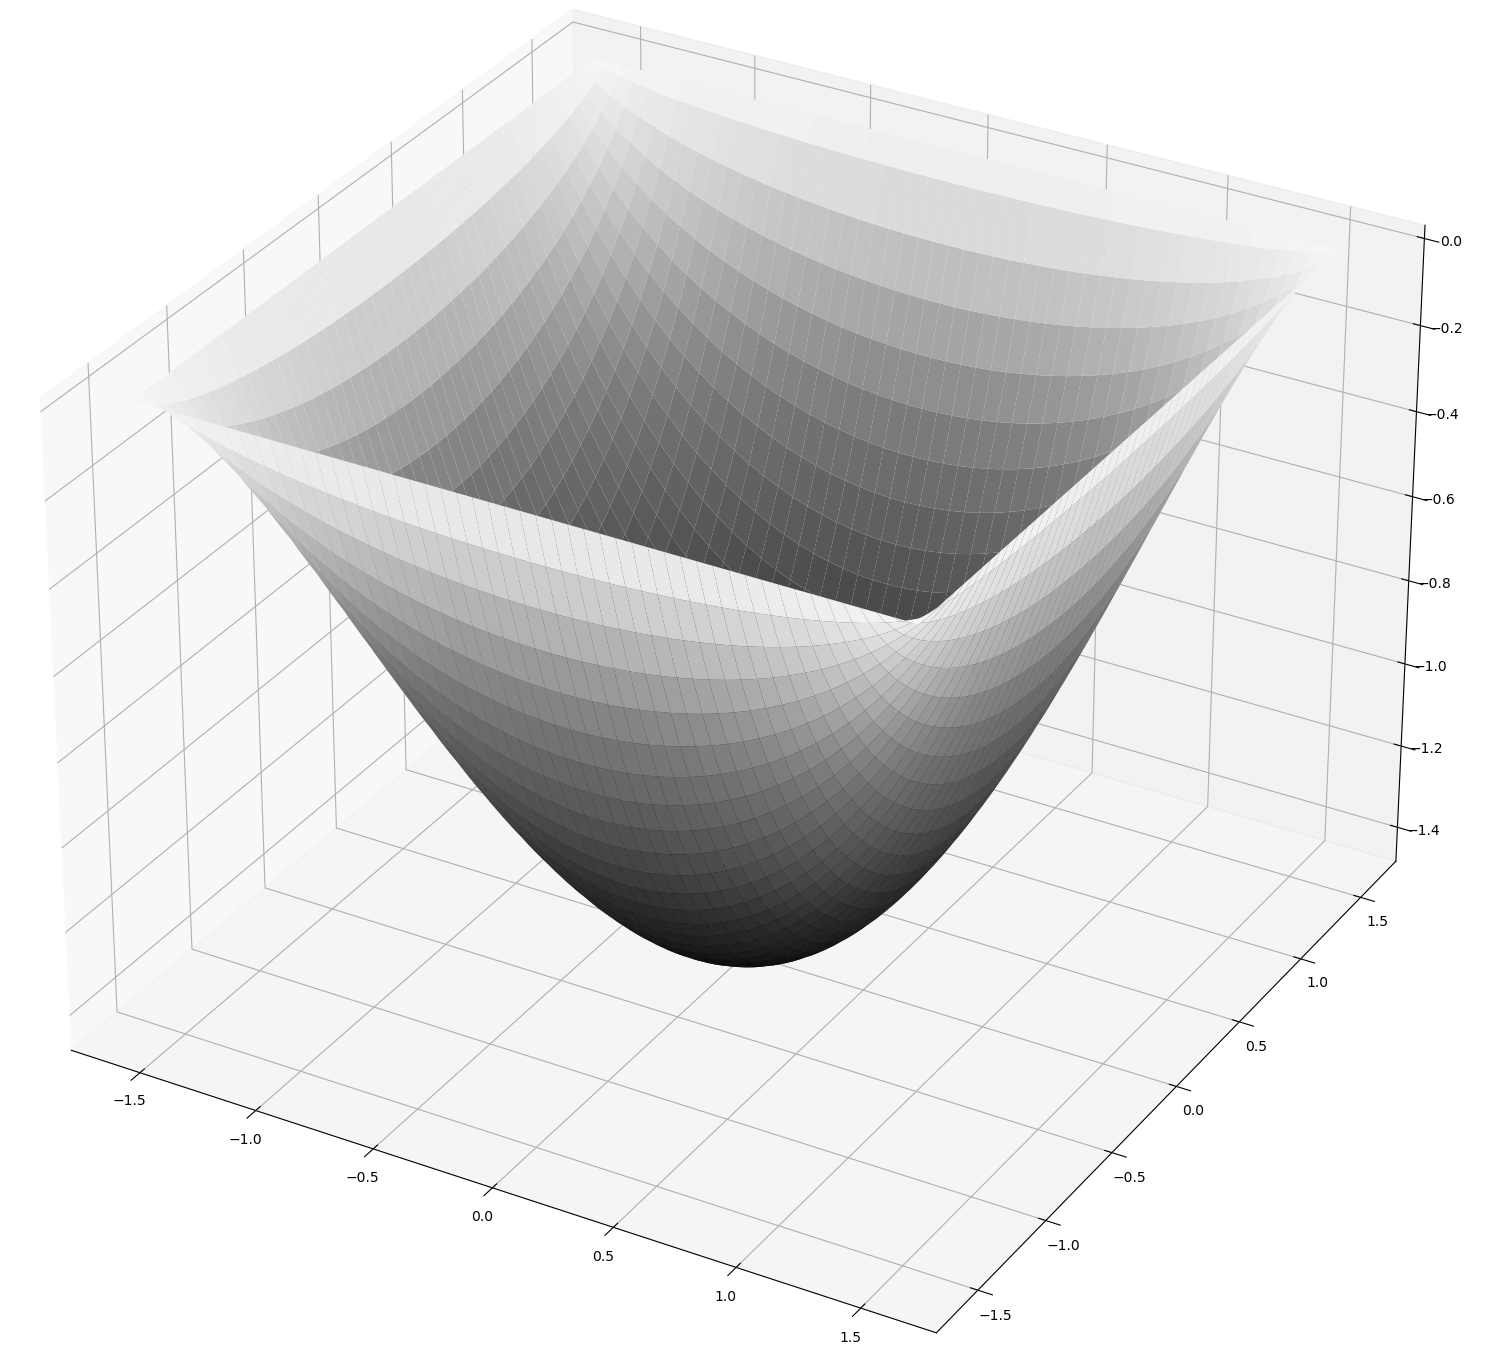
\includegraphics[width=0.7\textwidth]{images/poisson_solution}
\captionsetup{labelformat=empty}
\caption{Նկար 4.1. Պուասոնի հավասարման լուծման գրաֆիկական ներկայացում։}
\end{figure}
\newpage
\subsection*{4.2 Պուասոնի հավասարման լուծում եռանկյունացվող}

Դիտարկենք հետևյալ դիֆերենցիալ հավասարումը.
\begin{equation}
\begin{cases}
			\Delta u =f \\
			u \Big |_{\partial D} = 0
\end{cases}
\end{equation}
որտեղ $D$֊ն կամայական տիրույթ է։

Այս դիֆերենցիալ հավասարման  համապատասխան վարիացիոն խնդիրը կլինի.
\begin{equation}
I(u) = \frac{1}{2}\iint \limits_{D} \left[u_x^2 + u_y^2 \right]dxdy + \iint \limits_{D} fudxdy \longrightarrow min
\end{equation}

D տիրույթը տրոհենք $N$ եռանկյունների։ Գագաթների համարակալումը կկատարենք հետևյալ կերպ. յուրաքանչյուր եռանկյան ներսում գագաթները կհամարակալենք $1, 2, 3$ թվերով ժամսլաքին հակառակ ուղղությամբ, որին կանվանենք լոկալ համարակալում, միևնույն ժամանակ գագաթները համարակալելով ամբողջ տիրույթի համար, որին կանվանենք գլոբալ համարակալում։ 
\begin{figure}[H]
\centering
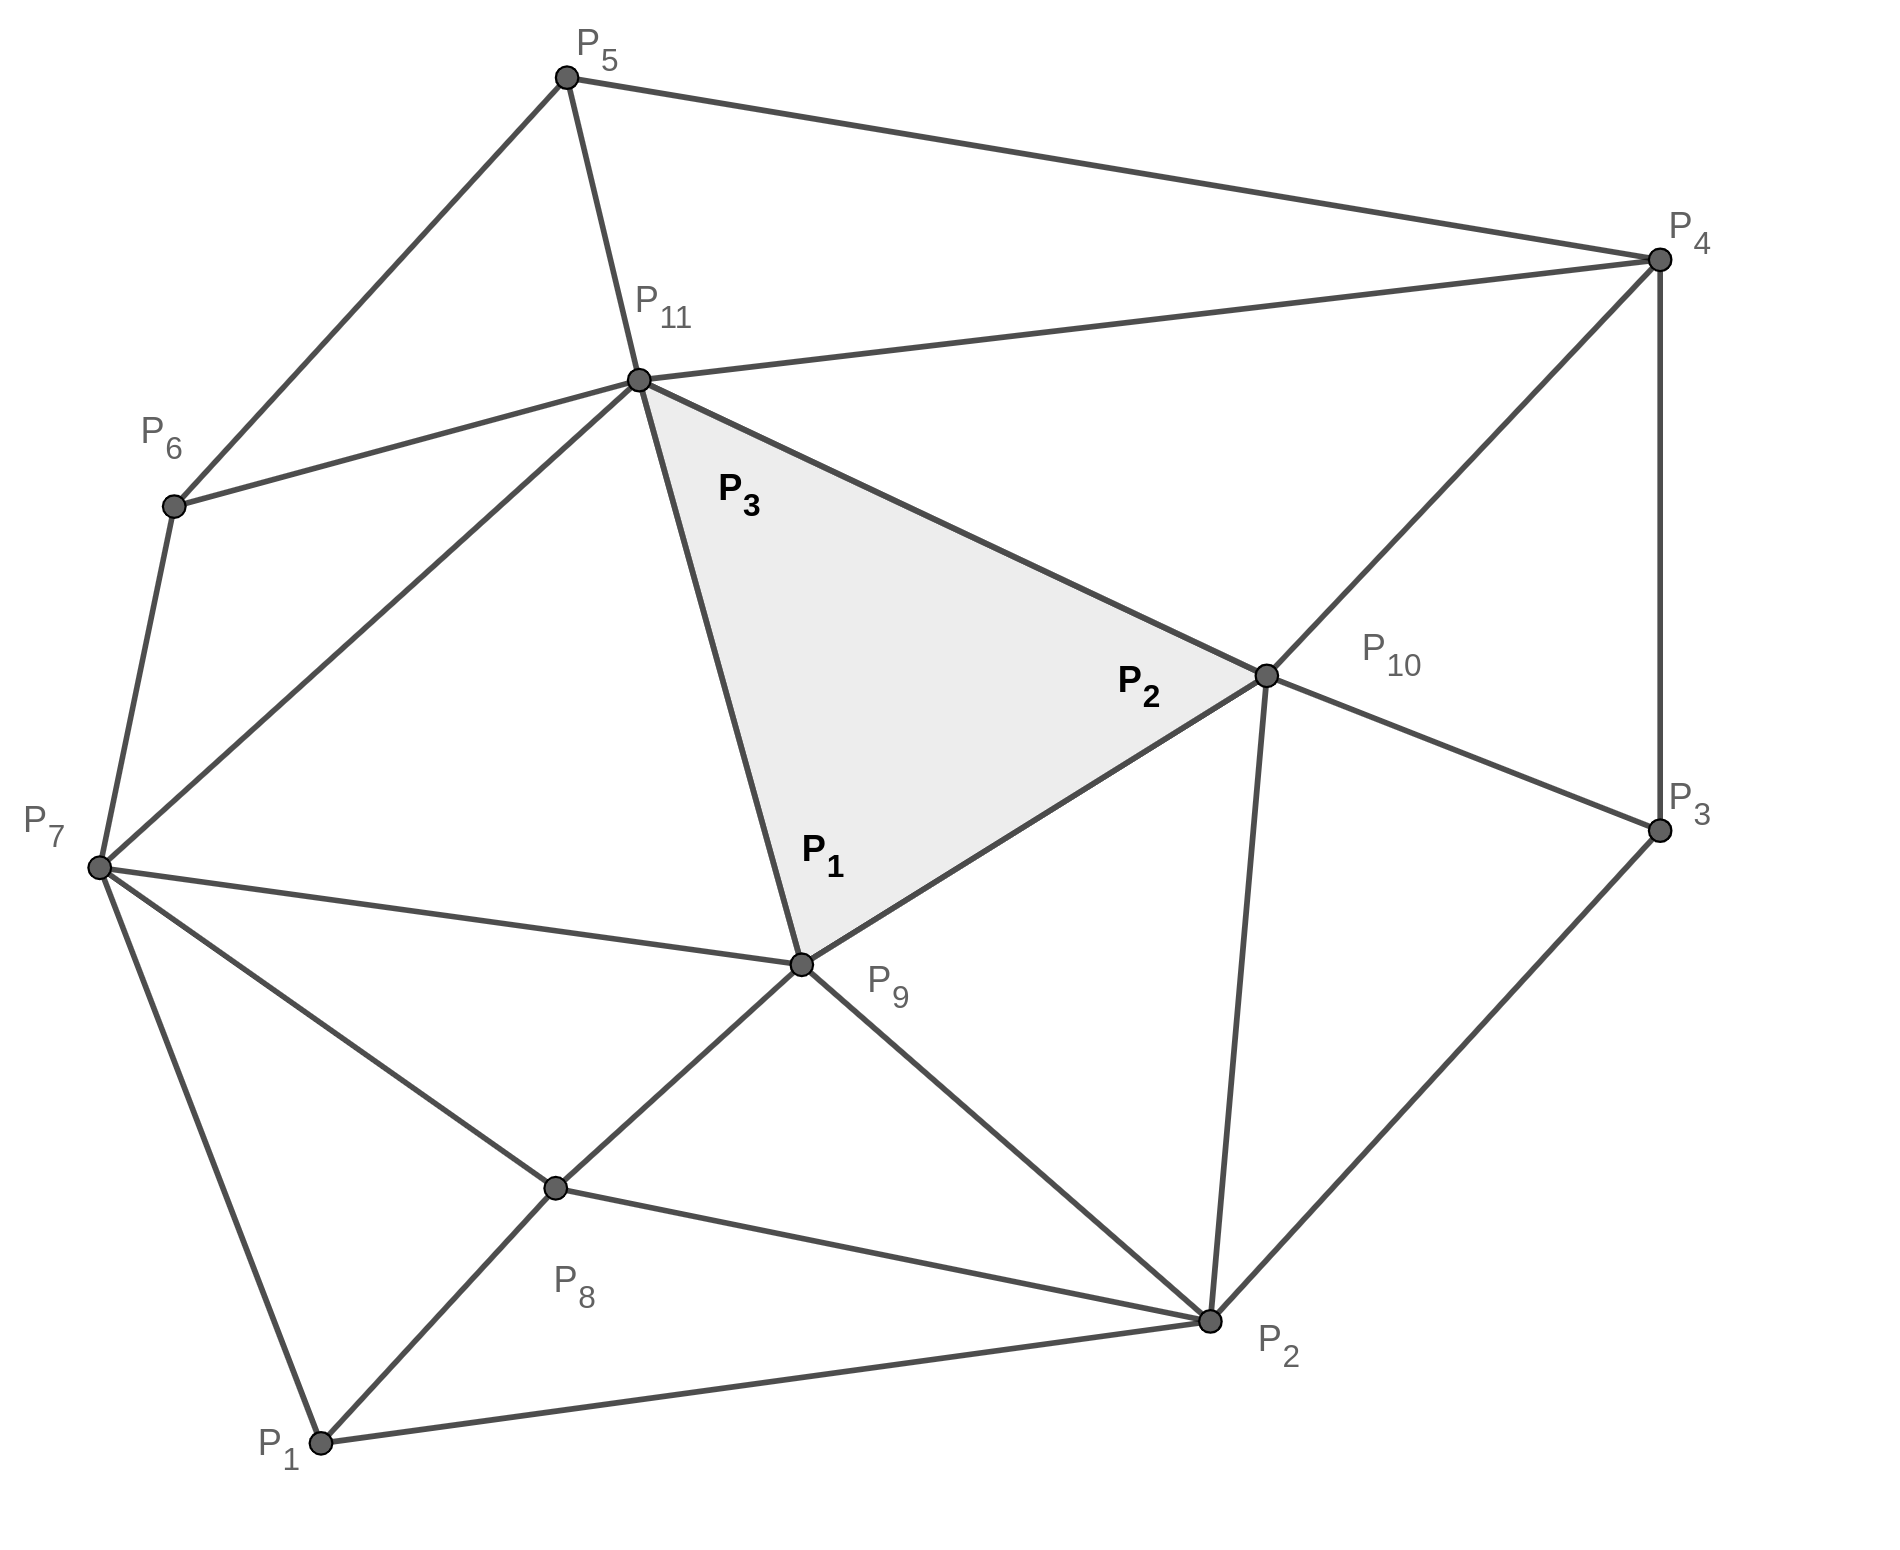
\includegraphics[width=0.7\textwidth]{images/global_and_local_numbering}
\captionsetup{labelformat=empty}
\caption{Նկար 4.2. Գագաթների լոկալ (թավ տառատեսակ) և գլոբալ համարակալման օրինակ։}
\end{figure}
Յուրաքանչյուր $\Delta_{n}$ եռանկյան վրա ($n=\overline{1, N}$) որպես բազիսային ֆունկցիաներ վերցնենք $\left(2.13\right)$֊ում ներկայացված ֆունկցիաները, և որոնելի ֆունկցիան կփնտրենք բազիսային ֆունկցիաների գծային կոմբինացիայի տեսքով.
\begin{equation}
u(x, y) = \dfrac{1}{S_{n}}\sum_{i=1}^{3}u_{ni}p^{(ni)}(x,y)
\end{equation}
որտեղ $ni$֊ն $n$֊րդ եռանկյան $i$֊րդ գագաթի համապատասխան ինդեքսն է, իսկ $p^{(ni)}(x,y)$֊ն այդ գագաթի համապատասխան բազիսային ֆունկցիան է։
Ուստի ինտեգրալային ֆունկցիոնալը կունենա հետևյալ տեսքը.
\begin{equation}
$$\scalemath{0.9}{\frac{1}{2S_{n}^{2}} \iint \limits_{\Delta_{n}}\left[\left(\sum_{i=1}^{3}u_{ni}p^{(ni)}_{x}(x,y)\right)^2 + \left(\sum_{i=1}^{3}u_{ni}p^{(ni)}_{y}(x,y)\right)^2 \right]dxdy + \dfrac{1}{S_{n}}\iint \limits_{D}f(x,y)\left[ \sum_{i=1}^{3}u_{ni}p^{(ni)}(x,y)\right]dxdy}
\end{equation}
Համաձայն էքստրեմումի անհրաժեշտ պայմանի.
\begin{equation}
\dfrac{\partial I}{ \partial u_{nk}} = \dfrac{\partial}{\partial u_{nk}} I \left(\dfrac{1}{S_{n}}\sum_{i=1}^{3}u_{ni}p^{(i)}(x,y)\right) = 0
\end{equation}
Դիտարկենք $\left(4.18\right)$ ինտեգրալի ենթաինտեգրալային արտահայտության ձախ մասի երկու մասերը.

\begin{equation}
\begin{aligned}
&\left(\sum_{i=1}^{3}u_{ni}p^{(ni)}_{x}(x,y)\right)^2=\left(u_{nk}p_{x}^{(nk)}\right)^{2}+2u_{nk}u_{nl}p_{x}^{(nk)}p_{x}^{(nl)}+2u_{nk}u_{nm}p_{x}^{(nk)}p_{x}^{(nm)} \\
&\left(\sum_{i=1}^{3}u_{ni}p^{(ni)}_{y}(x,y)\right)^2=\left(u_{nk}p_{y}^{(nk)}\right)^{2}+2u_{nk}u_{nl}p_{y}^{(nk)}p_{y}^{(nl)}+2u_{nk}u_{nm}p_{y}^{(nk)}p_{y}^{(nm)} \\
\end{aligned}
\end{equation}

\noindent որտեղ $k, l, m$֊ը գագաթների հաջորդականությունն է լոկալ համարակալման մեջ։

Այսպիսով ավելի պարզեցված տեսքով համակարգը ունի հետևյալ տեսքը.
\begin{equation}
\scalemath{0.70}{\frac{\partial}{\partial u_{nk}}I \left(u\right)= \iint \limits_{\Delta_{n}} \left[u_{nk}\left(p_{x}^{(nk)}\right)^{2}+u_{nl}p_{x}^{(nk)}p_{x}^{(nl)}+u_{nm}p_{x}^{(nk)}p_{x}^{(nm)}+u_{nk}\left(p_{y}^{(nk)}\right)^{2}+u_{nl}p_{y}^{(nk)}p_{y}^{(nl)}+u_{nm}p_{y}^{(nk)}p_{y}^{(nm)} + S_{n}u_{nk}p^{(nk)}\right]dxdy=0}
\end{equation}
Քանի որ
$$p_{x}^{(nk)} = \left(y_{nl}-y_{nm}\right)$$
$$p_{y}^{(nk)} = -\left(x_{nl}-x_{nm}\right)$$
ապա
\begin{equation}
\begin{aligned}
&\iint \limits_{\Delta_{n}}2u_{nk}\left(p_{x}^{(nk)}\right)^{2}dxdy = 2u_n{k} S_{n} \left(y_{nl}-y_{nm}\right)^{2} \\
&\iint \limits_{\Delta_{n}}2u_{nl}p_{x}^{(nk)}p_{x}^{(l)}dxdy = 2u_{nl} S_{n} \left(y_{nl}-y_{nm}\right)\left(y_{nm}-y_{nk}\right) \\
&\iint \limits_{\Delta_{n}}2u_{nm}p_{x}^{(nk)}p_{x}^{(nm)}dxdy = 2u_{nm} S_{n} \left(y_{nl}-y_{nm}\right)\left(y_{nk}-y_{nl}\right) \\
&\iint \limits_{\Delta_{n}}2u_{nk}\left(p_{y}^{(nk)}\right)^{2}dxdy = 2u_{nk} S_{n} \left(x_{nl}-x_{nm}\right)^{2} \\
&\iint \limits_{\Delta_{n}}2u_{nl}p_{y}^{(nk)}p_{y}^{(nl)}dxdy = 2u_{nl} S_{n} \left(x_{nl}-x_{nm}\right)\left(x_{nm}-x_{nk}\right) \\
&\iint \limits_{\Delta_{n}}2u_{nm}p_{y}^{(nk)}p_{y}^{(nm)}dxdy = 2u_{nm} S_{n} \left(x_{nl}-x_{nm}\right)\left(x_{nk}-x_{nl}\right) \\
&\iint \limits_{\Delta_{n}}2S_{n}p^{(nk)}dxdy \approx \dfrac{2}{3}u_{nk} S_{n}^{2}f_{nk} \\
\end{aligned}
\end{equation}
Նշանակենք
$$\begin{aligned}
y_{ni}-y_{nj} = y_{nij} \\
x_{ni}-y_{nj} = x_{nij} \\
\end{aligned}$$
Այսպիսով, $\Delta_{n}$ եռանկյան համար ստացանք հետևյալ հավասարումների համակարգը.
\begin{equation}
\scalemath{0.9}
{
\begin{cases}
2u_{nk}S_{n}\left(y_{nlm}^{2}+x_{nlm}^{2}\right)+2u_{nl}S_{n}\left(y_{nlm}y_{nmk}+x_{nlm}x_{nmk}\right)+2u_{m}S_{n}\left(y_{nlm}y_{nkl}+x_{nlm}x_{nkl}\right)=-\dfrac{2}{3}u_{nk} S_{n}^{2}f_{nk} \\
u_{nk} = 0, \text{եթե } u_{nk}\text{֊ն տիրույթի եզրի գագաթ է}
\end{cases}
}
\end{equation}
Համախմբելով բոլոր եռանկյունների համար ստացված հավասարումները, կստանանք գլխավոր համակարգը, և յուրաքանչյուր $n$֊րդ գագաթի համար կունենանք.
\begin{equation}
\scalemath{0.8}
{
\begin{cases}
\sum_{r: P_{n} \in \Delta{r}}u_{nk}S_{r}\left(y_{rlm}^{2}+x_{rlm}^{2}\right)+u_{nl}S_{r}\left(y_{rlm}y_{rmk}+x_{rlm}x_{rmk}\right)+u_{m}S_{r}\left(y_{rlm}y_{rkl}+x_{rlm}x_{rkl}\right)=-\dfrac{1}{3}\sum_{r: P_{n} \in \Delta{r}}u_{nk} S_{r}^{2}f_{nk} \\
u_{nk} = 0, \text{եթե } u_{nk}\text{֊ն տիրույթի եզրի գագաթ է}
\end{cases}
}
\end{equation}

\begin{figure}[H]
\centering
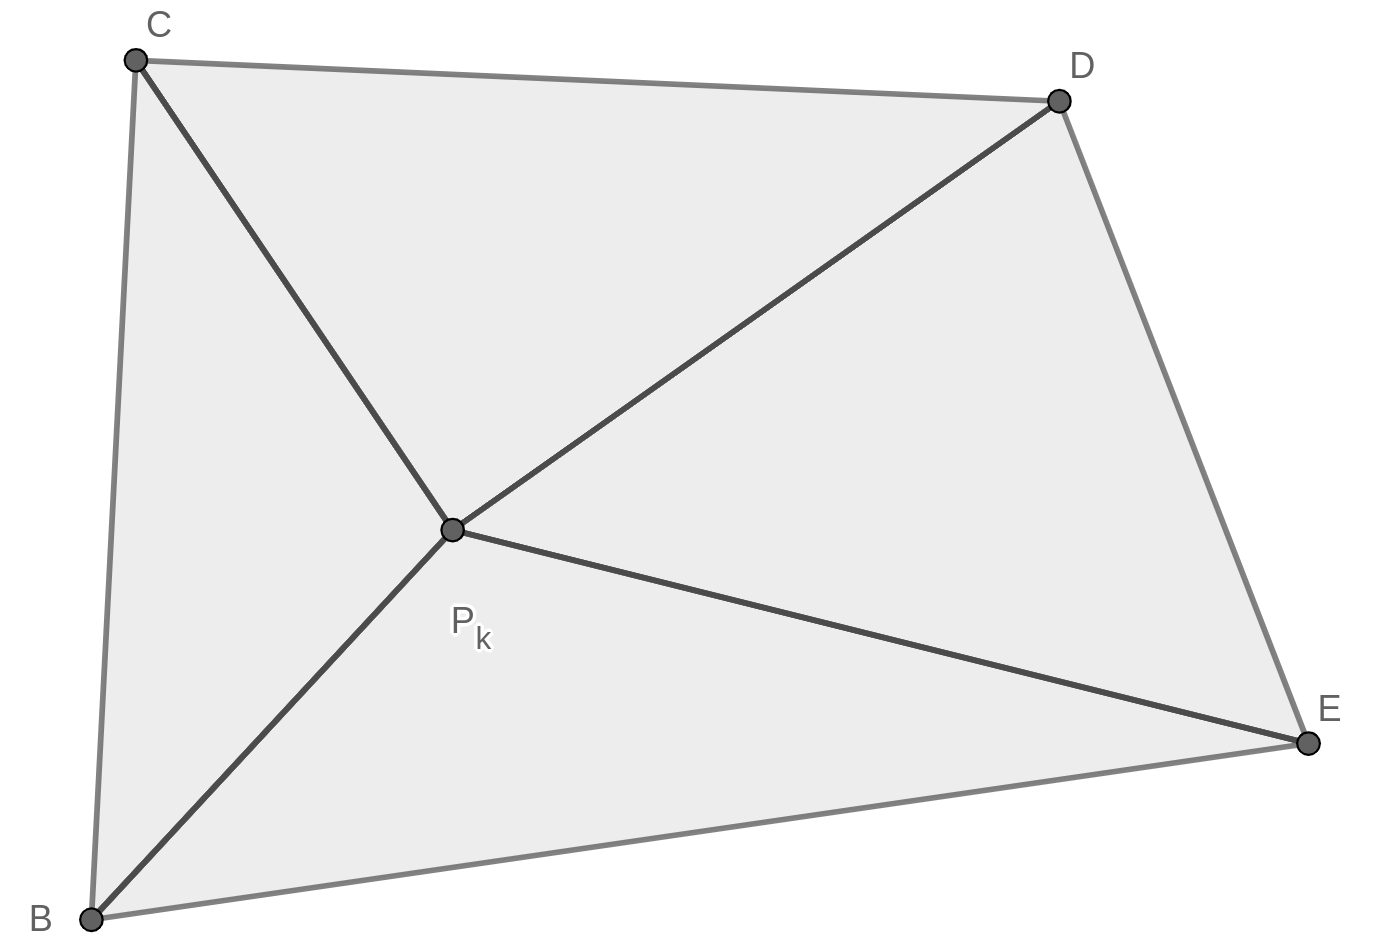
\includegraphics[width=0.7\textwidth]{images/assembling_equation}
\captionsetup{labelformat=empty}
\caption{Նկար 4.3. Գլխավոր համակարգի համախմբում։}
\end{figure}
\newpage
\subsubsection*{Ծրագրային իրականացում}

Ինչպես ուղղանկյուն տիրույթի դեպքում, այնպես էլ այս դեպքում կօգտվենք նույն գործիքներից։ Տիրույթի եռանկյունացման համար կօգտվենք $Python$ ծրագրավորման լեզվի triangle գրադարանից.

Ծրագրի սկզբում տրվում է տիրույթի եզրագծի կետերը, եզրագծերի կետերի միացման հաջորդականությունը, եռանկյունացման պարամետրերը և $f$ ֆունկցիան։ Հաջորդիվ յուրաքանչյուր եռանկյան համար կազմվում է հավասարումների համակարգը, հընթացս կառուցելով գլխավոր հավասարումների համակարգը։ Այնուհետև կանչվում այն լուծող ֆունկցիան։ Այնուհետև բազիսային ֆունկցիաների միջոցով կառուցվում է մոտարկող ֆունկցիան։

Օրինակ

$$
  \begin{cases}
        \Delta u =2 \\
        u \Big |_{\partial D} = 0
  \end{cases}
$$

$$ D = \left\{\left(x,y\right): x^{2}+y^{2} \leq 1\right\}$$
Տիրույթի եռանկյունացումը
\begin{figure}[H]
\centering
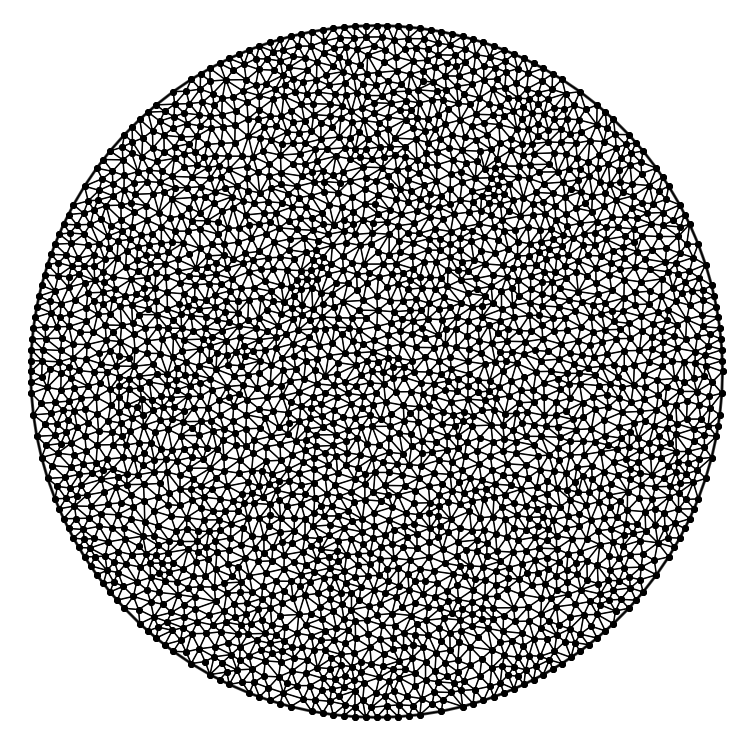
\includegraphics[width=0.6\textwidth]{images/circle_mesh}
\captionsetup{labelformat=empty}
\caption{Նկար 4.4. Շրջանաձև տիրույթի եռանկյունացման երկրաչափական ներկայացում։}
\end{figure}
Խնդրի համար ստացված լուծումը.
\begin{figure}[H]
\centering
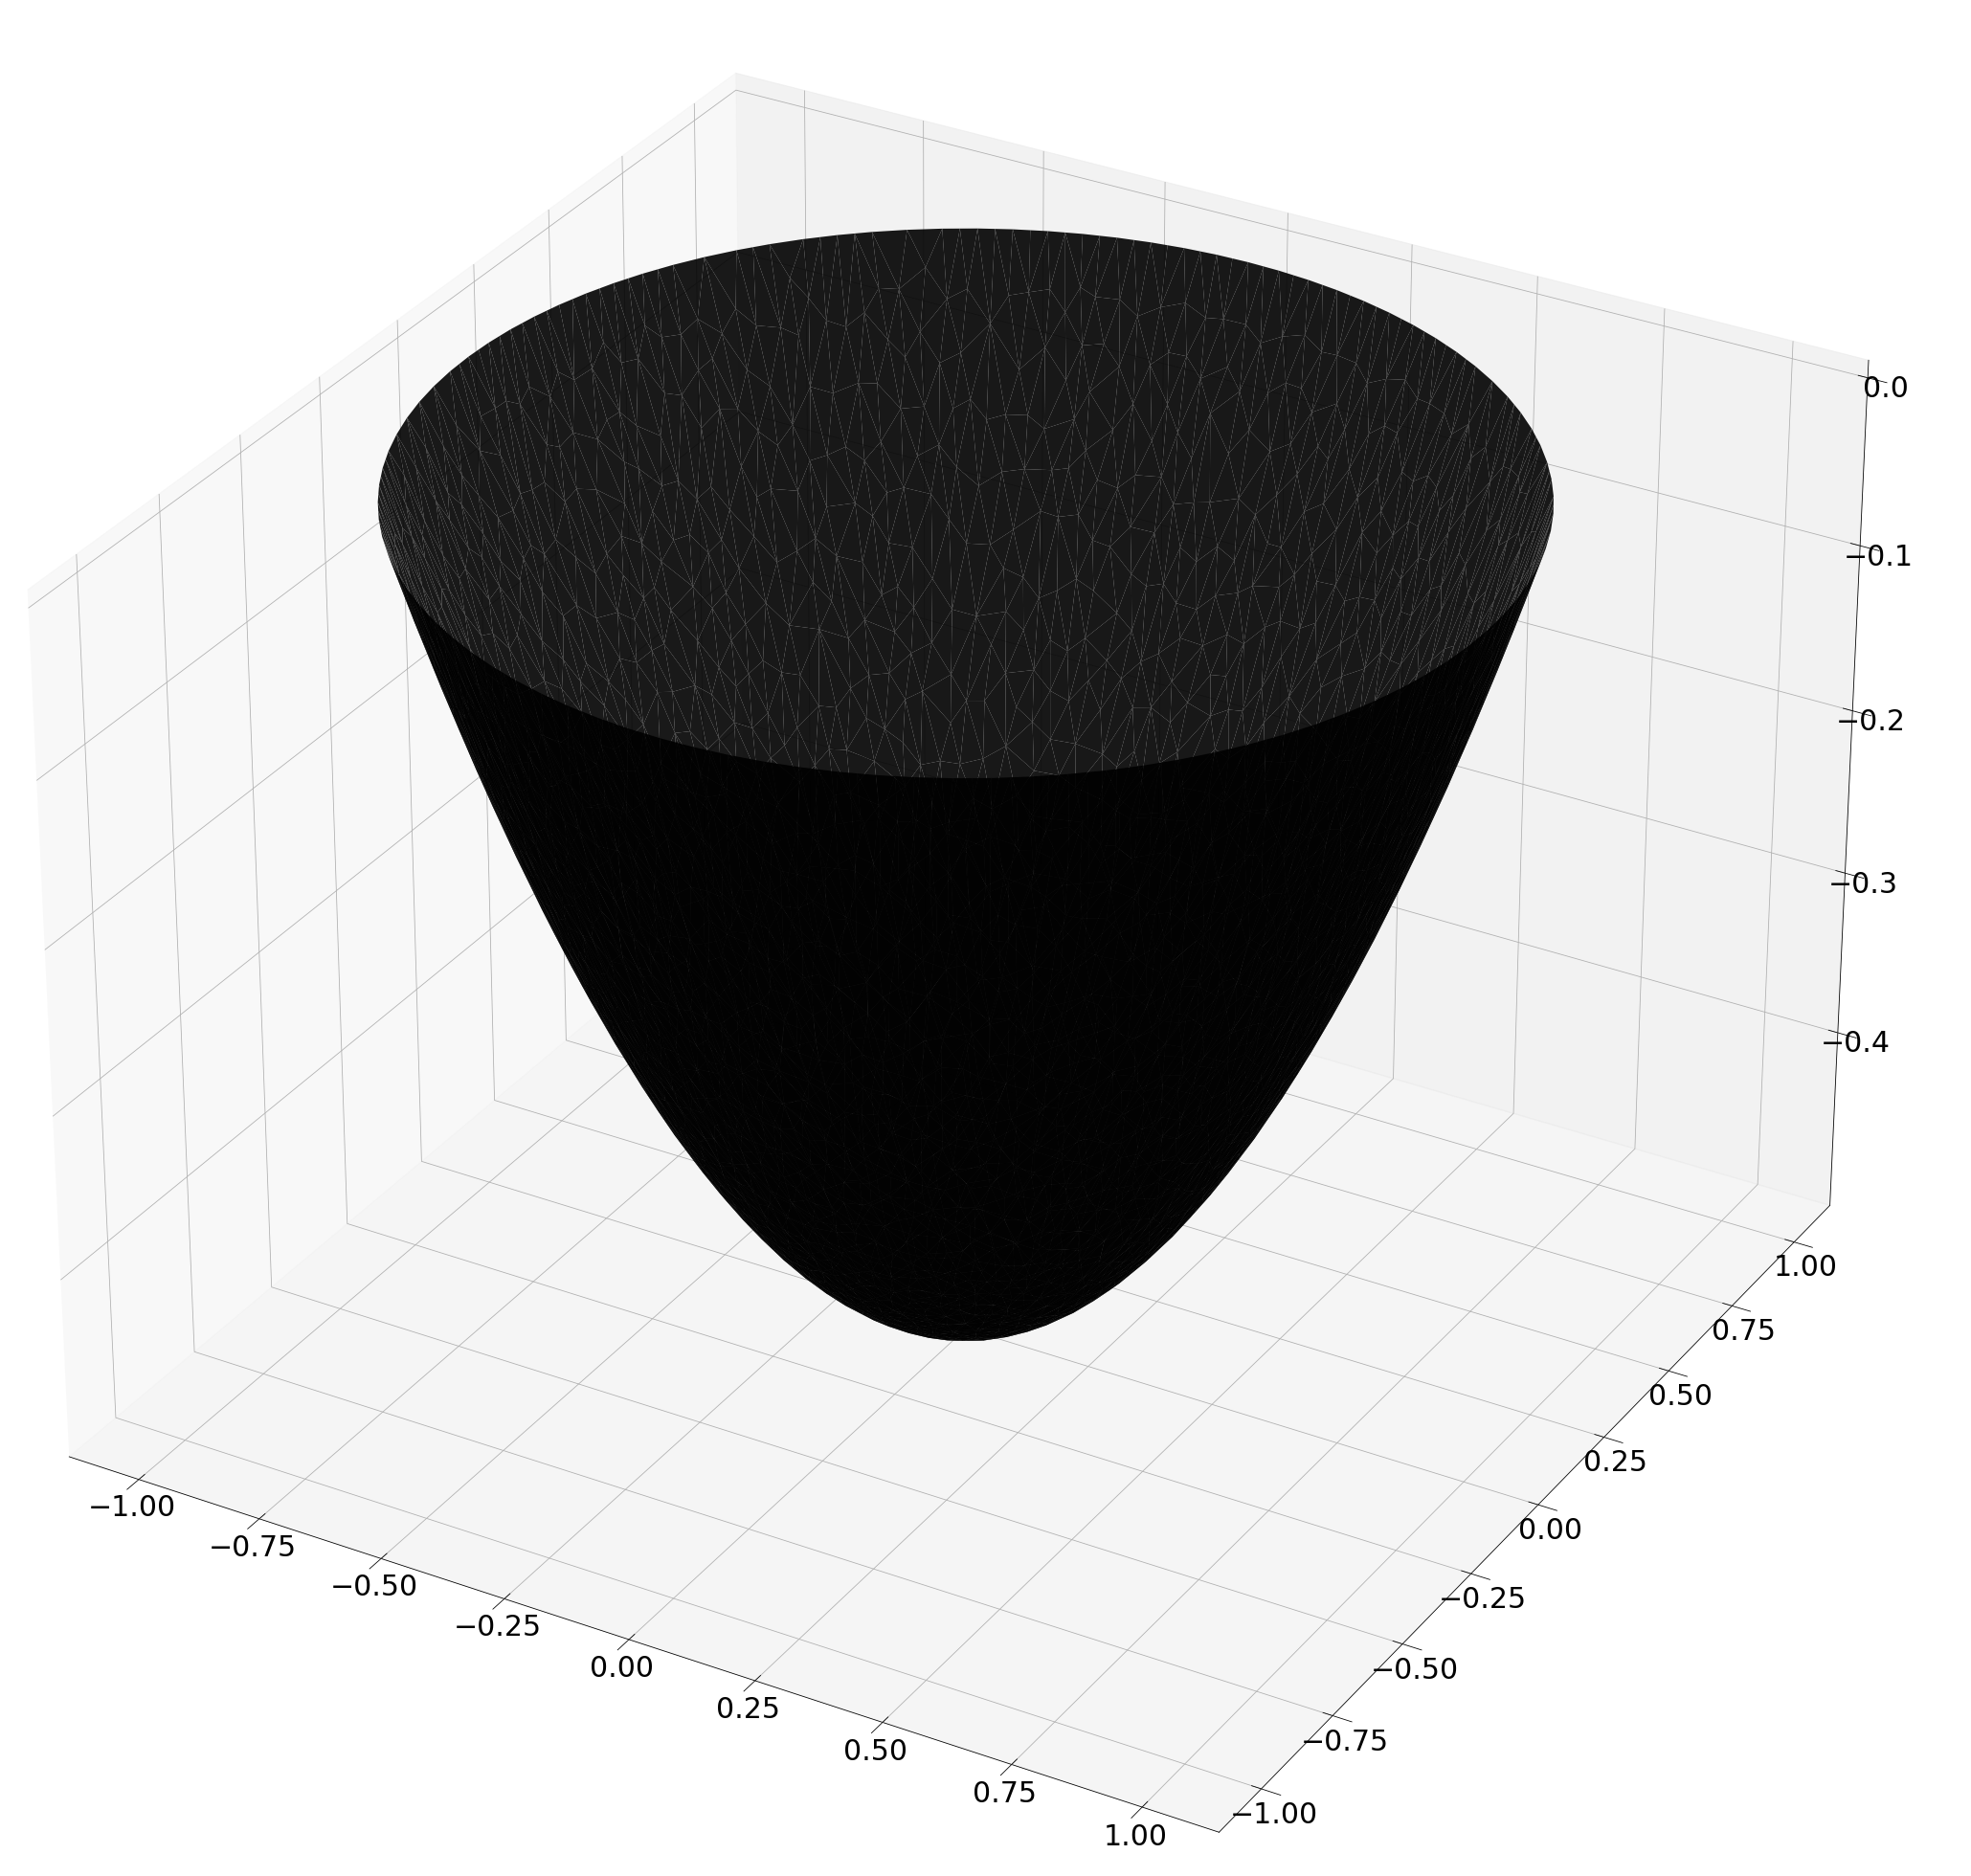
\includegraphics[width=0.8\textwidth]{images/poisson_equation_on_unit_circle_solution}
\captionsetup{labelformat=empty}
\caption{Նկար 4.4. Պուասոնի հավասարման լուծման գրաֆիկական ներկայացում։}
\end{figure}
\newpage
\subsection*{4.3 Բիհարմոնիկ հավասարման լուծում ուղղանկյուն տիրույթում}
Դիտարկենք հետևյալ դիֆերենցիալ հավասարումը.
\begin{equation}
\begin{dcases}
&\Delta^{2} u =f \\
&u \Big |_{\partial D} = 0\\
&\dfrac{\partial u}{\partial n} \Big |_{\partial D} = 0
\end{dcases}
\end{equation}
որտեղ $D = \left[x_{0}, x_{N}\right] \times \left[y_{0}, y_{M}\right]$:
Այս դիֆերենցիալ հավասարման  համապատասխան վարիացիոն խնդիրը կլինի.
\begin{equation}
I(u) = \frac{1}{2}\iint \limits_{D} \left[u_{xx}^{2} + 2u_{xy}^{2} + u_{yy}^{2} \right]dxdy - \iint \limits_{D} fudxdy \longrightarrow min
\end{equation}
$D$ տիրույթը տրոհենք ուղղանկյուների $h_{1}$ և $h_{2}$ քայլերով համապատասխանաբար ըստ $x$ և $y$ կոորդինատների։
Որոնելի ֆունկցիան կփնտրենք $\left(2.9\right)$ ում ներկայացված բազիսային ֆունկցիաների գծային կոմբինացիայի տեսքով.
\begin{equation}
u(x,y) = \sum_{i=0}^{N} \sum_{j=0}^{M} u_{ij}\varphi^{ij}(x,y)
\end{equation}
Հետևաբար ինտեգրալ ֆունկցիոնալը կունենք հետևյալ տեսքը.
\begin{equation}
$$\scalemath{0.7}{\frac{1}{2} \iint \limits_{D}\left[\left(\sum_{i=0}^{N} \sum_{j=0}^{M}u_{ij}\varphi^{ij}_{xx}(x,y)\right)^2 +  2\left(\sum_{i=0}^{N} \sum_{j=0}^{M}u_{ij}\varphi^{ij}_{xy}(x,y)\right)^2 + \left(\sum_{i=0}^{N} \sum_{j=0}^{M}u_{ij}\varphi^{ij}_{yy}(x,y)\right)^2\right]dxdy - \iint \limits_{D}f(x,y)\left[ \sum_{i=0}^{N} \sum_{j=0}^{M}u_{ij}\varphi^{ij}(x,y)\right]dxdy}
\end{equation}
Համաձայն էքստրեմումի անհրաժեշտ պայմանի.
\begin{equation}
\dfrac{\partial I}{ \partial u_{kl}} = \dfrac{\partial}{\partial u_{kl}} I \left(\sum_{j=0}^{M} u_{ij}\varphi^{ij}(x,y)\right) = 0
\end{equation}
Դիտարկենք $\left(18\right)$֊ի առաջին կրկնակի գումարը.
$$\left(\sum_{i=0}^{N} \sum_{j=0}^{M}u_{ij}\varphi_{xx}^{ij}(x,y)\right)^2 = \left[u_{kl}\varphi_{xx}^{kl}(x,y)\right]^{2} + 2u_{kl}\varphi_{xx}^{kl}(x,y)[\dots] + [\dots]^2$$
\noindent որտեղ բազմակետերով արտահայտությունը իր մեջ չի պարունակում $u_{kl}$ ը։
Հանգունորեն երկրորդ կրկնակի գումարի համար.
$$\left(\sum_{i=0}^{N} \sum_{j=0}^{M}u_{ij}\varphi_{xy}^{ij}(x,y)\right)^2 = \left[u_{kl}\varphi_{xy}^{kl}(x,y)\right]^{2} + 2u_{kl}\varphi_{xy}^{kl}(x,y)[\dots] + [\dots]^2$$
Հանգունորեն երրորդ կրկնակի գումարի համար.
$$\left(\sum_{i=0}^{N} \sum_{j=0}^{M}u_{ij}\varphi_{yy}^{ij}(x,y)\right)^2 = \left[u_{kl}\varphi_{yy}^{kl}(x,y)\right]^{2} + 2u_{kl}\varphi_{yy}^{kl}(x,y)[\dots] + [\dots]^2$$
Այսպիսով ավելի պարզեցված տեսքով համակարգը ունի հետևյալ տեսքը.

\begin{equation}\scalemath{0.65}{\frac{\partial}{\partial u_{kl}}I \left(u\right)= \iint \limits_{D} \left[2u_{kl}\left\{ \varphi_{xx}^{kl}(x,y)\right\}^{2} + 2\varphi_{xx}^{kl}(x,y)[\dots] + 4u_{kl}\left\{ \varphi_{xy}^{kl}(x,y)\right\}^{2} + 4\varphi_{xy}^{kl}(x,y)[\dots] + 2\left\{ \varphi_{yy}^{kl}(x,y)\right\}^{2} + 2u_{kl}\varphi_{yy}^{kl}(x,y)[\dots] + 2f(x,y)\varphi_{kl}(x,y)\right]dxdy}\end{equation}
Քանի որ տրված են Դիրիխլեի և Նեյմանի եզրային պայմանները, կդիտարկենք միայն $2 \leq k \leq M-2, 2 \leq l \leq N-2$ դեպքերը։
$\left(19\right)$ ինտեգրալը հաշվենք անդամ առ անդամ։
\begin{equation}
\iint \limits_{D} 2u_{kl}\left\{ \varphi_{xx}^{kl}(x,y)\right\}^{2}dxdy=2u_{kl}\int \limits_{x_{k-2}}^{x_{k+2}}\int \limits_{y_{l-2}}^{y_{l+2}} \left\{ B_{k}^{''}(x)B_{l}(y)\right\}^{2}dxdy=2u_{kl}\cdot \dfrac{6}{h_{1}^{3}} \cdot \dfrac{151}{140}h_{2}
\end{equation}
\begin{equation}\iint \limits_{D} 4u_{kl}\left\{ \varphi_{xy}^{kl}(x,y)\right\}^{2}dxdy=4u_{kl}\int \limits_{x_{k-2}}^{x_{k+2}}\int \limits_{y_{l-2}}^{y_{l+2}} \left\{ B_{k}^{'}(x)B_{l}^{'}(y)\right\}^{2}dxdy=4u_{kl}\cdot \dfrac{3}{2h_{1}} \cdot \dfrac{3}{2h_{2}}
\end{equation}
\begin{equation}
\iint \limits_{D} 2u_{kl}\left\{ \varphi_{yy}^{kl}(x,y)\right\}^{2}dxdy=2u_{kl}\int \limits_{x_{k-2}}^{x_{k+2}}\int \limits_{y_{l-2}}^{y_{l+2}} \left\{ B_{k}(x)B_{l}^{''}(y)\right\}^{2}dxdy=2u_{kl}\cdot \dfrac{151}{140}h_{2} \cdot \dfrac{6}{h_{1}^{3}}
\end{equation}
\begin{equation}
\begin{split}
\iint \limits_{D} 2f(x,y) \varphi^{kl}(x,y)dxdy = 2 \int \limits_{x_{k-2}}^{x_{k+2}}\int \limits_{y_{l-2}}^{y_{l+2}}f(x,y)B_{k}(x)B_{l}(y)dxdy\approx \\
\approx \dfrac{2}{9} h_{1}h_{2} \left[f_{k-1,l}+2f_{k,l}+f_{k+1,l}\right] \left[f_{k,l-1}+2f_{k,l}+f_{k,l+1}\right]
\end{split}
\end{equation}
Դիտարկենք մյուս ինտեգրալները։ Քանի որ $\varphi^{ij}$ բազիսային ֆունկցիաները ունեն լոկալ կրողներ $4 \times 4 = 16$ ուղղանկյուն էլեմենտներում, ապա տրված $\varphi^{kl}$ ֆունկցիան հատվում է 49 այլ բազիսային ֆունկցիաների հետ։ Բացառություն են կազմում $i=2, M-2$, $j=2, N-2$ դեպքերը, որոնց համար լոկալ կրողը $6 \times 7 = 42$ է եզրին հարող հանգույցների համար, և $6 \times 6 = 36$ անկյուններին հարող հանգույցների համար։ Ստորև ներկայացվում է երեք հնարավոր դեքերը (արտակատկերման համար ներկված հանգույցները պատկերված են ուղղանկյունների տեսքով)։
\begin{figure}[H]
  \centering
  \begin{minipage}[b]{0.2\textwidth}
    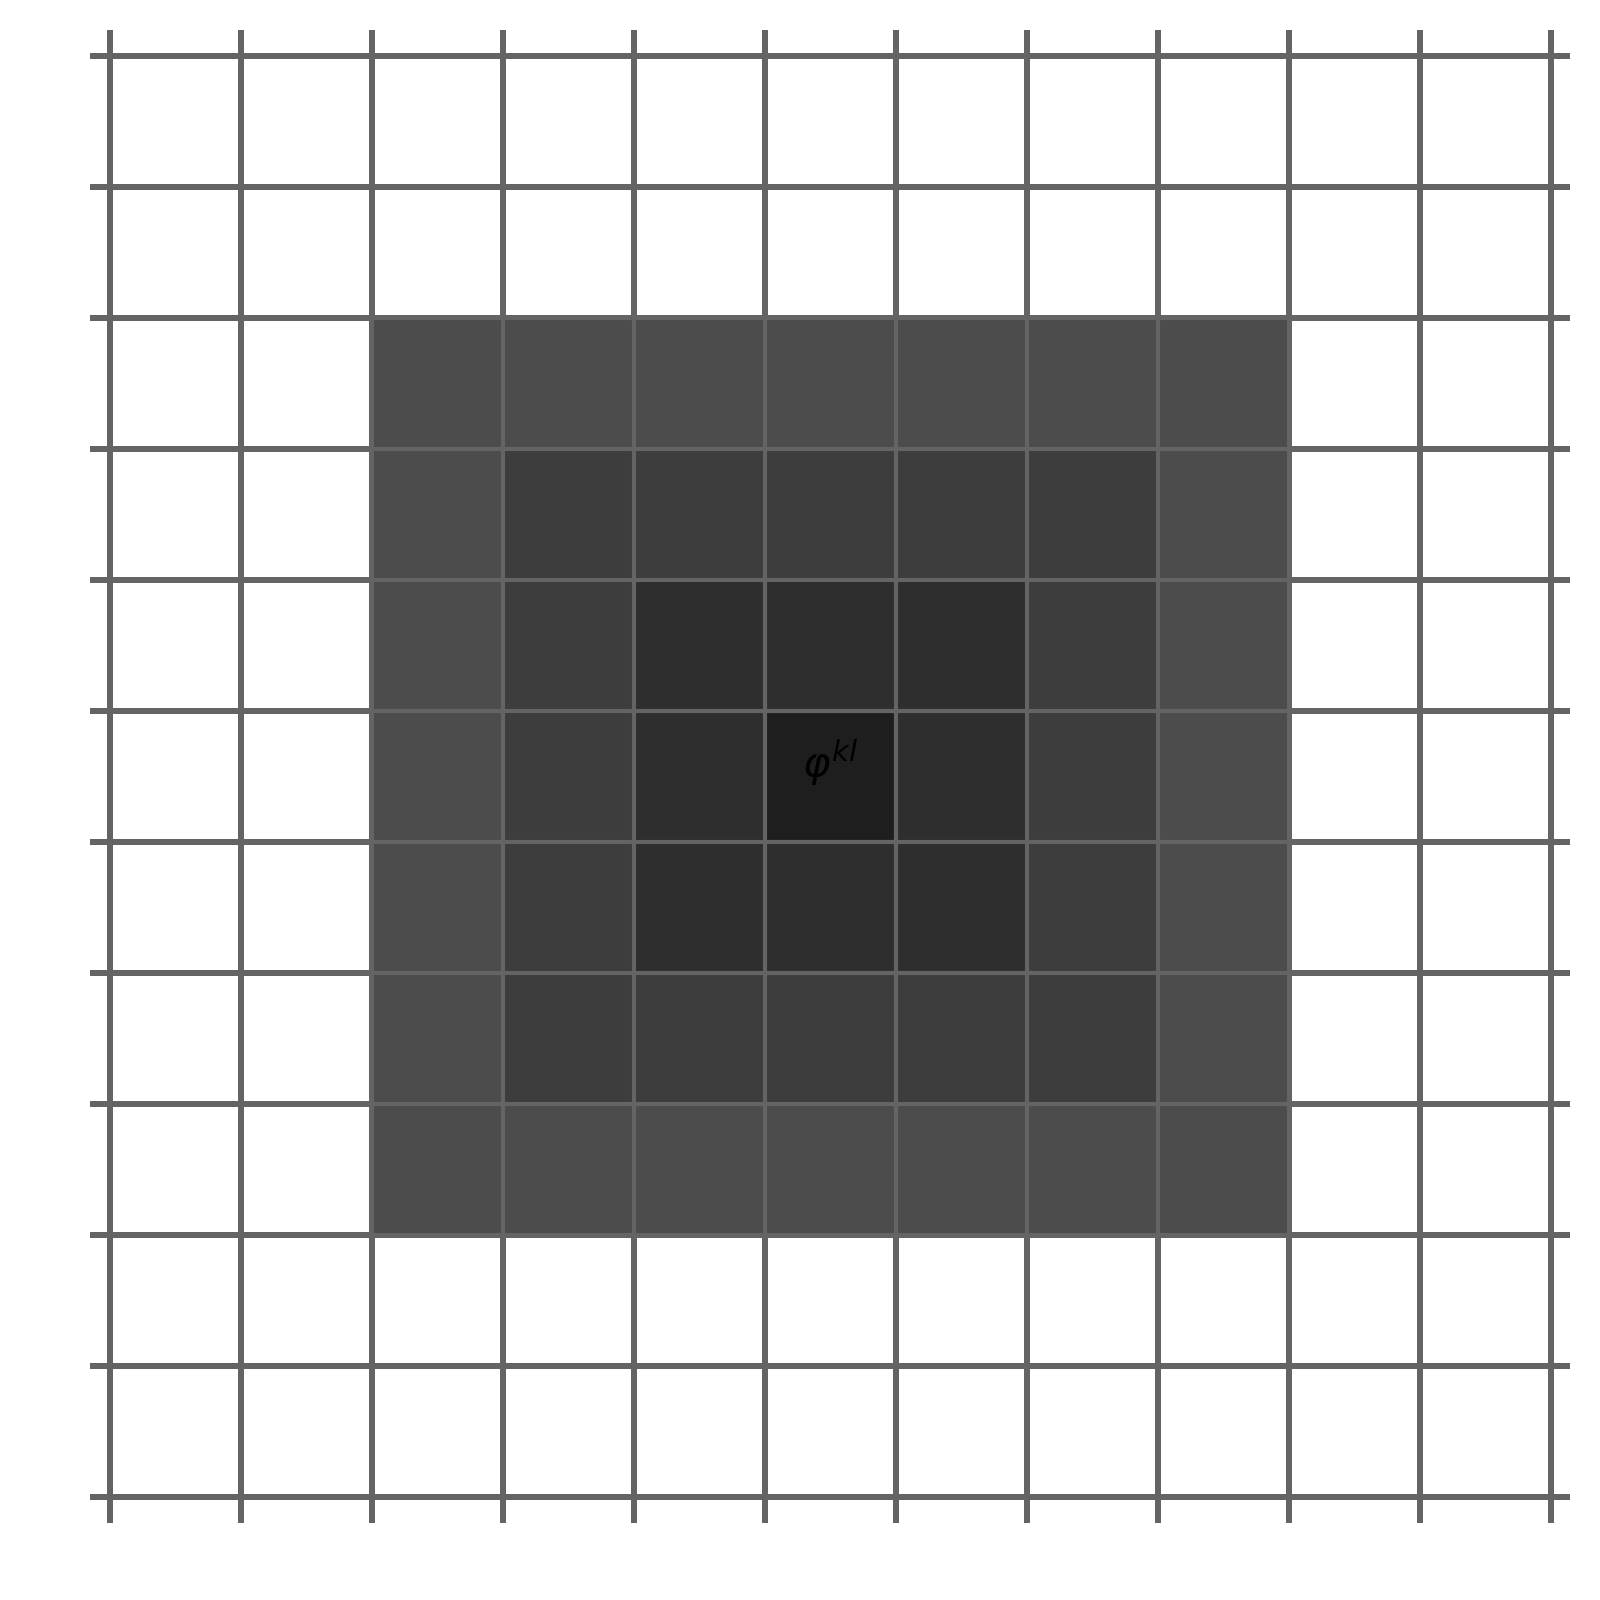
\includegraphics[width=\textwidth]{images/two_dimensional_basis_intersection}
    %\captionsetup{labelformat=empty}
  \end{minipage}
  \hfill
  \begin{minipage}[b]{0.2\textwidth}
    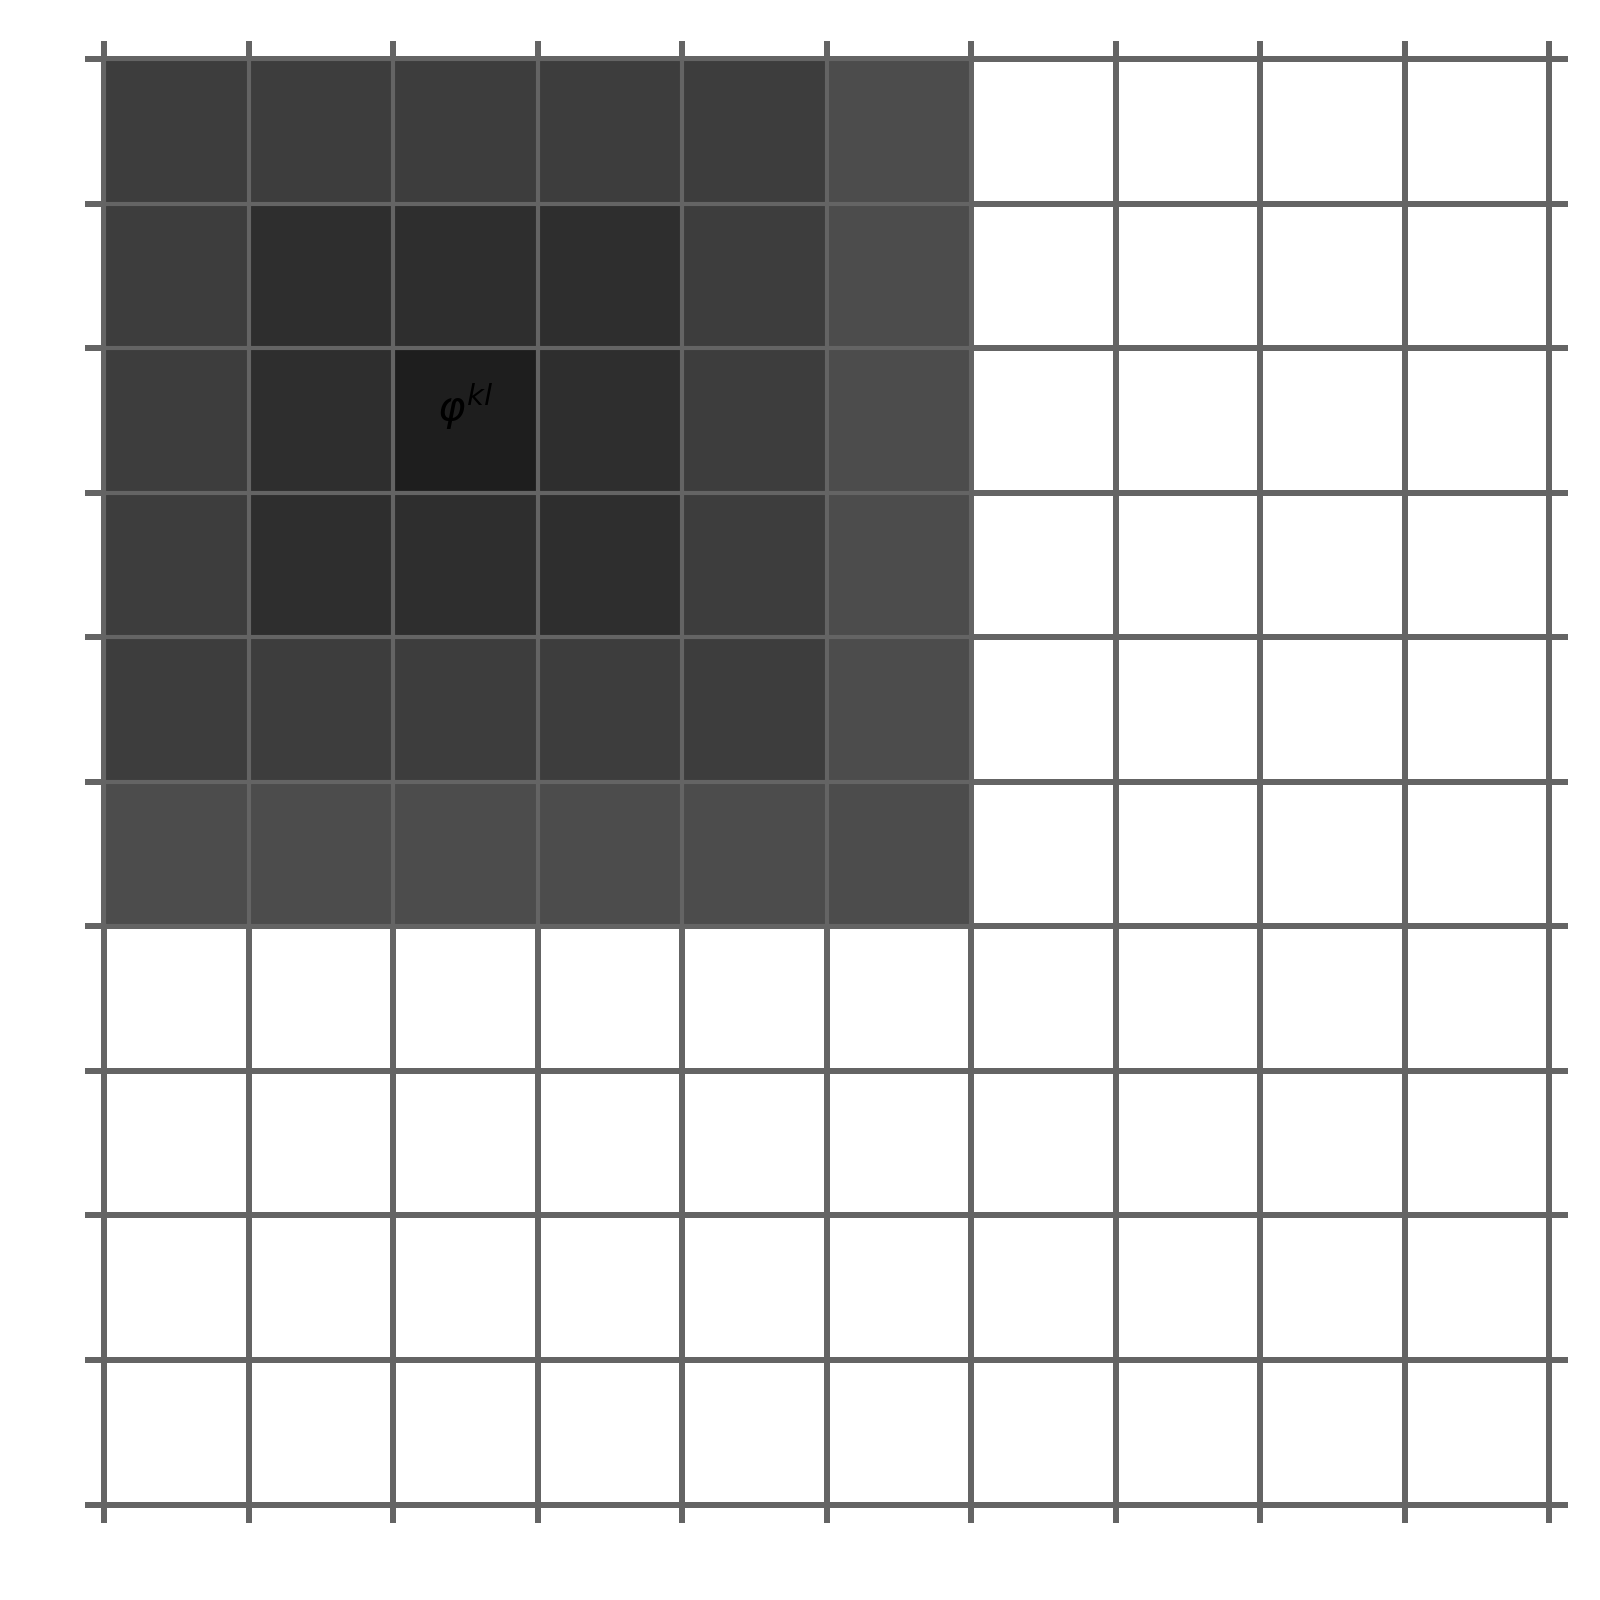
\includegraphics[width=\textwidth]{images/two_dimensional_basis_intersection_edge_1}
    %\captionsetup{labelformat=empty}
  \end{minipage}
\hfill
  \begin{minipage}[b]{0.2\textwidth}
    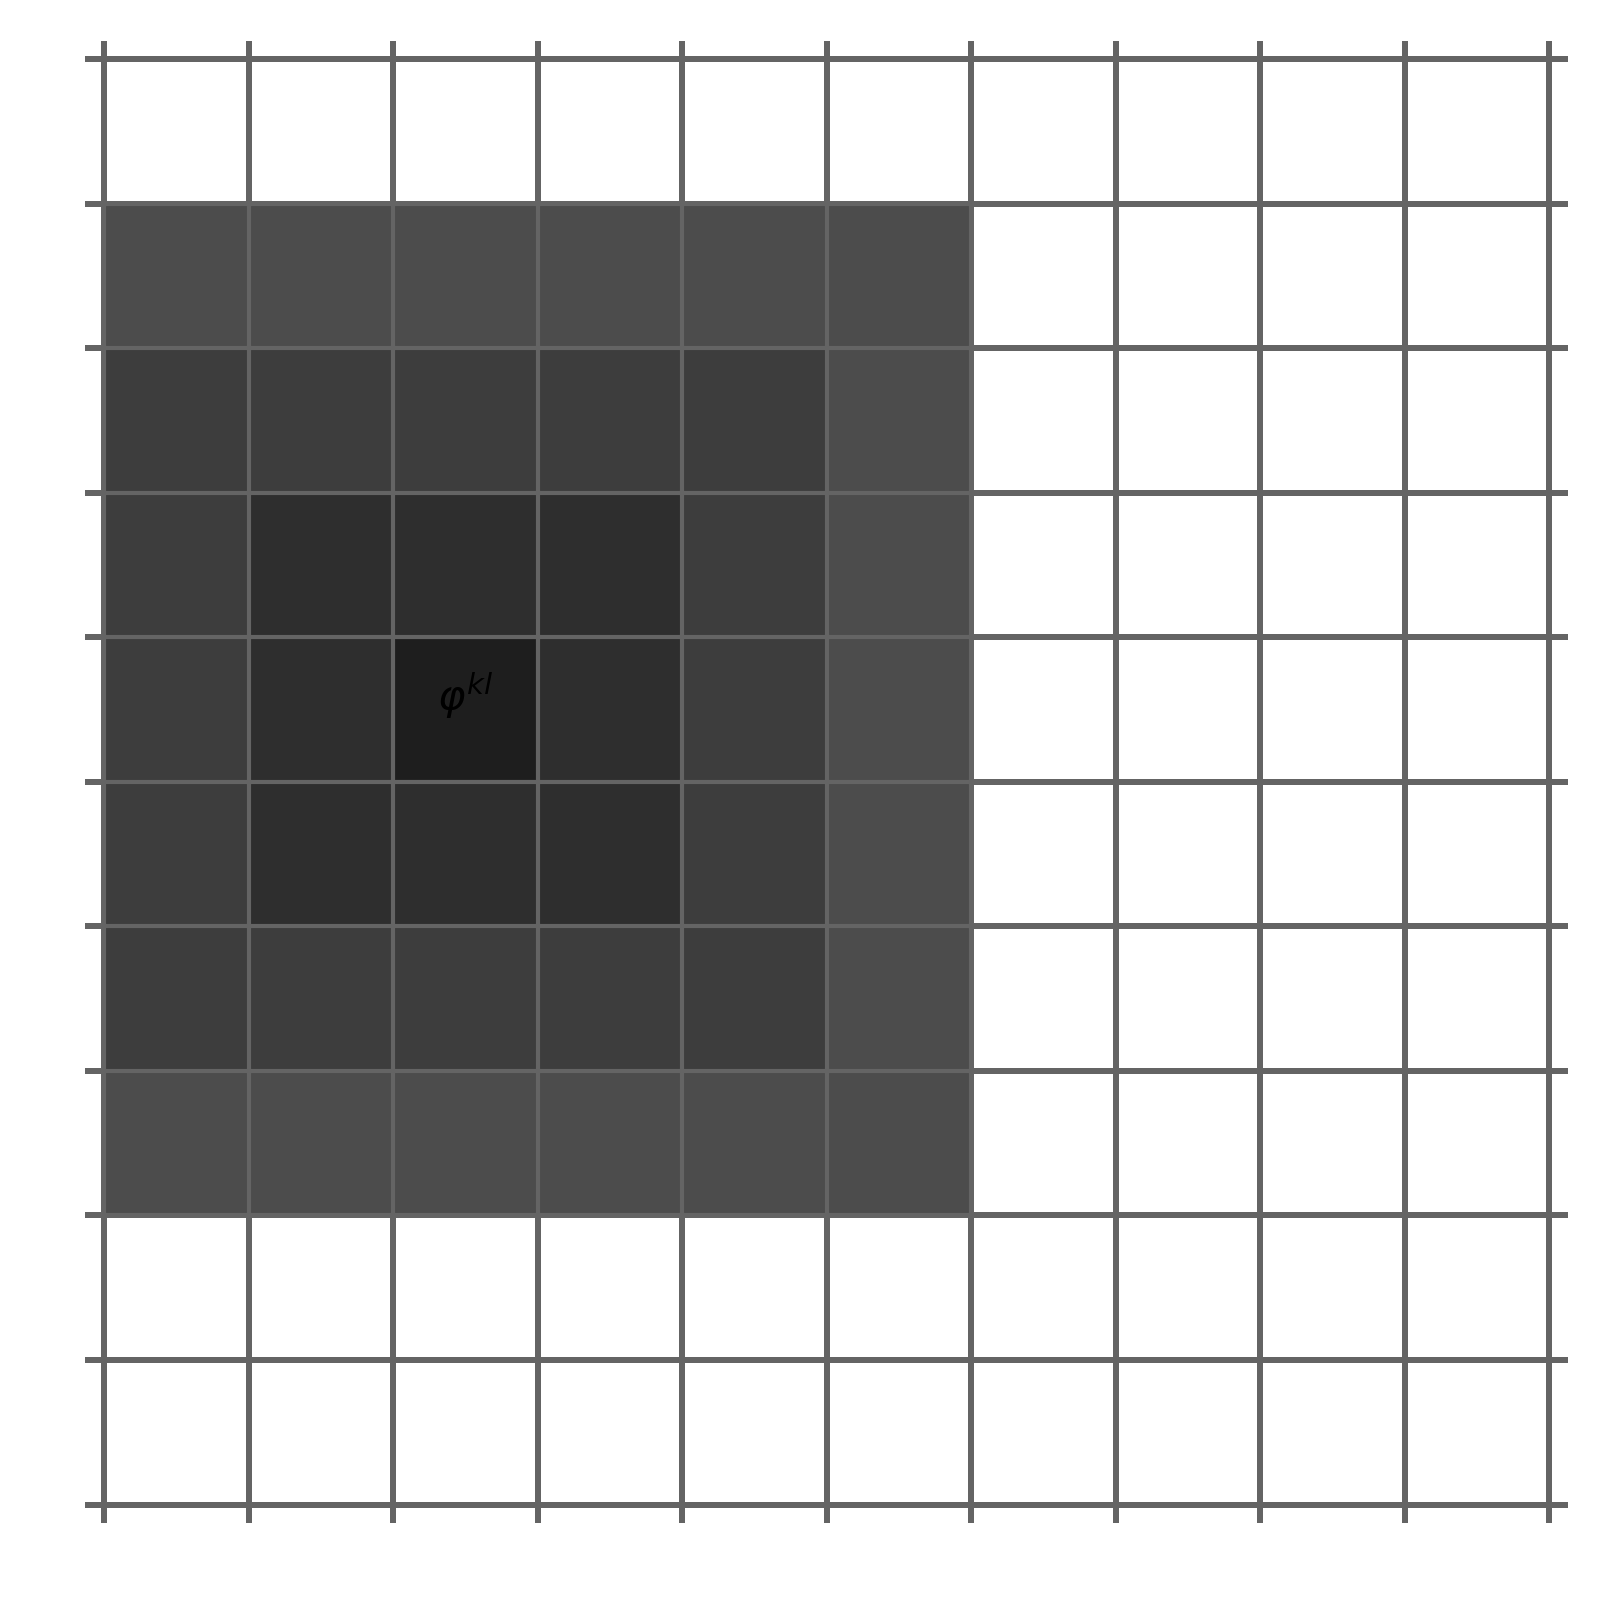
\includegraphics[width=\textwidth]{images/two_dimensional_basis_intersection_edge_2}
    %\captionsetup{labelformat=empty}
  \end{minipage}
\captionsetup{labelformat=empty}
\caption{Նկար 4.2. Բազիսային ֆունկցիաների հատումների ներկայացում տիրույթի ներսում, անկյունի վրա և եզրի վրա։}
\end{figure}
		$$\iint \limits_{D} 2\varphi_{xx}^{kl}(x,y)[\dots]dxdy, \iint \limits_{D} 4\varphi_{xy}^{kl}(x,y)[\dots]dxdy, \iint \limits_{D} 2\varphi_{yy}^{kl}(x,y)[\dots]dxdy$$
ինտեգրալները ներկայացնենք կրկնակի ինտեգրալների տեսքով։
\begin{equation}
\iint \limits_{D} 2\varphi_{xx}^{kl}(x,y)[\dots]dxdy= 2\sum_{\substack{i=k-3\\ i \neq k}}^{k+3}\sum_{\substack{j=l-3\\ j \neq l}}^{l+3} u_{ij}\int \limits_{x_{k-2}}^{x_{k+2}}B_{k}^{''}(x)B_{i}^{''}(x)dx \int \limits_{y_{l-2}}^{y_{l+2}}B_{l}(y)B_{j}(y)dy
\end{equation}
\begin{equation}
\iint \limits_{D} 4\varphi_{xy}^{kl}(x,y)[\dots]dxdy= 4\sum_{\substack{i=k-3\\ i \neq k}}^{k+3}\sum_{\substack{j=l-3\\ j \neq l}}^{l+3}u_{ij}\int \limits_{x_{k-2}}^{x_{k+2}}B_{k}^{'}(x)B_{i}^{'}(x)dx \int \limits_{y_{l-2}}^{y_{l+2}}B_{l}^{'}(y)B_{j}^{'}(y)dy
\end{equation}
\begin{equation}
\iint \limits_{D} 2\varphi_{yy}^{kl}(x,y)[\dots]dxdy= 2\sum_{\substack{i=k-3\\ i \neq k}}^{k+3}\sum_{\substack{j=l-3\\ j \neq l}}^{l+3}u_{ij}\int \limits_{x_{k-2}}^{x_{k+2}}B_{k}(x)B_{i}(x)dx \int \limits_{y_{l-2}}^{y_{l+2}}B_{l}^{''}(y)B_{j}^{''}(y)dy
\end{equation}
\newpage
Դիտարկենք  հետևյալ դեպքերը.
\begin{enumerate}
\item{Երբ $3 \leq k \leq M-3, \; 3 \leq l \leq N-3$ }

Առաջին ինտեգրալի համար
\begin{equation}
\begin{aligned}
&\int \limits_{x_{k-2}}^{x_{k+2}}B_{k}^{''}(x)B_{k-3}^{''}(x)dx = \dfrac{3}{8h_{1}^3}, \; \int \limits_{x_{k-2}}^{x_{k+2}}B_{k}^{''}(x)B_{k-2}^{''}(x)dx = 0, \; \int \limits_{x_{k-2}}^{x_{k+2}}B_{k}^{''}(x)B_{k-1}^{''}(x)dx = -\dfrac{27}{8h_{1}^3} \\
&\int \limits_{x_{k-2}}^{x_{k+2}}B_{k}^{''}(x)B_{k+1}^{''}(x)dx =-\dfrac{27}{8h_{1}^3}, \; \int \limits_{x_{k-2}}^{x_{k+2}}B_{k}^{''}(x)B_{k+2}^{''}(x)dx = 0, \; \int \limits_{x_{k-2}}^{x_{k+2}}B_{k}^{''}(x)B_{k+3}^{''}(x)dx =  \dfrac{3}{8h_{1}^3} \\
&\int \limits_{y_{l-2}}^{y_{l+2}}B_{l}(y)B_{l-3}(y)dy=\dfrac{h_{2}}{2240}, \; \int \limits_{y_{l-2}}^{y_{l+2}}B_{l}(y)B_{l-2}(y)dy=\dfrac{3h_{2}}{56}, \; \int \limits_{y_{l-2}}^{y_{l+2}}B_{l}(y)B_{l-1}(y)dy=\dfrac{1991h_{2}}{2240} \\
&\int \limits_{y_{l-2}}^{y_{l+2}}B_{l}(y)B_{l+1}(y)dy=\dfrac{1991h_{2}}{2240}, \; \int \limits_{y_{l-2}}^{y_{l+2}}B_{l}(y)B_{l+2}(y)dy=\dfrac{3h_{2}}{56}, \; \int \limits_{y_{l-2}}^{y_{l+2}}B_{l}(y)B_{l+3}(y)dy=\dfrac{h_{2}}{2240}
\end{aligned}
\end{equation}
Երկրորդ ինտեգրալի համար
\begin{equation}
\begin{aligned}
&\int \limits_{x_{k-2}}^{x_{k+2}}B_{k}^{'}(x)B_{k-3}^{'}(x)dx=\dfrac{-3}{160h_{1}}, \; \int \limits_{x_{k-2}}^{x_{k+2}}B_{k}^{'}(x)B_{k-2}^{'}(x)dx=\dfrac{-9}{20h_{1}}, \; \int \limits_{x_{k-2}}^{x_{k+2}}B_{k}^{'}(x)B_{k-1}^{'}(x)dx=\dfrac{-9}{32h_{1}} \\
&\int \limits_{x_{k-2}}^{x_{k+2}}B_{k}^{'}(x)B_{k+1}^{'}(x)dx=\dfrac{-9}{32h_{1}}, \; \int \limits_{x_{k-2}}^{x_{k+2}}B_{k}^{'}(x)B_{k+2}^{'}(x)dx=\dfrac{-9}{20h_{1}}, \; \int \limits_{x_{k-2}}^{x_{k+2}}B_{k}^{'}(x)B_{k+3}^{'}(x)dx=\dfrac{-3}{160h_{1}} \\
&\int \limits_{y_{l-2}}^{y_{l+2}}B_{l}^{'}(y)B_{l-3}^{'}(y)dy=\dfrac{-3}{160h_{2}}, \; \int \limits_{y_{l-2}}^{y_{l+2}}B_{l}^{'}(y)B_{l-2}^{'}(y)dy=\dfrac{-9}{20h_{2}}, \; \int \limits_{y_{l-2}}^{y_{l+2}}B_{l}^{'}(y)B_{l-1}^{'}(y)dy=\dfrac{-9}{32h_{2}} \\
&\int \limits_{y_{l-2}}^{y_{l+2}}B_{l}^{'}(y)B_{l+1}^{'}(y)dy=\dfrac{-9}{32h_{2}}, \; \int \limits_{y_{l-2}}^{y_{l+2}}B_{l}^{'}(y)B_{l+2}^{'}(y)dy=\dfrac{-9}{20h_{2}}, \; \int \limits_{y_{l+2}}^{y_{l+2}}B_{l}^{'}(y)B_{l+3}^{'}(y)dy=\dfrac{-3}{160h_{2}}
\end{aligned}
\end{equation}
Երրորդ ինտեգրալի համար
\begin{equation}
\begin{aligned}
&\int \limits_{x_{k-2}}^{x_{k+2}}B_{k}(x)B_{k-3}(x)dx=\dfrac{h_{1}}{2240}, \; \int \limits_{x_{k-2}}^{x_{k+2}}B_{k}(x)B_{k-2}(x)dx=\dfrac{3h_{1}}{56}, \; \int \limits_{x_{k-2}}^{x_{k+2}}B_{k}(x)B_{k-1}(x)dx=\dfrac{1991h_{1}}{2240} \\
&\int \limits_{x_{k-2}}^{x_{k+2}}B_{k}(x)B_{k+1}(x)dx=\dfrac{1991h_{1}}{2240}, \; \int \limits_{x_{k-2}}^{x_{l+2}}B_{k}(x)B_{k+2}(x)dx=\dfrac{3h_{1}}{56}, \; \int \limits_{x_{k-2}}^{x_{k+2}}B_{k}(x)B_{k+3}(x)dx=\dfrac{h_{1}}{2240} \\
&\int \limits_{y_{l-2}}^{y_{l+2}}B_{l}^{''}(y)B_{l-3}^{''}(y)dy = \dfrac{3}{8h_{2}^3}, \; \int \limits_{y_{l-2}}^{y_{l+2}}B_{l}^{''}(y)B_{l-2}^{''}(y)dy = 0, \; \int \limits_{y_{l-2}}^{y_{l+2}}B_{l}^{''}(y)B_{l-1}^{''}(y)dy = -\dfrac{27}{8h_{2}^3} \\
&\int \limits_{y_{l-2}}^{y_{l+2}}B_{l}^{''}(y)B_{l+1}^{''}(y)dy =-\dfrac{27}{8h_{2}^3}, \; \int \limits_{y_{l-2}}^{y_{l+2}}B_{l}^{''}(y)B_{l+2}^{''}(y)dy = 0, \; \int \limits_{y_{l-2}}^{y_{l+2}}B_{l}^{''}(y)B_{l+3}^{''}(y)dy =  \dfrac{3}{8h_{2}^3}
\end{aligned}
\end{equation}
\item{$k=2,  l =2 $}

Առաջին ինտեգրալի համար
\begin{equation}
\begin{aligned}
&\int \limits_{x_{0}}^{x_{4}}B_{2}^{''}(x)B_{0}^{''}(x)dx = \dfrac{3}{8h_{1}^3}, \; \int \limits_{x_{0}}^{x_{4}}B_{2}^{''}(x)B_{1}^{''}(x)dx = -\dfrac{27}{8h_{1}^3} \\
&\int \limits_{x_{0}}^{x_{4}}B_{2}^{''}(x)B_{3}^{''}(x)dx =-\dfrac{27}{8h_{1}^3}, \; \int \limits_{x_{0}}^{x_{4}}B_{2}^{''}(x)B_{4}^{''}(x)dx = 0, \; \int \limits_{x_{0}}^{x_{4}}B_{2}^{''}(x)B_{5}^{''}(x)dx =  \dfrac{3}{8h_{1}^3} \\
&\int \limits_{y_{0}}^{y_{4}}B_{2}(y)B_{0}(y)dy=\dfrac{121h_{2}}{2240}, \; \int \limits_{y_{0}}^{y_{4}}B_{2}(y)B_{1}(y)dy=\dfrac{1991h_{2}}{2240} \\
&\int \limits_{y_{0}}^{y_{4}}B_{2}(y)B_{3}(y)dy=\dfrac{1991h_{2}}{2240}, \; \int \limits_{y_{0}}^{y_{4}}B_{l}(y)B_{4}(y)dy=\dfrac{3h_{2}}{56}, \; \int \limits_{y_{0}}^{y_{4}}B_{l}(y)B_{l+3}(y)dy=\dfrac{h_{2}}{2240}
\end{aligned}
\end{equation}
Երկրորդ ինտեգրալի համար
\begin{equation}
\begin{aligned}
&\int \limits_{x_{0}}^{x_{4}}B_{2}^{'}(x)B_{0}^{'}(x)dx=-\dfrac{15}{32h_{1}}, \; \int \limits_{x_{0}}^{x_{4}}B_{2}^{'}(x)B_{1}^{'}(x)dx=-\dfrac{9}{32h_{1}} \\
&\int \limits_{x_{0}}^{x_{4}}B_{2}^{'}(x)B_{3}^{'}(x)dx=\dfrac{-9}{32h_{1}}, \; \int \limits_{x_{0}}^{x_{4}}B_{k}^{'}(x)B_{3}^{'}(x)dx=\dfrac{-9}{20h_{1}}, \; \int \limits_{x_{0}}^{x_{4}}B_{k}^{'}(x)B_{5}^{'}(x)dx=\dfrac{-3}{160h_{1}} \\
&\int \limits_{y_{0}}^{y_{4}}B_{2}^{'}(y)B_{0}^{'}(y)dy=-\dfrac{9}{32h_{2}}, \; \int \limits_{y_{0}}^{y_{4}}B_{l}^{'}(y)B_{1}^{'}(y)dy=-\dfrac{9}{32h_{2}} \\
&\int \limits_{y_{0}}^{y_{4}}B_{2}^{'}(y)B_{3}^{'}(y)dy=\dfrac{-9}{32h_{2}}, \; \int \limits_{y_{0}}^{y_{4}}B_{l}^{'}(y)B_{3}^{'}(y)dy=\dfrac{-9}{20h_{2}}, \; \int \limits_{y_{0}}^{y_{4}}B_{l}^{'}(y)B_{5}^{'}(y)dy=\dfrac{-3}{160h_{2}}
\end{aligned}
\end{equation}
Երրորդ ինտեգրալի համար
\begin{equation}
\begin{aligned}
&\int \limits_{x_{0}}^{x_{4}}B_{2}(x)B_{0}(x)dx=\dfrac{121h_{1}}{2240}, \; \int \limits_{x_{0}}^{x_{4}}B_{2}(x)B_{1}(x)dx=\dfrac{1991h_{1}}{2240} \\
&\int \limits_{x_{0}}^{x_{4}}B_{2}(x)B_{3}(x)dx=\dfrac{1991h_{1}}{2240}, \; \int \limits_{x_{0}}^{x_{4}}B_{2}(x)B_{4}(x)dx=\dfrac{3h_{1}}{56}, \; \int \limits_{x_{0}}^{x_{4}}B_{2}(x)B_{5}(x)dx=\dfrac{h_{1}}{2240} \\
&\int \limits_{y_{0}}^{y_{4}}B_{2}^{''}(y)B_{0}^{''}(y)dy = -\dfrac{3}{8h_{1}^{2}}, \; \int \limits_{y_{0}}^{y_{4}}B_{2}^{''}(y)B_{1}^{''}(y)dy = -\dfrac{27}{8h_{2}^3} \\
&\int \limits_{y_{0}}^{y_{4}}B_{2}^{''}(y)B_{3}^{''}(y)dy =-\dfrac{27}{8h_{2}^3}, \; \int \limits_{y_{0}}^{y_{4}}B_{2}^{''}(y)B_{4}^{''}(y)dy = 0, \; \int \limits_{y_{0}}^{y_{4}}B_{2}^{''}(y)B_{5}^{''}(y)dy =  \dfrac{3}{8h_{2}^3}
\end{aligned}
\end{equation}
\item{$k=M-2, l=N-2$}
Քանի որ բազիսային ֆունկցիաները սիմետրիկ են, ապա այդ դեպքում կատարվում են նույն հաշվարկները, ինչ նախորդ կետում։
\end{enumerate}
Հաշվի առնելով նախորդիվ հաշվարկված ինտեգրալները, ինչպես նաև Դիրիխլեի և Նեյմանի եզրային պայմանները, կստանանք հետևյալ հավասարումենրի համակարգը.
Դիրիխլեի եզրային պայմաններ.
\begin{equation}
\begin{dcases}
u_{00}+\frac{5}{16}(u_{01} + u_{10}) +\frac{1}{16}u_{11} &= 0\\
u_{M0}+\frac{5}{16}(u_{M1} + u_{M-1,0}) +\frac{1}{16}u_{M-1, 1} &= 0\\
u_{0N}+\frac{5}{16}(u_{1N} + u_{0,N-1}) +\frac{1}{16}u_{N-1, 1} &= 0\\
u_{MN}+\frac{5}{16}(u_{M-1,N} + u_{M,N-1}) +\frac{1}{16}u_{M-1,N-1} &= 0
\end{dcases}
\end{equation}
Նեյմանի եզրային պայմաններ.
\begin{equation}
\begin{dcases}
\dfrac{3}{4h_{2}}\left(u_{i1} - u_{i0}\right) + \dfrac{3}{16h_{2}}\left(u_{i-1, 0}+u_{i+1, 0}+u_{i-1, 1}+u_{i+1, 1}\right)&=0\\
\dfrac{3}{4h_{2}}\left(u_{iN} - u_{i, N-1}\right) + \dfrac{3}{16h_{2}}\left(u_{i-1, N-1}+u_{i+1, N-1}+u_{i-1, N-1}+u_{i+1, N-1}\right)&=0\\
\dfrac{3}{4h_{1}}\left(u_{1j} - u_{0j}\right) + \dfrac{3}{16h_{1}}\left(u_{0, j-1}+u_{0, j+1}+u_{1, j-1}+u_{1, j+1}\right)&=0\\
\dfrac{3}{4h_{1}}\left(u_{Mj} - u_{M-1,j}\right) + \dfrac{3}{16h_{1}}\left(u_{M-1,j-1}+u_{M-1, j+1}+u_{M-1, j-1}+u_{M-1, j+1}\right)&=0\\
\end{dcases}
\end{equation}
Մինիմումի պայմաններ.
\begin{equation}
\begin{gathered}
\scalemath{0.6}{
\left(
 \begin{bmatrix}
           \sfrac{3}{8h_{1}^{2}} \\
           0 \\
           -\sfrac{27}{8h_{1}^{3}} \\
	\sfrac{6}{h_{1}^{3}} \\
           -\sfrac{27}{8h_{1}^{3}} \\
           0 \\
           \sfrac{3}{8h_{1}^{2}} \\
\end{bmatrix} \otimes \begin{bmatrix}
           \sfrac{h_{2}}{2240} \\
           \sfrac{3h_{2}}{56} \\
           \sfrac{1991h_{2}}{2240} \\
	 \sfrac{151h_{2}}{140} \\
           \sfrac{1991h_{2}}{2240} \\
           \sfrac{3h_{2}}{56} \\
           \sfrac{h_{2}}{2240}\\
\end{bmatrix} 
+
 \begin{bmatrix}
           -\sfrac{3}{160h_{1}} \\
           -\sfrac{9}{20h_{1}} \\
	-\sfrac{9}{32h_{1}} \\
           \sfrac{3}{2h_{1}} \\
	-\sfrac{9}{32h_{1}} \\
           -\sfrac{9}{20h_{1}} \\
           -\sfrac{3}{160h_{1}} \\
\end{bmatrix} \otimes  \begin{bmatrix}
           -\sfrac{3}{160h_{1}} \\
           -\sfrac{9}{20h_{1}} \\
	-\sfrac{9}{32h_{1}} \\
           \sfrac{3}{2h_{1}} \\
	-\sfrac{9}{32h_{1}} \\
           -\sfrac{9}{20h_{1}} \\
           -\sfrac{3}{160h_{1}} \\
\end{bmatrix} 
+ 
 \begin{bmatrix}
           \sfrac{h_{2}}{2240} \\
           \sfrac{3h_{2}}{56} \\
           \sfrac{1991h_{2}}{2240} \\
	 \sfrac{151h_{2}}{140} \\
           \sfrac{1991h_{2}}{2240} \\
           \sfrac{3h_{2}}{56} \\
           \sfrac{h_{2}}{2240}\\
\end{bmatrix}\otimes \begin{bmatrix}
           \sfrac{3}{8h_{1}^{2}} \\
           0 \\
           -\sfrac{27}{8h_{1}^{3}} \\
	\sfrac{6}{h_{1}^{3}} \\
           -\sfrac{27}{8h_{1}^{3}} \\
           0 \\
           \sfrac{3}{8h_{1}^{2}} \\
\end{bmatrix}
\right)
\begin{bmatrix}
u_{k-3,l-3} & u_{k-2,l-3} & u_{k-1,l-3} & u_{k,l-3} & u_{k+1,l-3} & u_{k+2,l-3} & u_{k+3,l-3}\\
u_{k-3,l-2} & u_{k-2,l-2} & u_{k-1,l-2} & u_{k,l-2} & u_{k+1,l-2} & u_{k+2,l-2} & u_{k+3,l-2}\\
u_{k-3,l-1} & u_{k-2,l-1} & u_{k-1,l-1} & u_{k,l-1} & u_{k+1,l-1} & u_{k+2,l-1} & u_{k+3,l-1}\\
u_{k-3,l} & u_{k-2,l} & u_{k-1,l} & u_{k,l} & u_{k+1,l} & u_{k+2,l} & u_{k+3,l}\\
u_{k-3,l+1} & u_{k-2,l+1} & u_{k-1,l+1} & u_{k,l+1} & u_{k+1,l+1} & u_{k+2,l+1} & u_{k+3,l+1}\\
u_{k-3,l+2} & u_{k-2,l+2} & u_{k-1,l+2} & u_{k,l+2} & u_{k+1,l+2} & u_{k+2,l+2} & u_{k+3,l+2}\\
u_{k-3,l+3} & u_{k-2,l+3} & u_{k-1,l+3} & u_{k,l+3} & u_{k+1,l+3} & u_{k+2,l+3} & u_{k+3,l+3}\\
\end{bmatrix}}=\\ 
=\dfrac{2}{9} h_{1}h_{2} \left[f_{k-1,l}+2f_{k,l}+f_{k+1,l}\right] \left[f_{k,l-1}+2f_{k,l}+f_{k,l+1}\right] 
\end{gathered}
\end{equation}
$k=2, M-2$, ինչպես նաև $l=2, N-2$ ֊ի համար կազմվում է նույն հավասարումը, փոխելով միայն համապասխան գործակիցները և դրանց քանակը։
\newpage
\subsubsection*{Ծրագրային իրականացում}
Ինչպես Պուասոնի հավասարման դեպքում, այնպես էլ այս դեպքում կօգտվենք նույն գործիքներից։
Որպես օրինակ լուծենք հետևյալ հավասարումը տրված կոնկրետ տիրույթով և $f$ ֆունկցիայով։
$$\begin{dcases}
								\Delta^{2} u &=1 \\
								u \Big |_{\partial D} &= 0\\
								\dfrac{\partial u}{\partial n} \Big |_{\partial D} &= 0
\end{dcases}$$
որտեղ $D = \left[0, 1\right] \times \left[-1, 1\right], \; h_{1}=0.01, h_{2}=0.02$։

Խնդրի համար ստացված լուծումը.
\begin{figure}[H]
\centering
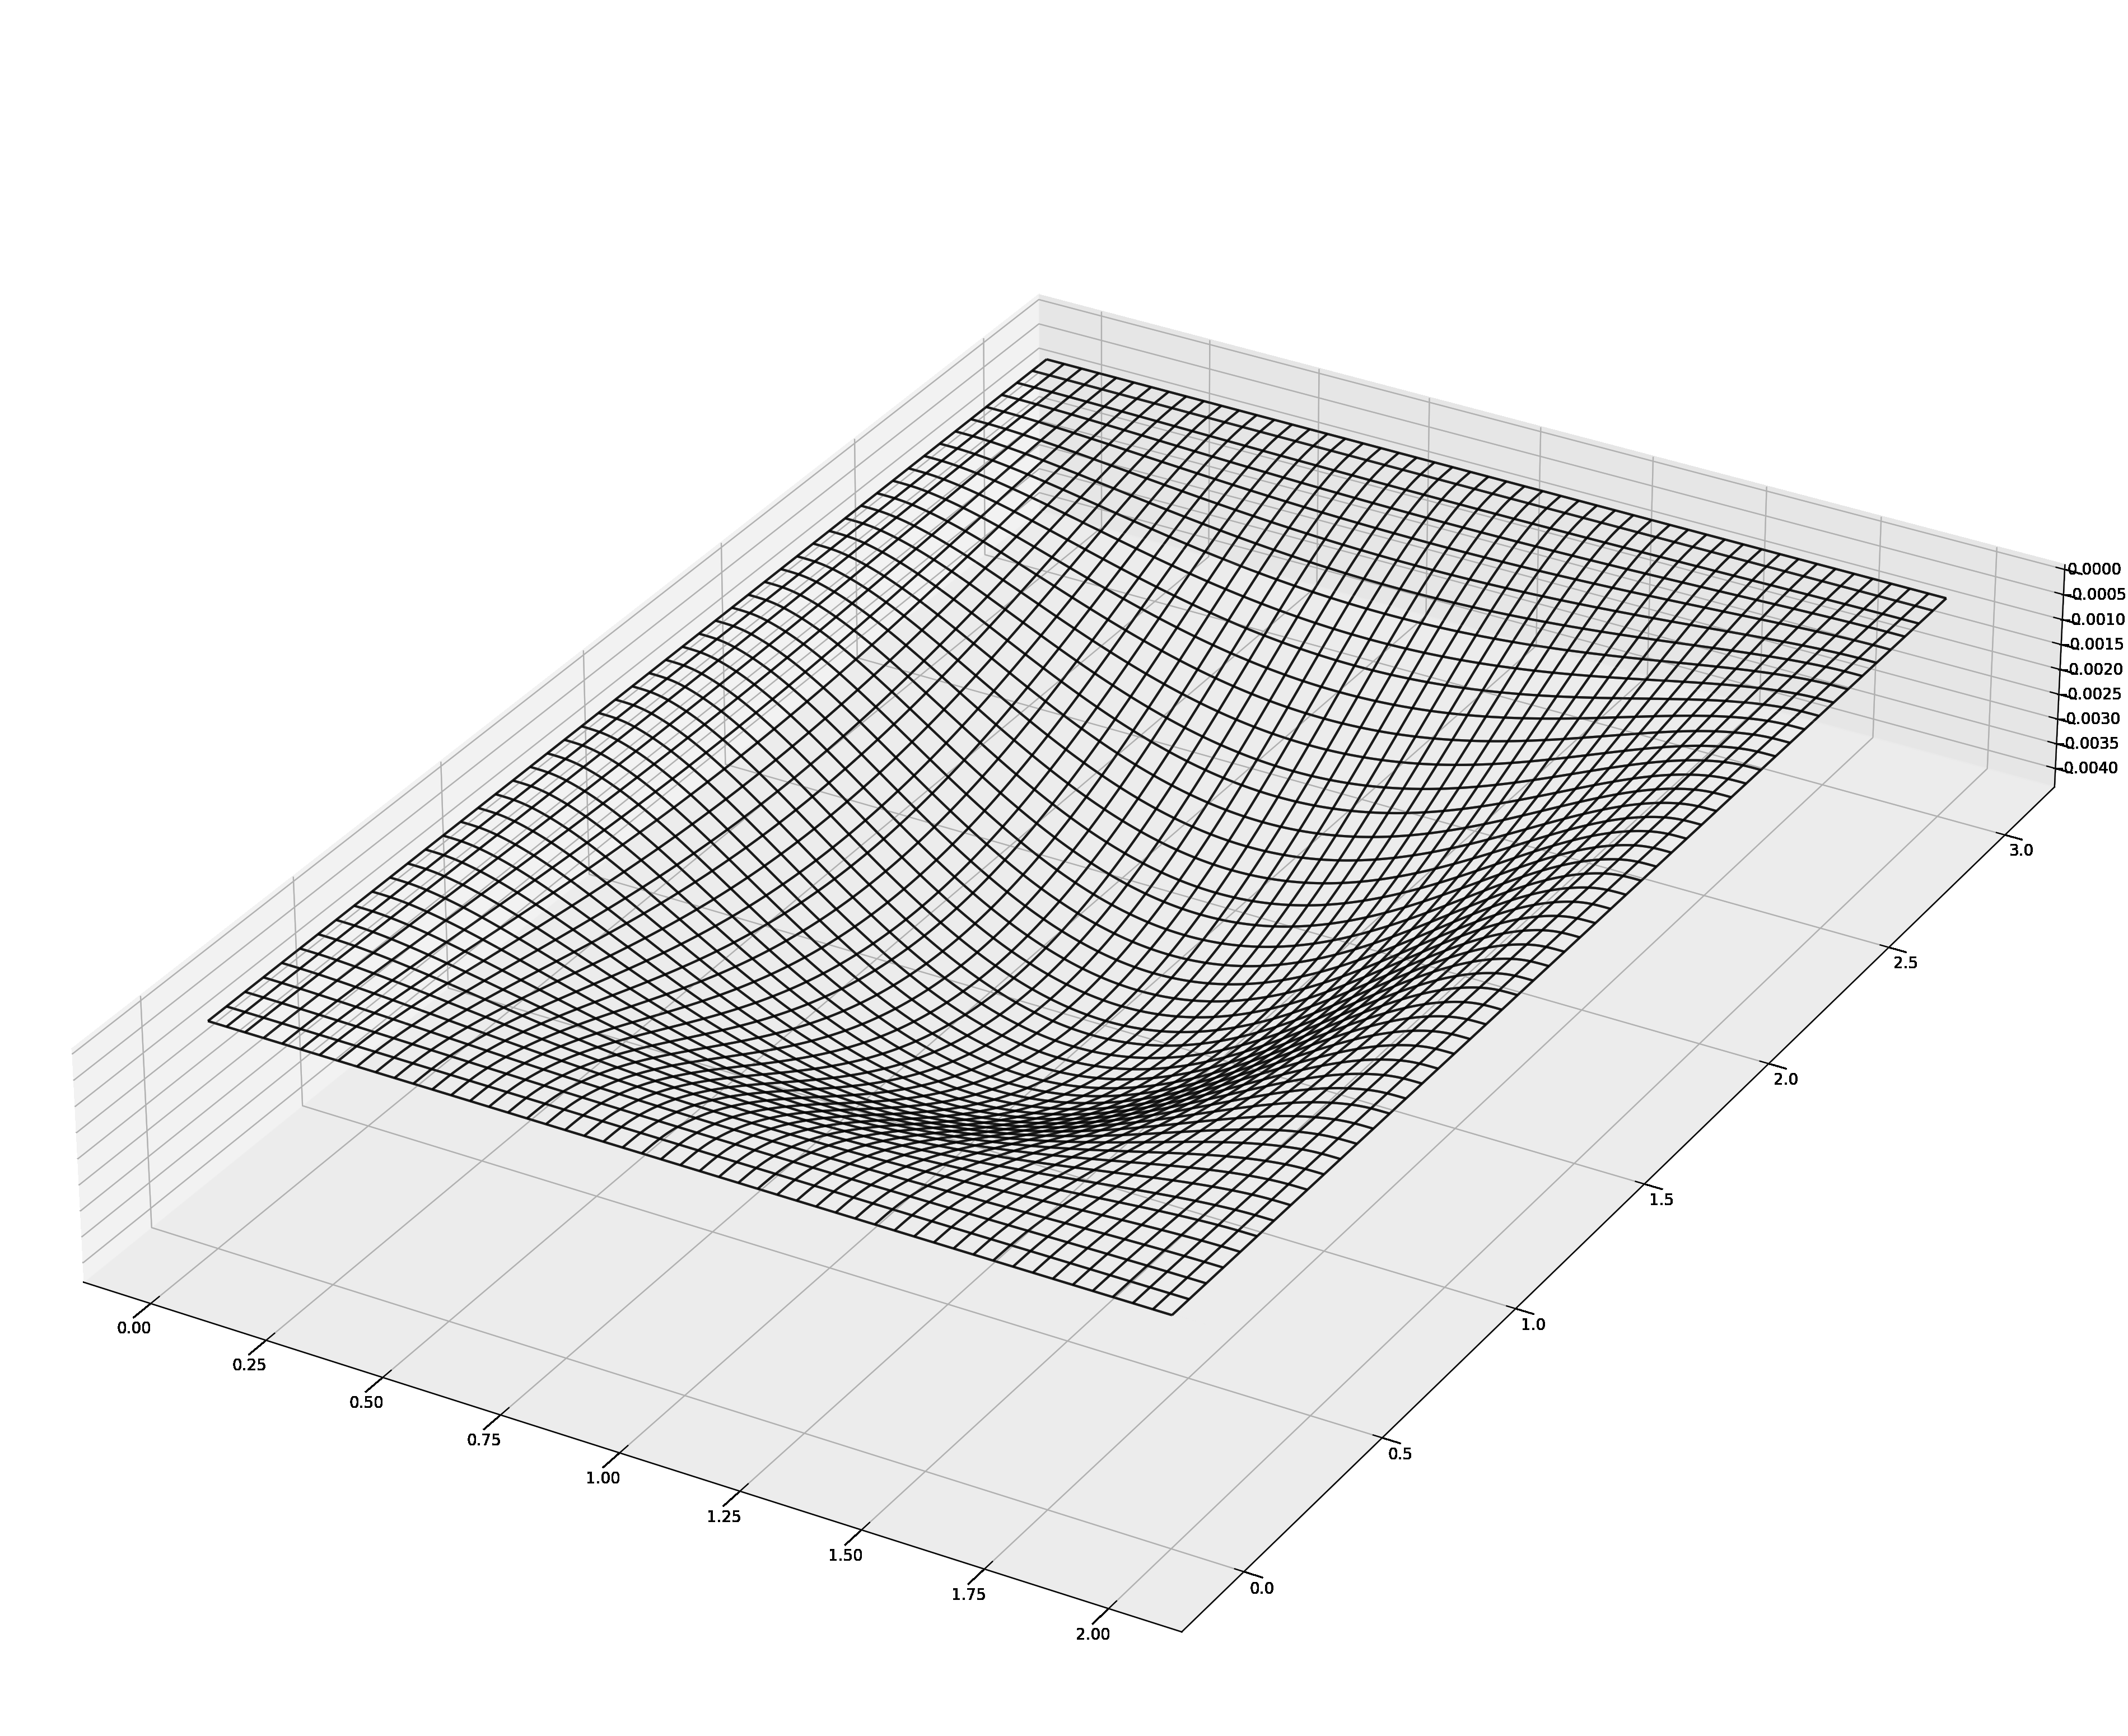
\includegraphics[width=0.9\textwidth]{images/biharmonic_equation_solution}
\captionsetup{labelformat=empty}
\caption{Նկար 4.3. Բիհարմոնիկ հավասարման լուծման գրաֆիկական ներկայացում։}
\end{figure}
\end{document}